% python3 code_to_tex.py nyc25.py nyc25_tex && xelatex </dev/null spork_nyc25.tex
\documentclass[12pt]{article}

\usepackage[a5paper, landscape, margin=10mm]{geometry}
\usepackage{enumitem}
\usepackage{amsmath}
\usepackage{amssymb}
\usepackage{amsfonts}
\usepackage{placeins}
\usepackage{graphicx}
\usepackage{listings}
\usepackage{caption}
\usepackage{colortbl}
\usepackage[parfill]{parskip}
\usepackage[mathscr]{euscript}
\usepackage[usenames,dvipsnames,svgnames,table,hyperref]{xcolor}
\usepackage[hidelinks]{hyperref}
\usepackage{fontspec}
\usepackage{mdframed}

\setsansfont{FreeSans}
\setmonofont{Ubuntu Mono}
\renewcommand{\familydefault}{\sfdefault}

\hyphenation{WebGL}

\definecolor{webColor}{RGB}{0, 108, 174}
\newcommand{\web}[1]{{\color{webColor} \small \url{#1}}}
\newcommand{\webText}[2]{{\color{webColor} \href{#2}{#1}}}
\newcommand{\email}[2]{{\small \color{webColor} \textsf{\href{mailto:#1@#2}{#1[at]#2}}}}
\definecolor{titleColor}{RGB}{179, 0, 149}
\newcommand{\myTitle}[1]{{\large \color{titleColor} \hspace{-4mm} \textbf{\textsf{#1}}}}
\definecolor{subColor}{RGB}{179, 0, 149}
\newcommand{\mySub}[1]{\textsf{\color{subColor}#1}}
\definecolor{keyColor}{RGB}{170, 149, 0}
\newcommand{\myKey}[1]{\textbf{\color{keyColor}#1}}

\definecolor{redBoxFg}{RGB}{255, 0, 0}
\definecolor{redBoxBg}{RGB}{255, 218, 232}
\newcommand{\redBox}[1]{{\color{redBoxFg}\colorbox{redBoxBg}{#1}}}
\definecolor{yellowBoxFg}{RGB}{0, 0, 0}
\definecolor{yellowBoxBg}{RGB}{255, 232, 0}
\newcommand{\yellowBox}[1]{{\color{yellowBoxFg}\colorbox{yellowBoxBg}{#1}}}
\definecolor{greenBoxFg}{RGB}{0, 0, 0}
\definecolor{greenBoxBg}{RGB}{134, 210, 153}
\newcommand{\greenBox}[1]{{\color{greenBoxFg}\colorbox{greenBoxBg}{#1}}}
\definecolor{blueBoxFg}{RGB}{0, 0, 255}
\definecolor{blueBoxBg}{RGB}{218, 232, 255}
\newcommand{\blueBox}[1]{{\color{blueBoxFg}\colorbox{blueBoxBg}{#1}}}
\definecolor{violetBoxFg}{RGB}{0, 0, 0}
\definecolor{violetBoxBg}{RGB}{218, 204, 255}
\newcommand{\violetBox}[1]{{\color{violetBoxFg}\colorbox{violetBoxBg}{#1}}}

\mdfdefinestyle{MyFrame}{%
    linecolor=black,
    outerlinewidth=0pt,
    linewidth=0pt,
    innertopmargin=2.7pt,
    innerbottommargin=0pt,
    innerrightmargin=0pt,
    innerleftmargin=0pt,
        leftmargin = 0pt,
        rightmargin = 0pt}

\definecolor{lightttColor}{RGB}{69, 69, 80}
\newcommand{\lighttt}[1]{{\color{lightttColor}\texttt{#1}}}

\renewcommand*\labelenumi{(\theenumi)}
\renewcommand*{\theenumii}{\roman{enumii}}
\renewcommand*\labelenumii{\theenumii.}

\newcommand{\fixminipage}{\raggedright \setlength{\parskip}{0.3\baselineskip}}
\newcommand{\codeminipage}{\raggedright \setlength{\parskip}{0\baselineskip}}
\sloppy
\pagenumbering{gobble}


\begin{document}

\tikzstyle{smallnode} = [rectangle, minimum width=1.25cm, minimum height=1cm, text centered, text width=1.25cm, draw=black, fill=white]
\tikzstyle{smallishnode} = [rectangle, minimum width=2cm, minimum height=1cm, text centered, text width=2cm, draw=black, fill=white]
\tikzstyle{normalnode} = [rectangle, minimum width=3cm, minimum height=1cm, text centered, text width=3cm, draw=black, fill=white]
\tikzstyle{widenode} = [rectangle, minimum width=62mm, minimum height=8mm, text centered, text width=62mm, draw=black, fill=white]
\tikzstyle{bignode} = [rectangle, minimum width=3.5cm, minimum height=2cm, text centered, text width=3cm, draw=black, fill=white]
\tikzstyle{smemnode} = [rectangle, minimum width=3cm, minimum height=1cm, text centered, text width=3cm, draw=keyColorB, fill=white]
\tikzstyle{gmemnode} = [rectangle, minimum width=3cm, minimum height=1cm, text centered, text width=3cm, draw=keyColorA, fill=white]
\tikzstyle{smallishsmemnode} = [rectangle, minimum width=2cm, minimum height=1cm, text centered, text width=2cm, draw=keyColorB, fill=white]
\tikzstyle{arrow} = [thick,->,>=stealth]
\tikzstyle{line} = [thick]

\tikzstyle{rednode} = [normalnode, draw=redBoxFg, fill=redBoxBg, text=redBoxFg]
\tikzstyle{yellownode} = [normalnode, draw=yellowBoxFg, fill=yellowBoxBg, text=yellowBoxFg]
\tikzstyle{greennode} = [normalnode, draw=greenBoxFg, fill=greenBoxBg, text=greenBoxFg]
\tikzstyle{bluenode} = [normalnode, draw=blueBoxFg, fill=blueBoxBg, text=blueBoxFg]
\tikzstyle{violetnode} = [normalnode, draw=violetBoxFg, fill=violetBoxBg, text=violetBoxFg]

\tikzstyle{redstyle} = [draw=redBoxFg, fill=redBoxBg, text=redBoxFg]
\tikzstyle{yellowstyle} = [draw=yellowBoxFg, fill=yellowBoxBg, text=yellowBoxFg]
\tikzstyle{greenstyle} = [draw=greenBoxFg, fill=greenBoxBg, text=greenBoxFg]
\tikzstyle{bluestyle} = [draw=blueBoxFg, fill=blueBoxBg, text=blueBoxFg]
\tikzstyle{violetstyle} = [draw=violetBoxFg, fill=violetBoxBg, text=violetBoxFg]
\tikzstyle{nRedstyle} = [draw=nRedBoxFg, fill=nRedBoxBg, text=nRedBoxFg]
\tikzstyle{nGoldstyle} = [draw=nGoldBoxFg, fill=nGoldBoxBg, text=nGoldBoxFg]
\tikzstyle{nGreenstyle} = [draw=nGreenBoxFg, fill=nGreenBoxBg, text=nGreenBoxFg]
\tikzstyle{nBluestyle} = [draw=nBlueBoxFg, fill=nBlueBoxBg, text=nBlueBoxFg]
\tikzstyle{nPurplestyle} = [draw=nPurpleBoxFg, fill=nPurpleBoxBg, text=nPurpleBoxFg]

\tikzstyle{Mnode} = [greennode, text width=55mm, minimum width=55mm, minimum height=7mm]
\tikzstyle{Nnode} = [violetnode, text width=7mm, minimum width=7mm, minimum height=7mm]

\tikzstyle{producer} = [yellownode, text width=64mm, minimum width=64mm, minimum height=14mm]
\tikzstyle{consumer} = [greennode, text width=20mm, minimum width=20mm, minimum height=14mm]
\tikzstyle{smallproducer} = [yellownode, text width=20mm, minimum width=20mm, minimum height=14mm]
\tikzstyle{copylatency} = [violetnode, text width=84mm, minimum width=84mm, minimum height=8mm]
\tikzstyle{ring} = [violetnode, text width=16mm, minimum width=1mm, minimum height=14mm]
\newcommand{\consumerBox}[1]{{\color{greenBoxFg}\colorbox{greenBoxBg}{#1}}}
\newcommand{\producerBox}[1]{{\color{yellowBoxFg}\colorbox{yellowBoxBg}{#1}}}

\myBiggerTitle{Exo-GPU}

\textbf{\hfill \Large Safe, Imperative, User-schedulable Programming for Tensor Cores}

{\LARGE

\vfill

David Zhao Akeley

Yuka Ikarashi

Jonathan Ragan-Kelley

\hfill \myBiggerTitle{2025 MIT/Jane Street Symposium}}

%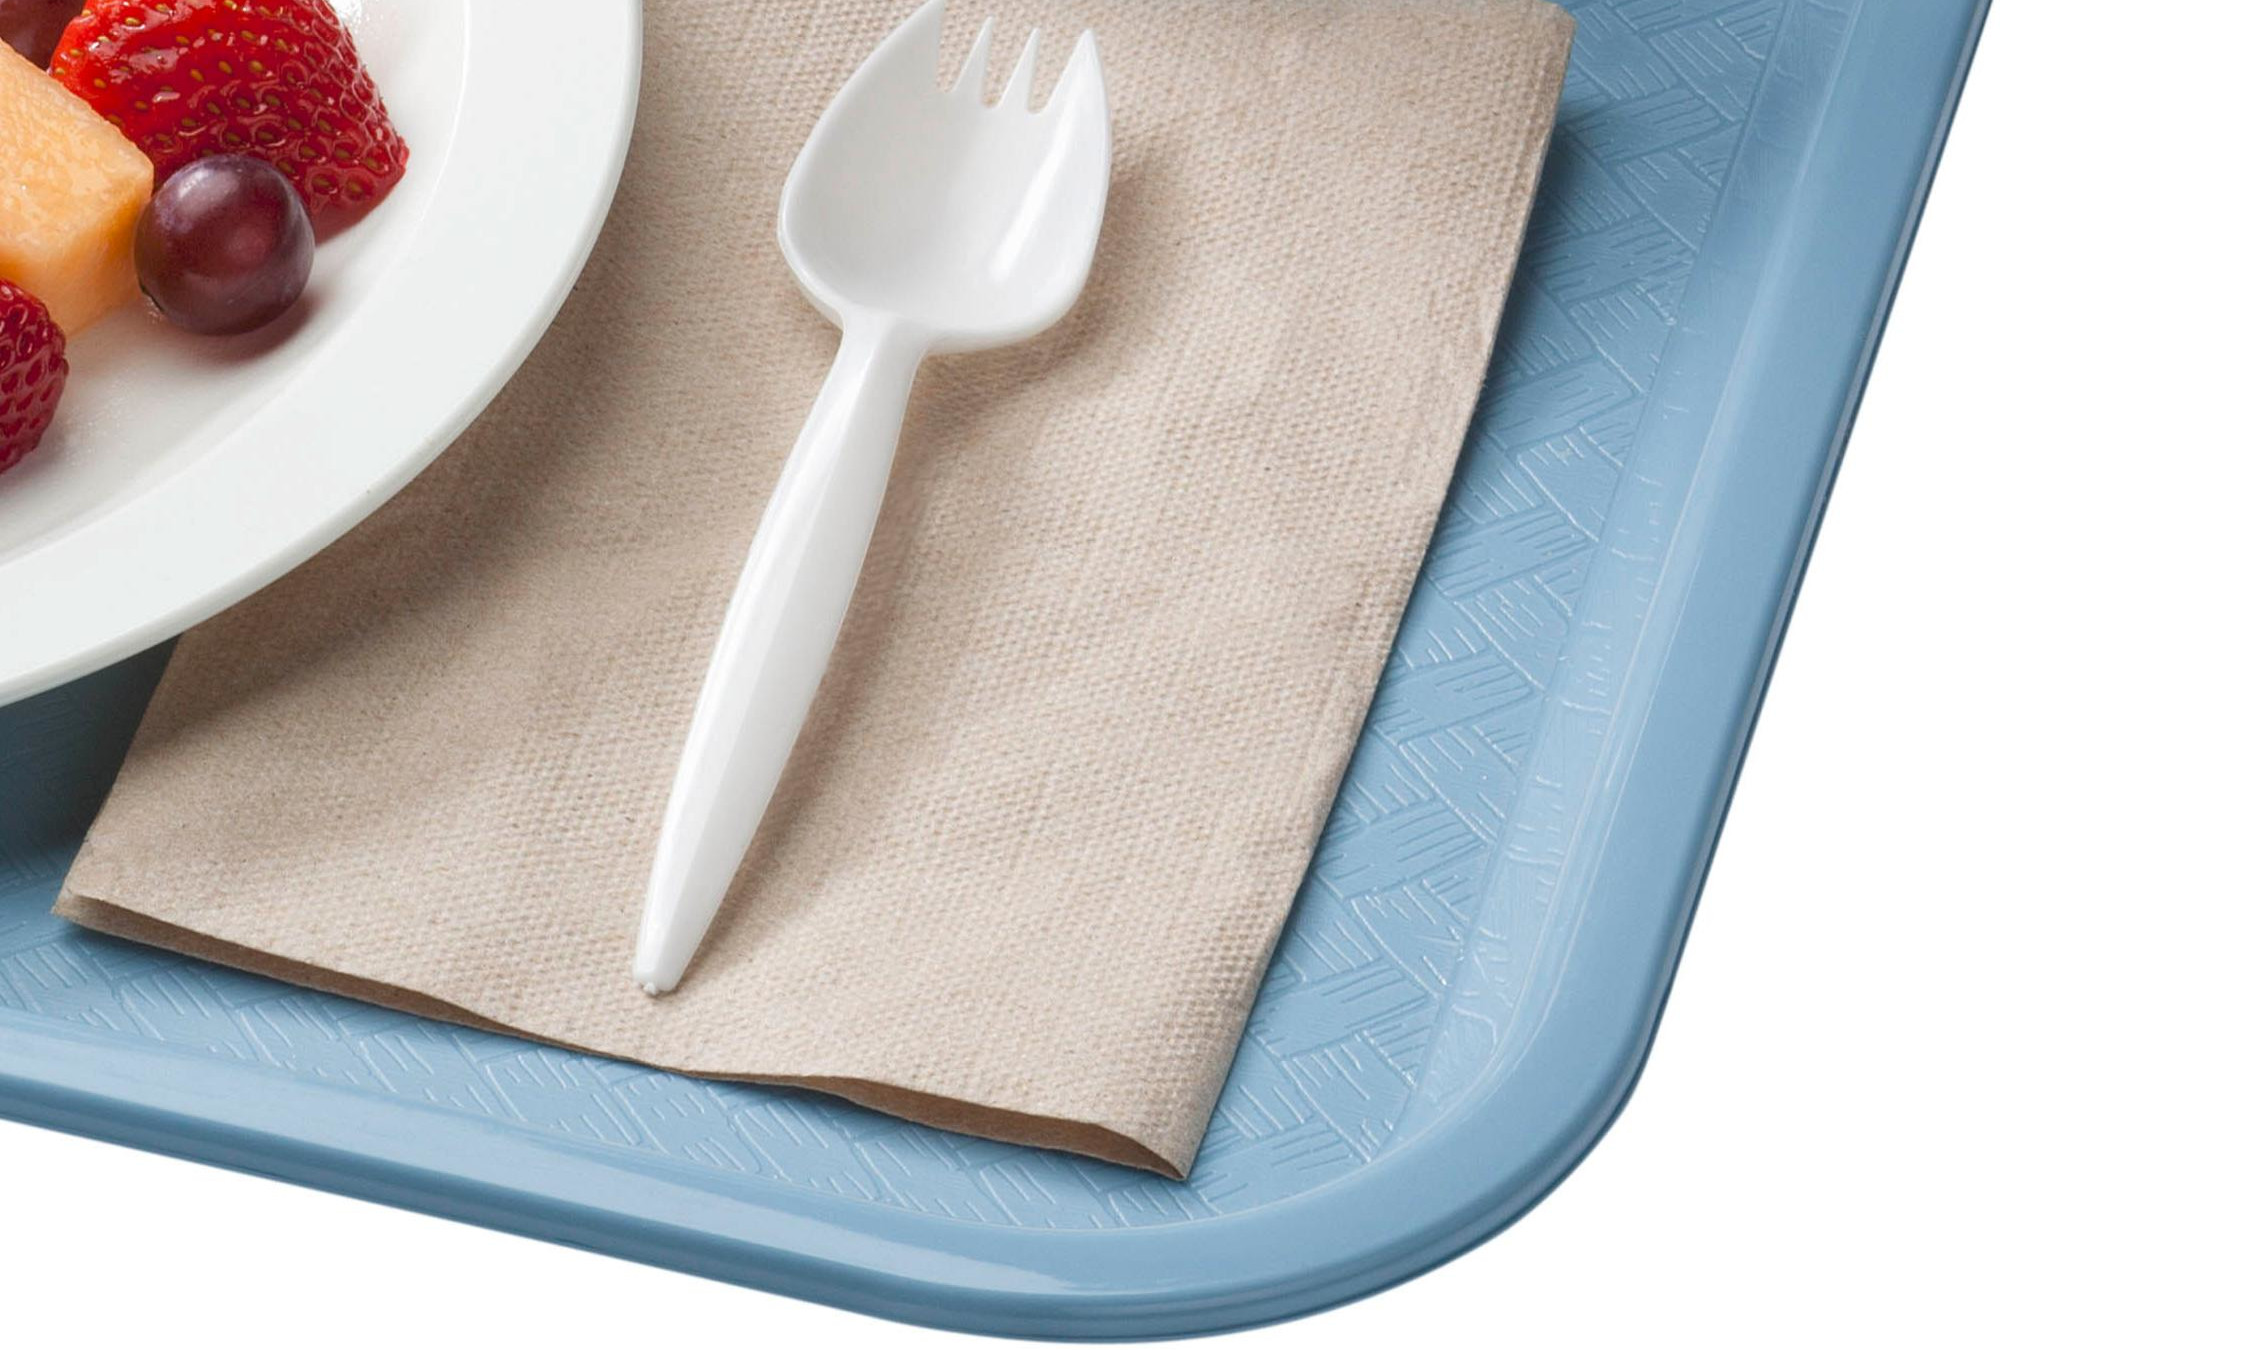
\includegraphics[width=\linewidth]{usda_spork.jpg}

\newpage
\myBiggerTitle{Starting out with Exo \hfill \nBlueBox{GEMM v1}}

{\large
\input{nyc25_tex/cpu.0.tex}
}

\vspace{3mm}
\hrule

{\LARGE
\texttt{@proc} (procedure) decorator
\begin{itemize}
  \item Python AST $\to$ C/C++ (mostly 1:1)
\end{itemize}

}

\newpage
\myBiggerTitle{Starting out with Exo \hfill \nBlueBox{GEMM v1}}

{\large
\input{nyc25_tex/cpu.3.tex}
}

\vspace{3mm}
\hrule

{\LARGE
\texttt{seq}-loop $\mapsto$ \texttt{for (\textit{int var} = lo; \textit{var} < hi; ++\textit{var})}

\myKeyA{Sequential} loops here; contrast to \myKeyB{parallel} loops later.

}

\newpage
\myBiggerTitle{Type Annotations \hfill \nBlueBox{GEMM v1}}

{\large
\input{nyc25_tex/cpu.1.tex}
}

\newpage
\myBiggerTitle{Memory Type Annotations \hfill \nBlueBox{GEMM v1}}

{\large
\input{nyc25_tex/cpu.2.tex}
}

\newpage
\myBiggerTitle{Exo Rewrites}

\begin{center}
{\large
\begin{tikzpicture}[node distance=8mm]
\node(proc0) [normalnode, text width=2cm, minimum width=2cm] {Original proc $p_0$};
\node(proc1) [normalnode, text width=2cm, minimum width=2cm, right=of proc0] {$p_1, p_2,...$};
\node(procNS) [normalnode, right=of proc1, text width=4cm, minimum width=4cm] {Final proc $p_n$};
\node(c) [normalnode, right=of procNS] {C code};

\draw [arrow] (proc0) -- (proc1);
\draw [arrow] (proc1.north east) to[out=45, in=90] (proc1.north);
\draw [arrow] (proc1) to node(p1arrow)[]{} (procNS);
\draw [arrow] (procNS) to node(toC)[]{} (c);

\node(exo) [normalnode, yshift=-4mm, text width=4cm, minimum width=4cm, below=of p1arrow, draw=blueBoxFg, fill=blueBoxBg, text=blueBoxFg] {Exo Rewrites};
\node(codegen) [normalnode, yshift=-4mm, text width=6cm, xshift=1cm, below=of toC, draw=blueBoxFg, fill=blueBoxBg, text=blueBoxFg] {Code Generator};
\node(equiv) [left=of exo, text=blueBoxFg, xshift=9mm] {\textbf{Equivalence due to:}};

\draw [line, draw=blueBoxFg] (exo.north) to[out=135, in=270] (proc0.south west);
\draw [line, draw=blueBoxFg] (exo.north) to[out=45, in=270] (procNS.south);
\draw [line, draw=blueBoxFg] (codegen.north) to[out=135, in=270] (procNS.south);
\draw [line, draw=blueBoxFg] (codegen.north) to[out=45, in=270] (c.south east);
\draw [arrow] (procNS.east) to (c.west);

\end{tikzpicture}
}
\end{center}

{\LARGE
Process of optimization:
\begin{itemize}
  \item \texttt{proc} internals change.
  \item \myKeyA{Functional equivalence} preserved:\\ Same outputs for same inputs (``same behavior'').
\end{itemize}

}
\vfill
\hrule
{\large
\textit{Exocompilation for Productive Programming of Hardware Accelerators}\\
Y. Ikarashi, G. Bernstein, A. Reinking, H. Genc, J. Ragan-Kelley.
PLDI 2022\\
\textit{Exo 2: Growing a Scheduling Language}\\
Y. Ikarashi, K. Qian, S. Droubi, A. Reinking, G. Bernstein, J. Ragan-Kelley.
ASPLOS 2025 

}


\newpage
\myBiggerTitle{Exo Rewrites}

\begin{center}
{\large
\begin{tikzpicture}[node distance=8mm]
\node(proc0) [normalnode, text width=2cm, minimum width=2cm] {Original proc $p_0$};
\node(proc1) [normalnode, text width=2cm, minimum width=2cm, right=of proc0] {$p_1, p_2,...$};
\node(procNS) [normalnode, right=of proc1, text width=4cm, minimum width=4cm] {Final proc $p_n$};
\node(c) [normalnode, right=of procNS] {C code};

\draw [arrow] (proc0) -- (proc1);
\draw [arrow] (proc1.north east) to[out=45, in=90] (proc1.north);
\draw [arrow] (proc1) to node(p1arrow)[]{} (procNS);
\draw [arrow] (procNS) to node(toC)[]{} (c);

\node(exo) [normalnode, yshift=-4mm, text width=4cm, minimum width=4cm, below=of p1arrow, draw=blueBoxFg, fill=blueBoxBg, text=blueBoxFg] {Exo Rewrites};
\node(codegen) [normalnode, yshift=-4mm, text width=6cm, xshift=1cm, below=of toC, draw=blueBoxFg, fill=blueBoxBg, text=blueBoxFg] {Code Generator};
\node(equiv) [left=of exo, text=blueBoxFg, xshift=9mm] {\textbf{Equivalence due to:}};

\draw [line, draw=blueBoxFg] (exo.north) to[out=135, in=270] (proc0.south west);
\draw [line, draw=blueBoxFg] (exo.north) to[out=45, in=270] (procNS.south);
\draw [line, draw=blueBoxFg] (codegen.north) to[out=135, in=270] (procNS.south);
\draw [line, draw=blueBoxFg] (codegen.north) to[out=45, in=270] (c.south east);
\draw [arrow] (procNS.east) to (c.west);

\end{tikzpicture}
}
\end{center}

{\LARGE
\myKeyA{User-schedulable} paradigm:
\begin{itemize}
  \item Start with a simple \texttt{proc}.
  \item Issue a series of \myKeyA{behavior-preserving rewrite rules}.
  \begin{itemize}
    \item (metaprogram with Python)
  \end{itemize}
  \item $p_n$ proven functionally equivalent to $p_0$; may be faster.
\end{itemize}

}
\vfill
\hrule
{\large
\textit{Exocompilation for Productive Programming of Hardware Accelerators}\\
Y. Ikarashi, G. Bernstein, A. Reinking, H. Genc, J. Ragan-Kelley.
PLDI 2022\\
\textit{Exo 2: Growing a Scheduling Language}\\
Y. Ikarashi, K. Qian, S. Droubi, A. Reinking, G. Bernstein, J. Ragan-Kelley.
ASPLOS 2025 

}


\newpage
\myBiggerTitle{Exo Rewrites}

\begin{center}
{\large
\begin{tikzpicture}[node distance=8mm]
\node(proc0) [normalnode, text width=2cm, minimum width=2cm] {Original proc $p_0$};
\node(proc1) [normalnode, text width=2cm, minimum width=2cm, right=of proc0] {$p_1, p_2,...$};
\node(procNS) [normalnode, right=of proc1, text width=4cm, minimum width=4cm] {Final proc $p_n$};
\node(c) [normalnode, right=of procNS] {C code};

\draw [arrow] (proc0) -- (proc1);
\draw [arrow] (proc1.north east) to[out=45, in=90] (proc1.north);
\draw [arrow] (proc1) to node(p1arrow)[]{} (procNS);
\draw [arrow] (procNS) to node(toC)[]{} (c);

\node(exo) [normalnode, yshift=-4mm, text width=4cm, minimum width=4cm, below=of p1arrow, draw=blueBoxFg, fill=blueBoxBg, text=blueBoxFg] {Exo Rewrites};
\node(codegen) [normalnode, yshift=-4mm, text width=6cm, xshift=1cm, below=of toC, draw=blueBoxFg, fill=blueBoxBg, text=blueBoxFg] {Code Generator};
\node(equiv) [left=of exo, text=blueBoxFg, xshift=9mm] {\textbf{Equivalence due to:}};

\draw [line, draw=blueBoxFg] (exo.north) to[out=135, in=270] (proc0.south west);
\draw [line, draw=blueBoxFg] (exo.north) to[out=45, in=270] (procNS.south);
\draw [line, draw=blueBoxFg] (codegen.north) to[out=135, in=270] (procNS.south);
\draw [line, draw=blueBoxFg] (codegen.north) to[out=45, in=270] (c.south east);
\draw [arrow] (procNS.east) to (c.west);

\end{tikzpicture}
}
\end{center}

{\LARGE
\begin{itemize}
  \item Can optimize for \myKeyA{efficient memory access}.
  \item Can target specialized CPU instructions today:\\e.g. GEMMINI, Intel AMX, ARM SME
\end{itemize}
Goal: extend rewrite model \& underlying semantics to model\\\myKeyB{imperative GPU programming} in a disciplined way.

}
\vfill
\hrule
{\large
\textit{Exocompilation for Productive Programming of Hardware Accelerators}\\
Y. Ikarashi, G. Bernstein, A. Reinking, H. Genc, J. Ragan-Kelley.
PLDI 2022\\
\textit{Exo 2: Growing a Scheduling Language}\\
Y. Ikarashi, K. Qian, S. Droubi, A. Reinking, G. Bernstein, J. Ragan-Kelley.
ASPLOS 2025 

}


\newpage
\myBiggerTitle{M/N Tiling \hfill \nBlueBox{GEMM v1}}

{\large
\input{nyc25_tex/cpu.3.tex}
}

\vspace{3mm}
\hrule

{\LARGE
We want to \myKeyA{tile} the \greenBox{m}/\violetBox{n} loop nest.

}


\newpage
\myBiggerTitle{Divide Loop (M)}

{\large
\input{nyc25_tex/m_divide_loop.0.tex}
}

\newpage
\myBiggerTitle{M Variable Rewritten}

{\large
\input{nyc25_tex/m_divide_loop.1.tex}
}

\newpage
\myBiggerTitle{Assume Perfect Tiling}

{\large
\input{nyc25_tex/m_divide_loop.2.tex}
}

\newpage
\myBiggerTitle{Divide Loop (N)}

{\large
\input{nyc25_tex/n_divide_loop.0.tex}
}

\newpage
\myBiggerTitle{Reorder Loops}

{\large
\input{nyc25_tex/reorder_loops.0.tex}
}

\newpage
{\large
\textbf{\LARGE BEFORE}\\
\input{nyc25_tex/cpu.4.tex}
}

\vspace{1mm}
\hrule

{\large
{\LARGE \textbf{AFTER} (Exo checked functional equivalence)}\\
\input{nyc25_tex/reorder_loops.1.tex}
}

\newpage
\myBiggerTitle{GPU: Blocks \& Threads}

{\LARGE

Goal: Map tiles to different levels of the GPU hierarchy

\begin{itemize}
\item Launch \myKeyA{grid} of CUDA threads from \myKeyA{CPU}.
\item Map work to CUDA threads with \myKeyB{parallel for} loops.
\end{itemize}

}

\vfill
\begin{tikzpicture}[node distance=2mm]
\node (grid) [normalnode, nRedstyle, text width=5cm, minimum width=5cm] {\textbf{grid}};
\node (cpu) [left=of grid, xshift=-2cm] {\textbf{CPU}};
\node (cpuDummy) [anchor=east] at(cpu.west) {\ };  % Aligns diagram slightly to the right.
\draw [arrow] (cpu) -- node[above] {\textbf{launch}} (grid);
\node (cuda) [above=of grid, yshift=+4mm] {\textbf{CUDA Constructs}};
\node (exo) [right=of cuda, xshift=25mm] {\textbf{Exo-GPU Constructs}};

\node (cta0) [normalnode, nGoldstyle, text width=20mm, minimum width=20mm, below=of grid, xshift=-15mm, yshift=-1cm] {\textbf{block}};
\node (cta1) [normalnode, nGoldstyle, text width=20mm, minimum width=20mm, below=of grid, xshift=+15mm, yshift=-1cm] {\textbf{block}};

\node (thread0) [normalnode, nGreenstyle, text width=16mm, minimum width=16mm, below=of cta0, yshift=-1cm, xshift=-32mm] {\textbf{thread}};
\node (thread1) [normalnode, nGreenstyle, text width=16mm, minimum width=16mm, right=of thread0] {\textbf{thread}};
\node (thread2) [normalnode, nGreenstyle, text width=16mm, minimum width=16mm, right=of thread1, xshift=22mm] {\textbf{thread}};

\draw [arrow] (grid.south) to[out=270, in=90] (cta0.north);
\draw [arrow] (grid.south) to[out=270, in=90] (cta1.north);

\draw [arrow] (cta0.south) to[out=250, in=90] (thread0.north);
\draw [arrow] (cta0.south) to[out=270, in=90] (thread1.north);
\draw [arrow] (cta0.south) to[out=270, in=90] (thread2.north);
\draw [dotted] (thread1.east) -- (thread2.west);

\node (blockDim) [yshift=-1cm] at ($(thread0.south)!0.5!(thread2.south)$) {\blueBox{blockDim}};
\draw [thick, bluestyle, fill=none] ($(thread0.south west) + (0.01, 0)$) to[out=270, in=90] (blockDim.north);
\draw [thick, bluestyle, fill=none] ($(thread2.south east) - (0.01, 0)$) to[out=270, in=90] (blockDim.north);
% Slight offset by 0.01 needed otherwise there is a mystery page break

\node (CudaDeviceFunction) [align=left, right=of grid, text width=100mm] {\large\texttt{\codecomment{\# CPU launches grid}\\with \nRedBox{\textbf{CudaDeviceFunction}}(\blueBox{blockDim=\textit{arg}}):\\~~\codecomment{\# Body lowered to CUDA C++}}\\};
\node (cudaTasks) [align=left, right=of cta1, text width=100mm] {\large\texttt{~~for \textit{iter} in \nGoldBox{\textbf{cuda\_tasks}}(\textit{lo}, \textit{hi}):}\\};
\node (cudaThreads) [align=left, right=of thread2, text width=110mm] {\large\texttt{~~~~for \textit{iter} in \nGreenBox{\textbf{cuda\_threads}}(\textit{lo}, \textit{hi}, unit=\textit{u}):}\\};

\end{tikzpicture}


\newpage
\myBiggerTitle{GPU: Blocks \& Threads}

{\LARGE

Goal: Map tiles to different levels of the GPU hierarchy

\begin{itemize}
\item Launch \myKeyA{grid} of CUDA threads from \myKeyA{CPU}.
\item Map work to CUDA threads with \myKeyB{parallel for} loops.
\end{itemize}

}

\vfill
\begin{tikzpicture}[node distance=2mm]
\node (grid) [normalnode, nRedstyle, text width=5cm, minimum width=5cm] {\textbf{grid}};
\node (cpu) [left=of grid, xshift=-2cm] {\textbf{CPU}};
\node (cpuDummy) [anchor=east] at(cpu.west) {\ };  % Aligns diagram slightly to the right.
\draw [arrow] (cpu) -- node[above] {\textbf{launch}} (grid);
\node (cuda) [above=of grid, yshift=+4mm] {\textbf{CUDA Constructs}};
\node (exo) [right=of cuda, xshift=25mm] {\textbf{Exo-GPU Constructs}};

\node (cta0) [normalnode, nGoldstyle, text width=20mm, minimum width=20mm, below=of grid, xshift=-15mm, yshift=-1cm] {\textbf{block}};
\node (cta1) [normalnode, nGoldstyle, text width=20mm, minimum width=20mm, below=of grid, xshift=+15mm, yshift=-1cm] {\textbf{block}};

\node (thread0) [normalnode, nGreenstyle, text width=16mm, minimum width=16mm, below=of cta0, yshift=-1cm, xshift=-32mm] {\textbf{thread}};
\node (thread1) [normalnode, nGreenstyle, text width=16mm, minimum width=16mm, right=of thread0] {\textbf{thread}};
\node (thread2) [normalnode, nGreenstyle, text width=16mm, minimum width=16mm, right=of thread1, xshift=22mm] {\textbf{thread}};

\draw [arrow] (grid.south) to[out=270, in=90] (cta0.north);
\draw [arrow] (grid.south) to[out=270, in=90] (cta1.north);

\draw [arrow] (cta0.south) to[out=250, in=90] (thread0.north);
\draw [arrow] (cta0.south) to[out=270, in=90] (thread1.north);
\draw [arrow] (cta0.south) to[out=270, in=90] (thread2.north);
\draw [dotted] (thread1.east) -- (thread2.west);

\node (blockDim) [yshift=-1cm] at ($(thread0.south)!0.5!(thread2.south)$) {\blueBox{blockDim}};
\draw [thick, bluestyle, fill=none] ($(thread0.south west) + (0.01, 0)$) to[out=270, in=90] (blockDim.north);
\draw [thick, bluestyle, fill=none] ($(thread2.south east) - (0.01, 0)$) to[out=270, in=90] (blockDim.north);
% Slight offset by 0.01 needed otherwise there is a mystery page break

\node (CudaDeviceFunction) [align=left, right=of grid, text width=100mm] {\large\texttt{\codecomment{\# CPU launches grid}\\with \nRedBox{\textbf{CudaDeviceFunction}}(\blueBox{blockDim=\textit{arg}}):\\~~\codecomment{\# Body lowered to CUDA C++}}\\};
\node (cudaTasks) [align=left, right=of cta1, text width=100mm] {\large\texttt{~~for \textit{iter} in \nGoldBox{\textbf{cuda\_tasks}}(\textit{lo}, \textit{hi}):}\\};
\node (cudaThreads) [align=left, right=of thread2, text width=110mm] {\large\texttt{~~~~for \textit{iter} in \nGreenBox{\textbf{cuda\_threads}}(\textit{lo}, \textit{hi}, unit=\textit{u}):}\\};

\draw [ultra thick, draw=magenta] ($(grid.north west) + (-3.38, 0.25)$) -- ($(grid.north east) + (0.25, 0.25)$);
\draw [ultra thick, draw=magenta] ($(grid.south west) + (-3.38, -0.25)$) -- ($(grid.south east) + (0.25, -0.25)$);
\draw [ultra thick, draw=magenta] ($(grid.north west) + (-3.38, 0.25)$) -- ($(grid.south west) + (-3.38, -0.25)$);
\draw [ultra thick, draw=magenta] ($(grid.south east) + (0.25, -0.25)$) -- ($(grid.north east) + (0.25, 0.25)$);
\end{tikzpicture}


\newpage
\myBiggerTitle{GPU: Blocks \& Threads}

{\LARGE

Goal: Map tiles to different levels of the GPU hierarchy

\begin{itemize}
\item Launch \myKeyA{grid} of CUDA threads from \myKeyA{CPU}.
\item Map work to CUDA threads with \myKeyB{parallel for} loops.
\end{itemize}

}

\vfill
\begin{tikzpicture}[node distance=2mm]
\node (grid) [normalnode, nRedstyle, text width=5cm, minimum width=5cm] {\textbf{grid}};
\node (cpu) [left=of grid, xshift=-2cm] {\textbf{CPU}};
\node (cpuDummy) [anchor=east] at(cpu.west) {\ };  % Aligns diagram slightly to the right.
\draw [arrow] (cpu) -- node[above] {\textbf{launch}} (grid);
\node (cuda) [above=of grid, yshift=+4mm] {\textbf{CUDA Constructs}};
\node (exo) [right=of cuda, xshift=25mm] {\textbf{Exo-GPU Constructs}};

\node (cta0) [normalnode, nGoldstyle, text width=20mm, minimum width=20mm, below=of grid, xshift=-15mm, yshift=-1cm] {\textbf{block}};
\node (cta1) [normalnode, nGoldstyle, text width=20mm, minimum width=20mm, below=of grid, xshift=+15mm, yshift=-1cm] {\textbf{block}};

\node (thread0) [normalnode, nGreenstyle, text width=16mm, minimum width=16mm, below=of cta0, yshift=-1cm, xshift=-32mm] {\textbf{thread}};
\node (thread1) [normalnode, nGreenstyle, text width=16mm, minimum width=16mm, right=of thread0] {\textbf{thread}};
\node (thread2) [normalnode, nGreenstyle, text width=16mm, minimum width=16mm, right=of thread1, xshift=22mm] {\textbf{thread}};

\draw [arrow] (grid.south) to[out=270, in=90] (cta0.north);
\draw [arrow] (grid.south) to[out=270, in=90] (cta1.north);

\draw [arrow] (cta0.south) to[out=250, in=90] (thread0.north);
\draw [arrow] (cta0.south) to[out=270, in=90] (thread1.north);
\draw [arrow] (cta0.south) to[out=270, in=90] (thread2.north);
\draw [dotted] (thread1.east) -- (thread2.west);

\node (blockDim) [yshift=-1cm] at ($(thread0.south)!0.5!(thread2.south)$) {\blueBox{blockDim}};
\draw [thick, bluestyle, fill=none] ($(thread0.south west) + (0.01, 0)$) to[out=270, in=90] (blockDim.north);
\draw [thick, bluestyle, fill=none] ($(thread2.south east) - (0.01, 0)$) to[out=270, in=90] (blockDim.north);
% Slight offset by 0.01 needed otherwise there is a mystery page break

\node (CudaDeviceFunction) [align=left, right=of grid, text width=100mm] {\large\texttt{\codecomment{\# CPU launches grid}\\with \nRedBox{\textbf{CudaDeviceFunction}}(\blueBox{blockDim=\textit{arg}}):\\~~\codecomment{\# Body lowered to CUDA C++}}\\};
\node (cudaTasks) [align=left, right=of cta1, text width=100mm] {\large\texttt{~~for \textit{iter} in \nGoldBox{\textbf{cuda\_tasks}}(\textit{lo}, \textit{hi}):}\\};
\node (cudaThreads) [align=left, right=of thread2, text width=110mm] {\large\texttt{~~~~for \textit{iter} in \nGreenBox{\textbf{cuda\_threads}}(\textit{lo}, \textit{hi}, unit=\textit{u}):}\\};

\draw [ultra thick, draw=magenta] ($(cta0.north west) + (-3.38, 0.25)$) -- ($(cta1.north east) + (0.25, 0.25)$);
\draw [ultra thick, draw=magenta] ($(cta0.south west) + (-3.38, -0.25)$) -- ($(cta1.south east) + (0.25, -0.25)$);
\draw [ultra thick, draw=magenta] ($(cta0.north west) + (-3.38, 0.25)$) -- ($(cta0.south west) + (-3.38, -0.25)$);
\draw [ultra thick, draw=magenta] ($(cta1.south east) + (0.25, -0.25)$) -- ($(cta1.north east) + (0.25, 0.25)$);
\draw [ultra thick, draw=magenta] ($(CudaDeviceFunction.north west) + (+4.75, 0.05)$) -- ($(CudaDeviceFunction.north east) + (0.05, 0.05)$);
\draw [ultra thick, draw=magenta] ($(CudaDeviceFunction.south west) + (+4.75, -0.05)$) -- ($(CudaDeviceFunction.south east) + (0.05, -0.05)$);
\draw [ultra thick, draw=magenta] ($(CudaDeviceFunction.north west) + (+4.75, 0.05)$) -- ($(CudaDeviceFunction.south west) + (+4.75, -0.05)$);
\draw [ultra thick, draw=magenta] ($(CudaDeviceFunction.south east) + (0.05, -0.05)$) -- ($(CudaDeviceFunction.north east) + (0.05, 0.05)$);
\end{tikzpicture}


\newpage
\myBiggerTitle{GPU: Blocks \& Threads}

{\LARGE

Goal: Map tiles to different levels of the GPU hierarchy

\begin{itemize}
\item Launch \myKeyA{grid} of CUDA threads from \myKeyA{CPU}.
\item Map work to CUDA threads with \myKeyB{parallel for} loops.
\end{itemize}

}

\vfill
\begin{tikzpicture}[node distance=2mm]
\node (grid) [normalnode, nRedstyle, text width=5cm, minimum width=5cm] {\textbf{grid}};
\node (cpu) [left=of grid, xshift=-2cm] {\textbf{CPU}};
\node (cpuDummy) [anchor=east] at(cpu.west) {\ };  % Aligns diagram slightly to the right.
\draw [arrow] (cpu) -- node[above] {\textbf{launch}} (grid);
\node (cuda) [above=of grid, yshift=+4mm] {\textbf{CUDA Constructs}};
\node (exo) [right=of cuda, xshift=25mm] {\textbf{Exo-GPU Constructs}};

\node (cta0) [normalnode, nGoldstyle, text width=20mm, minimum width=20mm, below=of grid, xshift=-15mm, yshift=-1cm] {\textbf{block}};
\node (cta1) [normalnode, nGoldstyle, text width=20mm, minimum width=20mm, below=of grid, xshift=+15mm, yshift=-1cm] {\textbf{block}};

\node (thread0) [normalnode, nGreenstyle, text width=16mm, minimum width=16mm, below=of cta0, yshift=-1cm, xshift=-32mm] {\textbf{thread}};
\node (thread1) [normalnode, nGreenstyle, text width=16mm, minimum width=16mm, right=of thread0] {\textbf{thread}};
\node (thread2) [normalnode, nGreenstyle, text width=16mm, minimum width=16mm, right=of thread1, xshift=22mm] {\textbf{thread}};

\draw [arrow] (grid.south) to[out=270, in=90] (cta0.north);
\draw [arrow] (grid.south) to[out=270, in=90] (cta1.north);

\draw [arrow] (cta0.south) to[out=250, in=90] (thread0.north);
\draw [arrow] (cta0.south) to[out=270, in=90] (thread1.north);
\draw [arrow] (cta0.south) to[out=270, in=90] (thread2.north);
\draw [dotted] (thread1.east) -- (thread2.west);

\node (blockDim) [yshift=-1cm] at ($(thread0.south)!0.5!(thread2.south)$) {\blueBox{blockDim}};
\draw [thick, bluestyle, fill=none] ($(thread0.south west) + (0.01, 0)$) to[out=270, in=90] (blockDim.north);
\draw [thick, bluestyle, fill=none] ($(thread2.south east) - (0.01, 0)$) to[out=270, in=90] (blockDim.north);
% Slight offset by 0.01 needed otherwise there is a mystery page break

\node (CudaDeviceFunction) [align=left, right=of grid, text width=100mm] {\large\texttt{\codecomment{\# CPU launches grid}\\with \nRedBox{\textbf{CudaDeviceFunction}}(\blueBox{blockDim=\textit{arg}}):\\~~\codecomment{\# Body lowered to CUDA C++}}\\};
\node (cudaTasks) [align=left, right=of cta1, text width=100mm] {\large\texttt{~~for \textit{iter} in \nGoldBox{\textbf{cuda\_tasks}}(\textit{lo}, \textit{hi}):}\\};
\node (cudaThreads) [align=left, right=of thread2, text width=110mm] {\large\texttt{~~~~for \textit{iter} in \nGreenBox{\textbf{cuda\_threads}}(\textit{lo}, \textit{hi}, unit=\textit{u}):}\\};

\draw [ultra thick, draw=magenta] ($(thread0.north west) + (-0.25, 0.25)$) -- ($(thread2.north east) + (0.25, 0.25)$);
\draw [ultra thick, draw=magenta] ($(thread0.south west) + (-0.25, -0.25)$) -- ($(thread2.south east) + (0.25, -0.25)$);
\draw [ultra thick, draw=magenta] ($(thread0.north west) + (-0.25, 0.25)$) -- ($(thread0.south west) + (-0.25, -0.25)$);
\draw [ultra thick, draw=magenta] ($(thread2.south east) + (0.25, -0.25)$) -- ($(thread2.north east) + (0.25, 0.25)$);
\end{tikzpicture}


\newpage
\myBiggerTitle{Parallel Loops are Sequential to Rewrites}

{\LARGE
Thus far, % you have been adrift in the sheltered harbour of my patience
all rewrites were \myKeyA{checked for correctness}.
\begin{itemize}
  \item Transitivity: all correct $\implies$ original/final \texttt{proc} equivalent.
  \item Parallelism checking will \textit{not} extend this model.
\end{itemize}

}

\begin{center}
{\large
\begin{tikzpicture}[node distance=8mm]
\node(proc0) [normalnode, text width=2cm, minimum width=2cm] {Original proc $p_0$};
\node(proc1) [normalnode, text width=2cm, minimum width=2cm, right=of proc0] {$p_1, p_2,...$};
\node(procNS) [normalnode, right=of proc1, text width=4cm, minimum width=4cm] {Final proc $p_n$};
\node(c) [normalnode, right=of procNS] {C code};

\draw [arrow] (proc0) -- (proc1);
\draw [arrow] (proc1.north east) to[out=45, in=90] (proc1.north);
\draw [arrow] (proc1) to node(p1arrow)[]{} (procNS);
\draw [arrow] (procNS) to node(toC)[]{} (c);

\node(exo) [normalnode, yshift=-4mm, text width=4cm, minimum width=4cm, below=of p1arrow, draw=blueBoxFg, fill=blueBoxBg, text=blueBoxFg] {Exo Rewrites};
\node(codegen) [normalnode, yshift=-4mm, text width=6cm, xshift=1cm, below=of toC, draw=blueBoxFg, fill=blueBoxBg, text=blueBoxFg] {Code Generator};
\node(equiv) [left=of exo, text=blueBoxFg, xshift=9mm] {\textbf{Equivalence due to:}};

\draw [line, draw=blueBoxFg] (exo.north) to[out=135, in=270] (proc0.south west);
\draw [line, draw=blueBoxFg] (exo.north) to[out=45, in=270] (procNS.south);
\draw [line, draw=blueBoxFg] (codegen.north) to[out=135, in=270] (procNS.south);
\draw [line, draw=blueBoxFg] (codegen.north) to[out=45, in=270] (c.south east);
\draw [arrow] (procNS.east) to (c.west);

\end{tikzpicture}
}
\end{center}


%% Same slide three times but with more notes added.
%% Next time look into using presentation software...

\newpage
\myBiggerTitle{Parallel Loops are Sequential to Rewrites}

{\LARGE
Exo semantics: \myKeyB{parallel} loops interpreted as-if they're \myKeyA{sequential}.

}
\vspace{6mm}
\begin{center}
{\large
\begin{tikzpicture}[node distance=8mm]
\node(proc0) [normalnode, text width=2cm, minimum width=2cm] {Original proc $p_0$};
\node(proc1) [normalnode, text width=2cm, minimum width=2cm, right=of proc0] {$p_1, p_2,...$};
\node(procNS) [normalnode, right=of proc1, text width=4cm, minimum width=4cm] {Final proc $p_n$};
\node(c) [normalnode, right=of procNS] {C code};

\draw [arrow] (proc0) -- (proc1);
\draw [arrow] (proc1.north east) to[out=45, in=90] (proc1.north);
\draw [arrow] (proc1) to node(p1arrow)[]{} (procNS);
\draw [arrow] (procNS) to node(toC)[]{} (c);

\node(exo) [normalnode, yshift=-4mm, text width=4cm, minimum width=4cm, below=of p1arrow, draw=blueBoxFg, fill=blueBoxBg, text=blueBoxFg] {Exo Rewrites};
\node(codegen) [normalnode, yshift=-4mm, text width=6cm, xshift=1cm, below=of toC, draw=blueBoxFg, fill=blueBoxBg, text=blueBoxFg] {Code Generator};
\node(equiv) [left=of exo, text=blueBoxFg, xshift=9mm] {\textbf{Equivalence due to:}};

\draw [line, draw=blueBoxFg] (exo.north) to[out=135, in=270] (proc0.south west);
\draw [line, draw=blueBoxFg] (exo.north) to[out=45, in=270] (procNS.south);
\draw [line, draw=blueBoxFg] (codegen.north) to[out=135, in=270] (procNS.south);
\draw [line, draw=blueBoxFg] (codegen.north) to[out=45, in=270] (c.south east);
\draw [arrow] (procNS.east) to (c.west);

\node(parallelize) [greenstyle, align=left, anchor=south, yshift=6mm] at($(proc1.north west)!0.5!(proc1.north)$) {New ``parallelize loop'' rewrites\\are \textbf{trivially correct}\\(at this stage)};
\draw[arrow, draw=greenBoxFg] (parallelize) -- ($(proc1.north west)!0.5!(proc1.north)$);
\end{tikzpicture}
}
\end{center}


\newpage
\myBiggerTitle{Parallel Loops are Sequential to Rewrites}

{\LARGE
Exo semantics: \myKeyB{parallel} loops interpreted as-if they're \myKeyA{sequential}.

}
\vspace{6mm}
\begin{center}
{\large
\begin{tikzpicture}[node distance=8mm]
\node(proc0) [normalnode, text width=2cm, minimum width=2cm] {Original proc $p_0$};
\node(proc1) [normalnode, text width=2cm, minimum width=2cm, right=of proc0] {$p_1, p_2,...$};
\node(procNS) [normalnode, right=of proc1, text width=4cm, minimum width=4cm] {Final proc $p_n$};
\node(c) [normalnode, right=of procNS] {C code};

\draw [arrow] (proc0) -- (proc1);
\draw [arrow] (proc1.north east) to[out=45, in=90] (proc1.north);
\draw [arrow] (proc1) to node(p1arrow)[]{} (procNS);
\draw [arrow] (procNS) to node(toC)[]{} (c);

\node(exo) [normalnode, yshift=-4mm, text width=4cm, minimum width=4cm, below=of p1arrow, draw=blueBoxFg, fill=blueBoxBg, text=blueBoxFg] {Exo Rewrites};
\node(codegen) [normalnode, yshift=-4mm, text width=6cm, xshift=1cm, below=of toC, draw=blueBoxFg, fill=blueBoxBg, text=blueBoxFg] {Code Generator};
\node(equiv) [left=of exo, text=blueBoxFg, xshift=9mm] {\textbf{Equivalence due to:}};

\draw [line, draw=blueBoxFg] (exo.north) to[out=135, in=270] (proc0.south west);
\draw [line, draw=blueBoxFg] (exo.north) to[out=45, in=270] (procNS.south);
\draw [line, draw=blueBoxFg] (codegen.north) to[out=135, in=270] (procNS.south);
\draw [line, draw=blueBoxFg] (codegen.north) to[out=45, in=270] (c.south east);
\draw [arrow] (procNS.east) to (c.west);

\node(parallelize) [greenstyle, align=left, anchor=south, yshift=6mm] at($(proc1.north west)!0.5!(proc1.north)$) {New ``parallelize loop'' rewrites\\are \textbf{trivially correct}\\(at this stage)};
\draw[arrow, draw=greenBoxFg] (parallelize) -- ($(proc1.north west)!0.5!(proc1.north)$);
\node (separate) [greenstyle, align=left, anchor=north east, yshift=-9mm] at(c.south east) {Separate concern:\\synchronization checking};
\draw[arrow, draw=greenBoxFg] (separate.north) to[out=90, in=270] ($(procNS.east)!0.5!(c.west)$);
\end{tikzpicture}
}
\end{center}


\newpage
\myBiggerTitle{Parallel Loops are Sequential to Rewrites}

{\LARGE
Exo semantics: \myKeyB{parallel} loops interpreted as-if they're \myKeyA{sequential}.

}
\vspace{6mm}
\begin{center}
{\large
\begin{tikzpicture}[node distance=8mm]
\node(proc0) [normalnode, text width=2cm, minimum width=2cm] {Original proc $p_0$};
\node(proc1) [normalnode, text width=2cm, minimum width=2cm, right=of proc0] {$p_1, p_2,...$};
\node(procNS) [normalnode, right=of proc1, text width=4cm, minimum width=4cm] {Final proc $p_n$};
\node(c) [normalnode, right=of procNS] {C code};

\draw [arrow] (proc0) -- (proc1);
\draw [arrow] (proc1.north east) to[out=45, in=90] (proc1.north);
\draw [arrow] (proc1) to node(p1arrow)[]{} (procNS);
\draw [arrow] (procNS) to node(toC)[]{} (c);

\node(exo) [normalnode, yshift=-4mm, text width=4cm, minimum width=4cm, below=of p1arrow, draw=blueBoxFg, fill=blueBoxBg, text=blueBoxFg] {Exo Rewrites};
\node(codegen) [normalnode, yshift=-4mm, text width=6cm, xshift=1cm, below=of toC, draw=blueBoxFg, fill=blueBoxBg, text=blueBoxFg] {Code Generator};
\node(equiv) [left=of exo, text=blueBoxFg, xshift=9mm] {\textbf{Equivalence due to:}};

\draw [line, draw=blueBoxFg] (exo.north) to[out=135, in=270] (proc0.south west);
\draw [line, draw=blueBoxFg] (exo.north) to[out=45, in=270] (procNS.south);
\draw [line, draw=blueBoxFg] (codegen.north) to[out=135, in=270] (procNS.south);
\draw [line, draw=blueBoxFg] (codegen.north) to[out=45, in=270] (c.south east);
\draw [arrow] (procNS.east) to (c.west);

\node(parallelize) [greenstyle, align=left, anchor=south, yshift=6mm] at($(proc1.north west)!0.5!(proc1.north)$) {New ``parallelize loop'' rewrites\\are \textbf{trivially correct}\\(at this stage)};
\draw[arrow, draw=greenBoxFg] (parallelize) -- ($(proc1.north west)!0.5!(proc1.north)$);
\node (separate) [greenstyle, align=left, anchor=north east, yshift=-9mm] at(c.south east) {Separate concern:\\synchronization checking};
\draw[arrow, draw=greenBoxFg] (separate.north) to[out=90, in=270] ($(procNS.east)!0.5!(c.west)$);
\node (existing) [greenstyle, align=left, below=of exo] {Existing Exo rewrites\\kept as-is};
\draw[arrow, draw=greenBoxFg] (existing) -- (exo);
\end{tikzpicture}
}
\end{center}


\newpage
\myBiggerTitle{GPU and Memory}

{\large
\input{nyc25_tex/simple_gpu.0.tex}
}

\vspace{3mm}
\hrule

\begin{center}
\begin{tikzpicture}[node distance=2mm]
\node (grid) [normalnode, nRedstyle, text width=5cm, minimum width=5cm] {\textbf{grid}};
\node (cpu) [left=of grid, xshift=-2cm] {\textbf{CPU}};
\draw [arrow] (cpu) -- node[above] {\textbf{launch}} (grid);
% \node (text) [text width=9.5cm, align=left, anchor=east] at($(cpu.west)$) {\LARGE Move loop nest to CUDA \mbox{device}; use CUDA memory.};
\end{tikzpicture}
\end{center}

\newpage
\myBiggerTitle{GPU Task (Block) Loops (\texttt{M1} $\times$ \texttt{N1} Tiles)}

{\large
\input{nyc25_tex/simple_gpu.1.tex}
}

\vspace{3mm}
\hrule

\begin{center}
\begin{tikzpicture}[node distance=2mm]
\node (grid) [normalnode, nRedstyle, text width=5cm, minimum width=5cm] {\textbf{grid}};
\node (cta0) [normalnode, nGoldstyle, text width=20mm, minimum width=20mm, below=of grid, xshift=-15mm, yshift=-4mm] {\textbf{block}};
\node (cta1) [normalnode, nGoldstyle, text width=20mm, minimum width=20mm, below=of grid, xshift=+15mm, yshift=-4mm] {\textbf{block}};
\draw [arrow] (grid.south) to[out=270, in=90] (cta0.north);
\draw [arrow] (grid.south) to[out=270, in=90] (cta1.north);

% \node (text) [text width=9.5cm, align=left, anchor=east] at($(grid.west)!0.5!(cta0.west)$) {\LARGE Assign large \texttt{M1} $\times$ \texttt{N1} tiles to CUDA thread blocks.};
\end{tikzpicture}
\end{center}


\newpage
\myBiggerTitle{GPU Threads Loops (\texttt{M0} $\times$ \texttt{N0} Tiles)}

{\large
\input{nyc25_tex/simple_gpu.2.tex}
}

\vspace{3mm}
\hrule

\begin{center}
\begin{tikzpicture}[node distance=2mm]
\node (cta0) [normalnode, nGoldstyle, text width=20mm, minimum width=20mm] {\textbf{block}};
\node (thread0) [normalnode, nGreenstyle, text width=16mm, minimum width=16mm, below=of cta0, yshift=-4mm, xshift=-32mm] {\textbf{thread}};
\node (thread1) [normalnode, nGreenstyle, text width=16mm, minimum width=16mm, right=of thread0] {\textbf{thread}};
\node (thread2) [normalnode, nGreenstyle, text width=16mm, minimum width=16mm, right=of thread1, xshift=22mm] {\textbf{thread}};
\draw [arrow] (cta0.south) to[out=220, in=90] (thread0.north);
\draw [arrow] (cta0.south) to[out=270, in=90] (thread1.north);
\draw [arrow] (cta0.south) to[out=270, in=90] (thread2.north);
\draw [dotted] (thread1.east) -- (thread2.west);

% \node (text) [text width=9.5cm, align=left, anchor=east, yshift=10mm] at($(thread0.west)$) {\LARGE Assign small \texttt{M0} $\times$ \texttt{N0} tiles to CUDA threads.};
\end{tikzpicture}
\end{center}

\newpage
\myBiggerTitle{GPU Thread Loops (``unit'' explained later)}

{\large
\input{nyc25_tex/simple_gpu.3.tex}
}

\vspace{3mm}
\hrule

\begin{center}
\begin{tikzpicture}[node distance=2mm]
\node (cta0) [normalnode, nGoldstyle, text width=20mm, minimum width=20mm] {\textbf{block}};
\node (thread0) [normalnode, nGreenstyle, text width=16mm, minimum width=16mm, below=of cta0, yshift=-4mm, xshift=-32mm] {\textbf{thread}};
\node (thread1) [normalnode, nGreenstyle, text width=16mm, minimum width=16mm, right=of thread0] {\textbf{thread}};
\node (thread2) [normalnode, nGreenstyle, text width=16mm, minimum width=16mm, right=of thread1, xshift=22mm] {\textbf{thread}};
\draw [arrow] (cta0.south) to[out=220, in=90] (thread0.north);
\draw [arrow] (cta0.south) to[out=270, in=90] (thread1.north);
\draw [arrow] (cta0.south) to[out=270, in=90] (thread2.north);
\draw [dotted] (thread1.east) -- (thread2.west);

% \node (text) [text width=9.5cm, align=left, anchor=east, yshift=10mm] at($(thread0.west)$) {\LARGE ``unit'' to be explained shortly.};
\end{tikzpicture}
\end{center}

\newpage
\myBiggerTitle{GPU per-thread work \hfill \nBlueBox{GEMM v2}}

{\large
\input{nyc25_tex/simple_gpu.4.tex}
}

%% \vspace{3mm}
%% \hrule

%% {\LARGE
%% Inner most loops stay as sequential.

%% Each thread loops over its own \texttt{M0} $\times$ \texttt{N0} iteration space.

%% }

\newpage
\myBiggerTitle{GPU Thread Loops}

{\large
\input{nyc25_tex/cuda_threads.0.tex}
}

\vspace{3mm}
\hrule

{\LARGE
\texttt{\textbf{cuda\_threads}} support non-1:1 threads/iterations mapping.
\begin{itemize}
  \item Assign multiple threads per parallel for loop ``iteration''.
  \item Thread count and ``shape'' configured with the \myKeyA{collective unit} (\texttt{unit} argument).
\end{itemize}

}

\newpage
\myBiggerTitle{GPU Thread Loops}

{\large
\input{nyc25_tex/cuda_threads.0.tex}
}

\vspace{3mm}
\hrule

{\LARGE

One \myKeyA{thread collective} executes each iteration of the loop.
\begin{itemize}
  \item Shape defined by \myKeyA{collective unit}.
\end{itemize}

}

\newpage
\myBiggerTitle{GPU Thread Loops}

{\large
\input{nyc25_tex/cuda_threads.0.tex}
}

\begin{tikzpicture}[node distance=2mm]
\node (cta) [bluenode, minimum width=30mm, minimum height=40mm] {block: 256 threads};

\node (m2) [Mnode, right=of cta, xshift=16mm] {\texttt{m1 = 2}; threads [32, 47]};
\node (m1) [Mnode, above=of m2] {\texttt{m1 = 1}; threads [16, 31]};
\node (m0) [Mnode, above=of m1] {\texttt{m1 = 0}; threads [0, 15]};
\node (m15) [Mnode, below=of m2, yshift=-9mm] {\texttt{m1 = 15}; threads [240, 255]};
\draw [arrow] (cta) -- node[above] {\texttt{for \yellowBox{m1}}} (m2);
\draw [dotted] (m2) -- (m15);
\node (m0n0) [Nnode, right=of m0, xshift=16mm] {0};
\node (m0n1) [Nnode, right=of m0n0] {1};
\node (m0n2) [Nnode, right=of m0n1] {2};
\node (m0n15) [Nnode, right=of m0n2, xshift=8mm] {15};
\node (m1n0) [Nnode, below=of m0n0] {16};
\node (m1n1) [Nnode, below=of m0n1] {17};
\node (m1n2) [Nnode, below=of m0n2] {18};
\node (m1n15) [Nnode, below=of m0n15] {31};
\node (m2n0) [Nnode, below=of m1n0] {32};
\node (m2n1) [Nnode, below=of m1n1] {33};
\node (m2n2) [Nnode, below=of m1n2] {34};
\node (m2n15) [Nnode, below=of m1n15] {47};
\node (m15n0) [Nnode, right=of m15, xshift=16mm] {240};
\node (m15n1) [Nnode, right=of m15n0] {241};
\node (m15n2) [Nnode, right=of m15n1] {242};
\node (m15n15) [Nnode, right=of m15n2, xshift=8mm] {255};
\draw [arrow] (m0) -- node[above] {\texttt{for \redBox{n1}}} (m0n0);
\draw [arrow] (m1) -- node[above] {\texttt{for \redBox{n1}}} (m1n0);
\draw [arrow] (m2) -- node[above] {\texttt{for \redBox{n1}}} (m2n0);
\draw [arrow] (m15) -- node[below] {\texttt{for \redBox{n1}}} (m15n0);
\draw [dotted] (m2n0) -- node[] {\texttt{n1=0}} (m15n0);
\draw [dotted] (m2n1) -- node[] {\texttt{n1=1}} (m15n1);
\draw [dotted] (m2n2) -- node[] {\texttt{n1=2}} (m15n2);
\draw [dotted] (m2n15) --node[] {\texttt{n1=15}} (m15n15);
\draw [dotted] (m0n2) -- (m0n15);
\draw [dotted] (m1n2) -- (m1n15);
\draw [dotted] (m2n2) -- (m2n15);
\draw [dotted] (m15n2) -- (m15n15);

\end{tikzpicture}

\hrule

{\LARGE
Unlike other parallel loops, \texttt{\textbf{cuda\_threads}} cannot spawn more threads.
It just \myKeyA{subdivides} existing thread collectives.
}

\newpage
\myBiggerTitle{Summary: Thread Block Tiling \hfill \nBlueBox{GEMM v2}}

\begin{tikzpicture}[node distance=0mm]
\node (C) [normalnode, minimum width=90mm, minimum height=90mm] {\Huge C};
\node (cta0) [draw=black, minimum width=20mm, minimum height=20mm, above=of C, xshift=-33mm, yshift=-22mm] {block 0};
\node (cta1) [draw=black, minimum width=20mm, minimum height=20mm, above=of C, xshift=-11mm, yshift=-22mm] {block 1};
\node (cta2) [draw=black, minimum width=20mm, minimum height=20mm, above=of C, xshift=+11mm, yshift=-22mm] {block 2};
\node (cta3) [draw=black, minimum width=20mm, minimum height=20mm, above=of C, xshift=+33mm, yshift=-22mm] {...};
\node (cta4) [draw=black, minimum width=20mm, minimum height=20mm, above=of C, xshift=-33mm, yshift=-44mm] {...};
\node (cta8) [minimum width=20mm, minimum height=20mm, above=of C, xshift=-33mm, yshift=-66mm] {...};
\node (cta12) [minimum width=20mm, minimum height=20mm, above=of C, xshift=-33mm, yshift=-88mm] {...};
\node (M1) [right=of cta4] {\LARGE\greenBox{\texttt{M1}}};
\node (N1) [below=of cta4] {\LARGE~\violetBox{\texttt{N1}}};
\node (M) [right=of C] {\LARGE\greenBox{\texttt{~M~}}};
\node (N) [below=of C] {\LARGE\violetBox{\texttt{~N~}}};

\node (code) [text width=90mm, left=of C, align=left] {\large \input{nyc25_tex/loops.0.tex}\\};
\end{tikzpicture}

%\newline

\begin{center}
\begin{tikzpicture}[node distance=0mm]
\node (C) [normalnode, minimum width=90mm, minimum height=90mm] {\Huge C};
\node (cta0) [draw=black, minimum width=20mm, minimum height=20mm, above=of C, xshift=-33mm, yshift=-22mm] {block 0};
\node (cta1) [draw=black, minimum width=20mm, minimum height=20mm, above=of C, xshift=-11mm, yshift=-22mm] {block 1};
\node (cta2) [draw=black, minimum width=20mm, minimum height=20mm, above=of C, xshift=+11mm, yshift=-22mm] {block 2};
\node (cta3) [draw=black, minimum width=20mm, minimum height=20mm, above=of C, xshift=+33mm, yshift=-22mm] {...};
\node (cta4) [draw=black, minimum width=20mm, minimum height=20mm, above=of C, xshift=-33mm, yshift=-44mm] {...};
\node (cta8) [minimum width=20mm, minimum height=20mm, above=of C, xshift=-33mm, yshift=-66mm] {...};
\node (cta12) [minimum width=20mm, minimum height=20mm, above=of C, xshift=-33mm, yshift=-88mm] {...};
\node (M1) [right=of cta4] {\LARGE\greenBox{\texttt{M1}}};
\node (N1) [below=of cta4] {\LARGE~\violetBox{\texttt{N1}}};
\node (M) [right=of C] {\LARGE\greenBox{\texttt{~M~}}};
\node (N) [below=of C] {\LARGE\violetBox{\texttt{~N~}}};

\node (A0) [greenstyle, left=of cta0, minimum width=60mm, minimum height=20mm, xshift=-6mm] {\Huge A[...]};
\node (A1) [greenstyle, left=of cta4, minimum width=60mm, minimum height=20mm, xshift=-6mm] {\Huge A[...]};
\node (A2) [greenstyle, left=of cta8, minimum width=60mm, minimum height=20mm, xshift=-6mm] {\Huge A[...]};
\node (A3) [greenstyle, left=of cta12, minimum width=60mm, minimum height=20mm, xshift=-6mm] {\Huge A[...]};
\node (B0) [violetstyle, above=of cta0, minimum width=20mm, minimum height=24mm, yshift=6mm] {\Huge B[...]};
\node (B1) [violetstyle, above=of cta1, minimum width=20mm, minimum height=24mm, yshift=6mm] {\Huge B[...]};
\node (B2) [violetstyle, above=of cta2, minimum width=20mm, minimum height=24mm, yshift=6mm] {\Huge B[...]};
\node (B3) [violetstyle, above=of cta3, minimum width=20mm, minimum height=24mm, yshift=6mm] {\Huge B[...]};
\node (text) [left=of B0] {\myBiggerTitle{Block Matrix Product~~}};
\end{tikzpicture}
\end{center}

\newpage
\myBiggerTitle{Summary: Thread Tiling in Block \hfill \nBlueBox{GEMM v2}}

\begin{tikzpicture}[node distance=0mm]
\node (C) [draw=black, minimum width=90mm, minimum height=90mm] {\LARGE C (block tile)};

% above=of is hacky, would be nice to have anchor=center and at(C) so yshift isn't weird.
\node (t0) [minimum width=20mm, minimum height=20mm, above=of C, xshift=-33mm, yshift=-22mm, draw=black, align=center] {thread\\0};
\node (t1) [minimum width=20mm, minimum height=20mm, above=of C, xshift=-11mm, yshift=-22mm, draw=black, align=center] {thread\\1};
\node (t2) [minimum width=20mm, minimum height=20mm, above=of C, xshift=+11mm, yshift=-22mm] {...};
\node (t15) [minimum width=20mm, minimum height=20mm, above=of C, xshift=+33mm, yshift=-22mm, draw=black, align=center] {thread\\15};
\node (t16) [minimum width=20mm, minimum height=20mm, above=of C, xshift=-33mm, yshift=-44mm, draw=black, align=center] {thread\\16};
\node (t31) [minimum width=20mm, minimum height=20mm, above=of C, xshift=+33mm, yshift=-44mm, draw=black, align=center] {thread\\31};
\node (t32) [minimum width=20mm, minimum height=20mm, above=of C, xshift=-33mm, yshift=-66mm] {...};
\node (t240) [minimum width=20mm, minimum height=20mm, above=of C, xshift=-33mm, yshift=-88mm, draw=black, align=center] {thread\\240};
\node (t241) [minimum width=20mm, minimum height=20mm, above=of C, xshift=-11mm, yshift=-88mm, draw=black, align=center] {thread\\241};
\node (t242) [minimum width=20mm, minimum height=20mm, above=of C, xshift=+11mm, yshift=-88mm] {...};
\node (t255) [minimum width=20mm, minimum height=20mm, above=of C, xshift=+33mm, yshift=-88mm, draw=black, align=center] {thread\\255};
\node (t63) [minimum width=20mm, minimum height=20mm, above=of C, xshift=+33mm, yshift=-66mm] {...};
\node (M1) [right=of C] {\LARGE\greenBox{\texttt{M1}}};
\node (N1) [below=of C] {\LARGE\violetBox{\texttt{N1}}};
\node (M1) [right=of t16] {\LARGE\greenBox{\texttt{M0}}};
\node (N1) [below=of t16] {\LARGE\violetBox{\texttt{N0}}};

\node (code) [text width=90mm, left=of C, align=left] {\large \input{nyc25_tex/loops.1.tex}\\};
\end{tikzpicture}

{\LARGE \textit{Pedagogical: not the most efficient pattern.}}

% \newpage
\begin{tikzpicture}[node distance=0mm]
\node (C) [draw=black, minimum width=90mm, minimum height=90mm] {\LARGE C (block tile)};

% above=of is hacky, would be nice to have anchor=center and at(C) so yshift isn't weird.
\node (t0) [minimum width=20mm, minimum height=20mm, above=of C, xshift=-33mm, yshift=-22mm, draw=black, align=center] {thread\\0};
\node (t1) [minimum width=20mm, minimum height=20mm, above=of C, xshift=-11mm, yshift=-22mm, draw=black, align=center] {thread\\1};
\node (t2) [minimum width=20mm, minimum height=20mm, above=of C, xshift=+11mm, yshift=-22mm] {...};
\node (t15) [minimum width=20mm, minimum height=20mm, above=of C, xshift=+33mm, yshift=-22mm, draw=black, align=center] {thread\\15};
\node (t16) [minimum width=20mm, minimum height=20mm, above=of C, xshift=-33mm, yshift=-44mm, draw=black, align=center] {thread\\16};
\node (t31) [minimum width=20mm, minimum height=20mm, above=of C, xshift=+33mm, yshift=-44mm, draw=black, align=center] {thread\\31};
\node (t32) [minimum width=20mm, minimum height=20mm, above=of C, xshift=-33mm, yshift=-66mm] {...};
\node (t240) [minimum width=20mm, minimum height=20mm, above=of C, xshift=-33mm, yshift=-88mm, draw=black, align=center] {thread\\240};
\node (t241) [minimum width=20mm, minimum height=20mm, above=of C, xshift=-11mm, yshift=-88mm, draw=black, align=center] {thread\\241};
\node (t242) [minimum width=20mm, minimum height=20mm, above=of C, xshift=+11mm, yshift=-88mm] {...};
\node (t255) [minimum width=20mm, minimum height=20mm, above=of C, xshift=+33mm, yshift=-88mm, draw=black, align=center] {thread\\255};
\node (t63) [minimum width=20mm, minimum height=20mm, above=of C, xshift=+33mm, yshift=-66mm] {...};
\node (M1) [right=of C] {\LARGE\greenBox{\texttt{M1}}};
\node (N1) [below=of C] {\LARGE\violetBox{\texttt{N1}}};
\node (M1) [right=of t16] {\LARGE\greenBox{\texttt{M0}}};
\node (N1) [below=of t16] {\LARGE\violetBox{\texttt{N0}}};

\node (A) [greenstyle, left=of t240, minimum width=60mm, minimum height=20mm, xshift=-6mm] {\Huge A[...]};
\node (B) [violetstyle, above=of t15, minimum width=20mm, minimum height=24mm, yshift=6mm] {\Huge B[...]};
\draw [arrow] (A) to[in=90, out=90] (t240);
\draw [arrow] (A) to[in=90, out=90] (t241);
\draw [arrow] (A) to[in=90, out=90] (t242);
\draw [arrow] (A) to[in=90, out=90] (t255);
\draw [arrow] (B) to[in=180, out=180] (t15);
\draw [arrow] (B) to[in=180, out=180] (t31);
\draw [arrow] (B) to[in=180, out=180] (t63);
\draw [arrow] (B) to[in=180, out=180] (t255);
\node (text) [left=of B, text width=150mm, align=left] {\myBiggerTitle{Waste: Duplicate Reads in Block}};
\end{tikzpicture}

\newpage
\myBiggerTitle{Shared Memory: SMEM}

{\LARGE

\myKeyB{SMEM:} Per-thread-block ``scratchpad''

Save needed block of \greenBox{A}, \violetBox{B} in SMEM.
\begin{itemize}
  \item Break blocks into tiles to fit within SMEM.
\end{itemize}

Tile \blueBox{\texttt{k}} loop by \blueBox{\texttt{K0}} (\texttt{k $\mapsto$ k1 * K0 + k0}).

}

\vfill

\begin{center}
\begin{tikzpicture}[node distance=2mm]
\node (c) [normalnode, minimum width=50mm, minimum height=50mm] { \Huge C };
\node (eq) [right=of c] {$=$};
\node (a) [normalnode, minimum width=50mm, minimum height=50mm, right=of eq] { \Huge A };
\node (b) [normalnode, minimum width=50mm, minimum height=50mm, right=of a] { \Huge B };
\node (c0) [rednode, minimum width=10mm, minimum height=10mm, text width=12mm, xshift=-10mm, yshift=10mm] {thread block};
\node (a0) [greennode, minimum width=5mm, minimum height=10mm, text width=0mm, right=of c0, xshift=38mm] {};
\node (a1) [greennode, minimum width=5mm, minimum height=10mm, text width=0mm, right=of a0] {};
\node (a2) [greennode, minimum width=5mm, minimum height=10mm, text width=0mm, right=of a1] {};
\node (a3) [greennode, minimum width=5mm, minimum height=10mm, text width=0mm, right=of a2] {};
\node (a4) [greennode, minimum width=5mm, minimum height=10mm, text width=0mm, right=of a3] {};
\node (a5) [greennode, minimum width=5mm, minimum height=10mm, text width=0mm, right=of a4] {};
\node (a6) [greennode, minimum width=5mm, minimum height=10mm, text width=0mm, right=of a5] {};
\node (b0) [violetnode, minimum width=10mm, minimum height=5mm, text width=10mm, right=of a6, xshift=9mm, yshift=11.5mm] {};
\node (b1) [violetnode, minimum width=10mm, minimum height=5mm, text width=10mm, below=of b0] {};
\node (b2) [violetnode, minimum width=10mm, minimum height=5mm, text width=10mm, below=of b1] {};
\node (b3) [violetnode, minimum width=10mm, minimum height=5mm, text width=10mm, below=of b2] {};
\node (b4) [violetnode, minimum width=10mm, minimum height=5mm, text width=10mm, below=of b3] {};
\node (b5) [violetnode, minimum width=10mm, minimum height=5mm, text width=10mm, below=of b4] {};
\node (b6) [violetnode, minimum width=10mm, minimum height=5mm, text width=10mm, below=of b5] {};
\node (Am) [left=of a0] {\greenBox{\texttt{M1}}};
\node (Ak0) [above=of a0, yshift=-4mm] {\blueBox{\texttt{K0}}};
\node (Ak1) [above=of a1, yshift=-4mm] {\blueBox{\texttt{K0}}};
\node (Ak2) [above=of a2, yshift=-4mm] {\blueBox{\texttt{K0}}};
\node (Ak3) [above=of a3, yshift=-4mm] {\blueBox{\texttt{K0}}};
\node (Ak4) [above=of a4, yshift=-4mm] {\blueBox{\texttt{K0}}};
\node (Ak5) [above=of a5, yshift=-4mm] {\blueBox{\texttt{K0}}};
\node (Ak6) [above=of a6, yshift=-4mm] {\blueBox{\texttt{K0}}};
\node (Bn) [above=of b0] {\violetBox{\texttt{N1}}};
\node (Bk0) [left=of b0, xshift=4mm] {\blueBox{\texttt{K0}}};
\node (Bk1) [left=of b1, xshift=4mm] {\blueBox{\texttt{K0}}};
\node (Bk2) [left=of b2, xshift=4mm] {\blueBox{\texttt{K0}}};
\node (Bk3) [left=of b3, xshift=4mm] {\blueBox{\texttt{K0}}};
\node (Bk4) [left=of b4, xshift=4mm] {\blueBox{\texttt{K0}}};
\node (Bk5) [left=of b5, xshift=4mm] {\blueBox{\texttt{K0}}};
\node (Bk6) [left=of b6, xshift=4mm] {\blueBox{\texttt{K0}}};
\node (k) [above=of a] {\Large\texttt{k $\mapsto$ k1 * K0 + k0}};

\end{tikzpicture}
\end{center}


\newpage
\begin{center}
\Large
\begin{tikzpicture}[node distance=0mm]
\node (A) [draw=black, minimum width=40mm, minimum height=30mm, align=center] {Load A tile\\to SMEM\\(\texttt{\greenBox{M1} $\times$ \blueBox{K0}})};
\node (B) [draw=black, minimum width=40mm, minimum height=30mm, align=center, right=of A, xshift=20mm] {Load B tile\\to SMEM\\(\texttt{\blueBox{K0} $\times$ \violetBox{N1}})};
\node (accum) [draw=black, minimum width=40mm, minimum height=30mm, align=center, right=of B, xshift=20mm] {Accumulate\\Tile\\(\texttt{\blueBox{k0}} loop)};

\node (zero) [above=of A, yshift=8mm] {Zero accumulators};
\node (C) [above=of accum, yshift=8mm] {Write out C};

\draw [arrow] (zero) -- (A);
\draw [arrow] (accum) -- (C);
\draw [arrow] (A) -- (B);
\draw [arrow] (B) -- (accum);
\draw [arrow] (accum) to[in=40, out=140] node[below] (k1) {\blueBox{\texttt{k1}} loop} (A);

\node (text) [below=of B] {\textbf{All steps are thread-block-cooperative.}};
\node [nPurplestyle, below=of zero, yshift=+3mm, xshift=+6mm] {\Huge $\star$};
\end{tikzpicture}
\end{center}

\vfill
\hrule
\vfill

\begin{center}
\begin{tikzpicture}[node distance=2mm]
\node (c) [normalnode, minimum width=50mm, minimum height=50mm] { \Huge C };
\node (eq) [right=of c] {$=$};
\node (a) [normalnode, minimum width=50mm, minimum height=50mm, right=of eq] { \Huge A };
\node (b) [normalnode, minimum width=50mm, minimum height=50mm, right=of a] { \Huge B };
\node (c0) [rednode, minimum width=10mm, minimum height=10mm, text width=12mm, xshift=-10mm, yshift=10mm] {thread block};
\node (a0) [greennode, minimum width=5mm, minimum height=10mm, text width=0mm, right=of c0, xshift=38mm] {};
\node (a1) [greennode, minimum width=5mm, minimum height=10mm, text width=0mm, right=of a0] {};
\node (a2) [greennode, minimum width=5mm, minimum height=10mm, text width=0mm, right=of a1] {};
\node (a3) [greennode, minimum width=5mm, minimum height=10mm, text width=0mm, right=of a2] {};
\node (a4) [greennode, minimum width=5mm, minimum height=10mm, text width=0mm, right=of a3] {};
\node (a5) [greennode, minimum width=5mm, minimum height=10mm, text width=0mm, right=of a4] {};
\node (a6) [greennode, minimum width=5mm, minimum height=10mm, text width=0mm, right=of a5] {};
\node (b0) [violetnode, minimum width=10mm, minimum height=5mm, text width=10mm, right=of a6, xshift=9mm, yshift=11.5mm] {};
\node (b1) [violetnode, minimum width=10mm, minimum height=5mm, text width=10mm, below=of b0] {};
\node (b2) [violetnode, minimum width=10mm, minimum height=5mm, text width=10mm, below=of b1] {};
\node (b3) [violetnode, minimum width=10mm, minimum height=5mm, text width=10mm, below=of b2] {};
\node (b4) [violetnode, minimum width=10mm, minimum height=5mm, text width=10mm, below=of b3] {};
\node (b5) [violetnode, minimum width=10mm, minimum height=5mm, text width=10mm, below=of b4] {};
\node (b6) [violetnode, minimum width=10mm, minimum height=5mm, text width=10mm, below=of b5] {};
\node (Am) [left=of a0] {\greenBox{\texttt{M1}}};
\node (Ak0) [above=of a0, yshift=-4mm] {\blueBox{\texttt{K0}}};
\node (Ak1) [above=of a1, yshift=-4mm] {\blueBox{\texttt{K0}}};
\node (Ak2) [above=of a2, yshift=-4mm] {\blueBox{\texttt{K0}}};
\node (Ak3) [above=of a3, yshift=-4mm] {\blueBox{\texttt{K0}}};
\node (Ak4) [above=of a4, yshift=-4mm] {\blueBox{\texttt{K0}}};
\node (Ak5) [above=of a5, yshift=-4mm] {\blueBox{\texttt{K0}}};
\node (Ak6) [above=of a6, yshift=-4mm] {\blueBox{\texttt{K0}}};
\node (Bn) [above=of b0] {\violetBox{\texttt{N1}}};
\node (Bk0) [left=of b0, xshift=4mm] {\blueBox{\texttt{K0}}};
\node (Bk1) [left=of b1, xshift=4mm] {\blueBox{\texttt{K0}}};
\node (Bk2) [left=of b2, xshift=4mm] {\blueBox{\texttt{K0}}};
\node (Bk3) [left=of b3, xshift=4mm] {\blueBox{\texttt{K0}}};
\node (Bk4) [left=of b4, xshift=4mm] {\blueBox{\texttt{K0}}};
\node (Bk5) [left=of b5, xshift=4mm] {\blueBox{\texttt{K0}}};
\node (Bk6) [left=of b6, xshift=4mm] {\blueBox{\texttt{K0}}};
\node (k) [above=of a] {\Large\texttt{k $\mapsto$ k1 * K0 + k0}};

\node (zero) [above=of c0, yshift=2mm] {\huge \myKeyA{ZERO}};
\draw [arrow] (zero) -- (c0);
\end{tikzpicture}
\end{center}



\newpage
\begin{center}
\Large
\begin{tikzpicture}[node distance=0mm]
\node (A) [draw=black, minimum width=40mm, minimum height=30mm, align=center] {Load A tile\\to SMEM\\(\texttt{\greenBox{M1} $\times$ \blueBox{K0}})};
\node (B) [draw=black, minimum width=40mm, minimum height=30mm, align=center, right=of A, xshift=20mm] {Load B tile\\to SMEM\\(\texttt{\blueBox{K0} $\times$ \violetBox{N1}})};
\node (accum) [draw=black, minimum width=40mm, minimum height=30mm, align=center, right=of B, xshift=20mm] {Accumulate\\Tile\\(\texttt{\blueBox{k0}} loop)};

\node (zero) [above=of A, yshift=8mm] {Zero accumulators};
\node (C) [above=of accum, yshift=8mm] {Write out C};

\draw [arrow] (zero) -- (A);
\draw [arrow] (accum) -- (C);
\draw [arrow] (A) -- (B);
\draw [arrow] (B) -- (accum);
\draw [arrow] (accum) to[in=40, out=140] node[below] (k1) {\blueBox{\texttt{k1}} loop} (A);

\node (text) [below=of B] {\textbf{All steps are thread-block-cooperative.}};
\node [nPurplestyle, above=of ab, yshift=+0.2mm] {\Huge $\star$};
\end{tikzpicture}
\end{center}

\vfill
\hrule
\vfill

\begin{center}
\begin{tikzpicture}[node distance=2mm]
\node (c) [normalnode, minimum width=50mm, minimum height=50mm] { \Huge C };
\node (eq) [right=of c] {$=$};
\node (a) [normalnode, minimum width=50mm, minimum height=50mm, right=of eq] { \Huge A };
\node (b) [normalnode, minimum width=50mm, minimum height=50mm, right=of a] { \Huge B };
\node (c0) [rednode, minimum width=10mm, minimum height=10mm, text width=12mm, xshift=-10mm, yshift=10mm] {thread block};
\node (a0) [greennode, minimum width=5mm, minimum height=10mm, text width=0mm, right=of c0, xshift=38mm] {};
\node (a1) [greennode, minimum width=5mm, minimum height=10mm, text width=0mm, right=of a0] {};
\node (a2) [greennode, minimum width=5mm, minimum height=10mm, text width=0mm, right=of a1] {};
\node (a3) [greennode, minimum width=5mm, minimum height=10mm, text width=0mm, right=of a2] {};
\node (a4) [greennode, minimum width=5mm, minimum height=10mm, text width=0mm, right=of a3] {};
\node (a5) [greennode, minimum width=5mm, minimum height=10mm, text width=0mm, right=of a4] {};
\node (a6) [greennode, minimum width=5mm, minimum height=10mm, text width=0mm, right=of a5] {};
\node (b0) [violetnode, minimum width=10mm, minimum height=5mm, text width=10mm, right=of a6, xshift=9mm, yshift=11.5mm] {};
\node (b1) [violetnode, minimum width=10mm, minimum height=5mm, text width=10mm, below=of b0] {};
\node (b2) [violetnode, minimum width=10mm, minimum height=5mm, text width=10mm, below=of b1] {};
\node (b3) [violetnode, minimum width=10mm, minimum height=5mm, text width=10mm, below=of b2] {};
\node (b4) [violetnode, minimum width=10mm, minimum height=5mm, text width=10mm, below=of b3] {};
\node (b5) [violetnode, minimum width=10mm, minimum height=5mm, text width=10mm, below=of b4] {};
\node (b6) [violetnode, minimum width=10mm, minimum height=5mm, text width=10mm, below=of b5] {};
\node (Am) [left=of a0] {\greenBox{\texttt{M1}}};
\node (Ak0) [above=of a0, yshift=-4mm] {\blueBox{\texttt{K0}}};
\node (Ak1) [above=of a1, yshift=-4mm] {\blueBox{\texttt{K0}}};
\node (Ak2) [above=of a2, yshift=-4mm] {\blueBox{\texttt{K0}}};
\node (Ak3) [above=of a3, yshift=-4mm] {\blueBox{\texttt{K0}}};
\node (Ak4) [above=of a4, yshift=-4mm] {\blueBox{\texttt{K0}}};
\node (Ak5) [above=of a5, yshift=-4mm] {\blueBox{\texttt{K0}}};
\node (Ak6) [above=of a6, yshift=-4mm] {\blueBox{\texttt{K0}}};
\node (Bn) [above=of b0] {\violetBox{\texttt{N1}}};
\node (Bk0) [left=of b0, xshift=4mm] {\blueBox{\texttt{K0}}};
\node (Bk1) [left=of b1, xshift=4mm] {\blueBox{\texttt{K0}}};
\node (Bk2) [left=of b2, xshift=4mm] {\blueBox{\texttt{K0}}};
\node (Bk3) [left=of b3, xshift=4mm] {\blueBox{\texttt{K0}}};
\node (Bk4) [left=of b4, xshift=4mm] {\blueBox{\texttt{K0}}};
\node (Bk5) [left=of b5, xshift=4mm] {\blueBox{\texttt{K0}}};
\node (Bk6) [left=of b6, xshift=4mm] {\blueBox{\texttt{K0}}};
\node (k) [above=of a] {\Large\texttt{k $\mapsto$ k1 * K0 + k0}};

\node (k1) [above=of c0] {\huge \blueBox{\texttt{k1=0}}};
\node (smemA) [below=of a0, fill=white, yshift=-2mm] {\LARGE\myKeyB{SMEM}};
\node (smemB) [right=of b0, fill=white, xshift=2mm] {\LARGE\myKeyB{SMEM}};
\draw [arrow] (a0) -- (smemA);
\draw [arrow] (b0) -- (smemB);
\end{tikzpicture}
\end{center}


\newpage
\begin{center}
\Large
\begin{tikzpicture}[node distance=0mm]
\node (A) [draw=black, minimum width=40mm, minimum height=30mm, align=center] {Load A tile\\to SMEM\\(\texttt{\greenBox{M1} $\times$ \blueBox{K0}})};
\node (B) [draw=black, minimum width=40mm, minimum height=30mm, align=center, right=of A, xshift=20mm] {Load B tile\\to SMEM\\(\texttt{\blueBox{K0} $\times$ \violetBox{N1}})};
\node (accum) [draw=black, minimum width=40mm, minimum height=30mm, align=center, right=of B, xshift=20mm] {Accumulate\\Tile\\(\texttt{\blueBox{k0}} loop)};

\node (zero) [above=of A, yshift=8mm] {Zero accumulators};
\node (C) [above=of accum, yshift=8mm] {Write out C};

\draw [arrow] (zero) -- (A);
\draw [arrow] (accum) -- (C);
\draw [arrow] (A) -- (B);
\draw [arrow] (B) -- (accum);
\draw [arrow] (accum) to[in=40, out=140] node[below] (k1) {\blueBox{\texttt{k1}} loop} (A);

\node (text) [below=of B] {\textbf{All steps are thread-block-cooperative.}};
\node [nPurplestyle, left=of accum, yshift=+5.5mm, xshift=2mm] {\Huge $\star$};
\end{tikzpicture}
\end{center}

\vfill
\hrule
\vfill

\begin{center}
\begin{tikzpicture}[node distance=2mm]
\node (c) [normalnode, minimum width=50mm, minimum height=50mm] { \Huge C };
\node (eq) [right=of c] {$=$};
\node (a) [normalnode, minimum width=50mm, minimum height=50mm, right=of eq] { \Huge A };
\node (b) [normalnode, minimum width=50mm, minimum height=50mm, right=of a] { \Huge B };
\node (c0) [rednode, minimum width=10mm, minimum height=10mm, text width=12mm, xshift=-10mm, yshift=10mm] {thread block};
\node (a0) [greennode, minimum width=5mm, minimum height=10mm, text width=0mm, right=of c0, xshift=38mm] {};
\node (a1) [greennode, minimum width=5mm, minimum height=10mm, text width=0mm, right=of a0] {};
\node (a2) [greennode, minimum width=5mm, minimum height=10mm, text width=0mm, right=of a1] {};
\node (a3) [greennode, minimum width=5mm, minimum height=10mm, text width=0mm, right=of a2] {};
\node (a4) [greennode, minimum width=5mm, minimum height=10mm, text width=0mm, right=of a3] {};
\node (a5) [greennode, minimum width=5mm, minimum height=10mm, text width=0mm, right=of a4] {};
\node (a6) [greennode, minimum width=5mm, minimum height=10mm, text width=0mm, right=of a5] {};
\node (b0) [violetnode, minimum width=10mm, minimum height=5mm, text width=10mm, right=of a6, xshift=9mm, yshift=11.5mm] {};
\node (b1) [violetnode, minimum width=10mm, minimum height=5mm, text width=10mm, below=of b0] {};
\node (b2) [violetnode, minimum width=10mm, minimum height=5mm, text width=10mm, below=of b1] {};
\node (b3) [violetnode, minimum width=10mm, minimum height=5mm, text width=10mm, below=of b2] {};
\node (b4) [violetnode, minimum width=10mm, minimum height=5mm, text width=10mm, below=of b3] {};
\node (b5) [violetnode, minimum width=10mm, minimum height=5mm, text width=10mm, below=of b4] {};
\node (b6) [violetnode, minimum width=10mm, minimum height=5mm, text width=10mm, below=of b5] {};
\node (Am) [left=of a0] {\greenBox{\texttt{M1}}};
\node (Ak0) [above=of a0, yshift=-4mm] {\blueBox{\texttt{K0}}};
\node (Ak1) [above=of a1, yshift=-4mm] {\blueBox{\texttt{K0}}};
\node (Ak2) [above=of a2, yshift=-4mm] {\blueBox{\texttt{K0}}};
\node (Ak3) [above=of a3, yshift=-4mm] {\blueBox{\texttt{K0}}};
\node (Ak4) [above=of a4, yshift=-4mm] {\blueBox{\texttt{K0}}};
\node (Ak5) [above=of a5, yshift=-4mm] {\blueBox{\texttt{K0}}};
\node (Ak6) [above=of a6, yshift=-4mm] {\blueBox{\texttt{K0}}};
\node (Bn) [above=of b0] {\violetBox{\texttt{N1}}};
\node (Bk0) [left=of b0, xshift=4mm] {\blueBox{\texttt{K0}}};
\node (Bk1) [left=of b1, xshift=4mm] {\blueBox{\texttt{K0}}};
\node (Bk2) [left=of b2, xshift=4mm] {\blueBox{\texttt{K0}}};
\node (Bk3) [left=of b3, xshift=4mm] {\blueBox{\texttt{K0}}};
\node (Bk4) [left=of b4, xshift=4mm] {\blueBox{\texttt{K0}}};
\node (Bk5) [left=of b5, xshift=4mm] {\blueBox{\texttt{K0}}};
\node (Bk6) [left=of b6, xshift=4mm] {\blueBox{\texttt{K0}}};
\node (k) [above=of a] {\Large\texttt{k $\mapsto$ k1 * K0 + k0}};

\node (k1) [above=of c0] {\huge \blueBox{\texttt{k1=0}}};
\node (smemA) [below=of a0, fill=white, yshift=-2mm] {\LARGE\myKeyB{SMEM}};
\node (smemB) [right=of b0, fill=white, xshift=2mm] {\LARGE\myKeyB{SMEM}};
\draw [arrow] (smemA) -- (c0);
\draw [arrow] (smemB) -- (c0);
\end{tikzpicture}
\end{center}


\newpage
\begin{center}
\Large
\begin{tikzpicture}[node distance=0mm]
\node (A) [draw=black, minimum width=40mm, minimum height=30mm, align=center] {Load A tile\\to SMEM\\(\texttt{\greenBox{M1} $\times$ \blueBox{K0}})};
\node (B) [draw=black, minimum width=40mm, minimum height=30mm, align=center, right=of A, xshift=20mm] {Load B tile\\to SMEM\\(\texttt{\blueBox{K0} $\times$ \violetBox{N1}})};
\node (accum) [draw=black, minimum width=40mm, minimum height=30mm, align=center, right=of B, xshift=20mm] {Accumulate\\Tile\\(\texttt{\blueBox{k0}} loop)};

\node (zero) [above=of A, yshift=8mm] {Zero accumulators};
\node (C) [above=of accum, yshift=8mm] {Write out C};

\draw [arrow] (zero) -- (A);
\draw [arrow] (accum) -- (C);
\draw [arrow] (A) -- (B);
\draw [arrow] (B) -- (accum);
\draw [arrow] (accum) to[in=40, out=140] node[below] (k1) {\blueBox{\texttt{k1}} loop} (A);

\node (text) [below=of B] {\textbf{All steps are thread-block-cooperative.}};
\node [nPurplestyle, above=of ab, yshift=+0.2mm] {\Huge $\star$};
\end{tikzpicture}
\end{center}

\vfill
\hrule
\vfill

\begin{center}
\begin{tikzpicture}[node distance=2mm]
\node (c) [normalnode, minimum width=50mm, minimum height=50mm] { \Huge C };
\node (eq) [right=of c] {$=$};
\node (a) [normalnode, minimum width=50mm, minimum height=50mm, right=of eq] { \Huge A };
\node (b) [normalnode, minimum width=50mm, minimum height=50mm, right=of a] { \Huge B };
\node (c0) [rednode, minimum width=10mm, minimum height=10mm, text width=12mm, xshift=-10mm, yshift=10mm] {thread block};
\node (a0) [greennode, minimum width=5mm, minimum height=10mm, text width=0mm, right=of c0, xshift=38mm] {};
\node (a1) [greennode, minimum width=5mm, minimum height=10mm, text width=0mm, right=of a0] {};
\node (a2) [greennode, minimum width=5mm, minimum height=10mm, text width=0mm, right=of a1] {};
\node (a3) [greennode, minimum width=5mm, minimum height=10mm, text width=0mm, right=of a2] {};
\node (a4) [greennode, minimum width=5mm, minimum height=10mm, text width=0mm, right=of a3] {};
\node (a5) [greennode, minimum width=5mm, minimum height=10mm, text width=0mm, right=of a4] {};
\node (a6) [greennode, minimum width=5mm, minimum height=10mm, text width=0mm, right=of a5] {};
\node (b0) [violetnode, minimum width=10mm, minimum height=5mm, text width=10mm, right=of a6, xshift=9mm, yshift=11.5mm] {};
\node (b1) [violetnode, minimum width=10mm, minimum height=5mm, text width=10mm, below=of b0] {};
\node (b2) [violetnode, minimum width=10mm, minimum height=5mm, text width=10mm, below=of b1] {};
\node (b3) [violetnode, minimum width=10mm, minimum height=5mm, text width=10mm, below=of b2] {};
\node (b4) [violetnode, minimum width=10mm, minimum height=5mm, text width=10mm, below=of b3] {};
\node (b5) [violetnode, minimum width=10mm, minimum height=5mm, text width=10mm, below=of b4] {};
\node (b6) [violetnode, minimum width=10mm, minimum height=5mm, text width=10mm, below=of b5] {};
\node (Am) [left=of a0] {\greenBox{\texttt{M1}}};
\node (Ak0) [above=of a0, yshift=-4mm] {\blueBox{\texttt{K0}}};
\node (Ak1) [above=of a1, yshift=-4mm] {\blueBox{\texttt{K0}}};
\node (Ak2) [above=of a2, yshift=-4mm] {\blueBox{\texttt{K0}}};
\node (Ak3) [above=of a3, yshift=-4mm] {\blueBox{\texttt{K0}}};
\node (Ak4) [above=of a4, yshift=-4mm] {\blueBox{\texttt{K0}}};
\node (Ak5) [above=of a5, yshift=-4mm] {\blueBox{\texttt{K0}}};
\node (Ak6) [above=of a6, yshift=-4mm] {\blueBox{\texttt{K0}}};
\node (Bn) [above=of b0] {\violetBox{\texttt{N1}}};
\node (Bk0) [left=of b0, xshift=4mm] {\blueBox{\texttt{K0}}};
\node (Bk1) [left=of b1, xshift=4mm] {\blueBox{\texttt{K0}}};
\node (Bk2) [left=of b2, xshift=4mm] {\blueBox{\texttt{K0}}};
\node (Bk3) [left=of b3, xshift=4mm] {\blueBox{\texttt{K0}}};
\node (Bk4) [left=of b4, xshift=4mm] {\blueBox{\texttt{K0}}};
\node (Bk5) [left=of b5, xshift=4mm] {\blueBox{\texttt{K0}}};
\node (Bk6) [left=of b6, xshift=4mm] {\blueBox{\texttt{K0}}};
\node (k) [above=of a] {\Large\texttt{k $\mapsto$ k1 * K0 + k0}};

\node (k1) [above=of c0] {\huge \blueBox{\texttt{k1=1}}};
\node (smemA) [below=of a1, fill=white, yshift=-2mm] {\LARGE\myKeyB{SMEM}};
\node (smemB) [right=of b1, fill=white, xshift=2mm] {\LARGE\myKeyB{SMEM}};
\draw [arrow] (a1) -- (smemA);
\draw [arrow] (b1) -- (smemB);
\end{tikzpicture}
\end{center}


\newpage
\begin{center}
\Large
\begin{tikzpicture}[node distance=0mm]
\node (A) [draw=black, minimum width=40mm, minimum height=30mm, align=center] {Load A tile\\to SMEM\\(\texttt{\greenBox{M1} $\times$ \blueBox{K0}})};
\node (B) [draw=black, minimum width=40mm, minimum height=30mm, align=center, right=of A, xshift=20mm] {Load B tile\\to SMEM\\(\texttt{\blueBox{K0} $\times$ \violetBox{N1}})};
\node (accum) [draw=black, minimum width=40mm, minimum height=30mm, align=center, right=of B, xshift=20mm] {Accumulate\\Tile\\(\texttt{\blueBox{k0}} loop)};

\node (zero) [above=of A, yshift=8mm] {Zero accumulators};
\node (C) [above=of accum, yshift=8mm] {Write out C};

\draw [arrow] (zero) -- (A);
\draw [arrow] (accum) -- (C);
\draw [arrow] (A) -- (B);
\draw [arrow] (B) -- (accum);
\draw [arrow] (accum) to[in=40, out=140] node[below] (k1) {\blueBox{\texttt{k1}} loop} (A);

\node (text) [below=of B] {\textbf{All steps are thread-block-cooperative.}};
\node [nPurplestyle, left=of accum, yshift=+5.5mm, xshift=2mm] {\Huge $\star$};
\end{tikzpicture}
\end{center}

\vfill
\hrule
\vfill

\begin{center}
\begin{tikzpicture}[node distance=2mm]
\node (c) [normalnode, minimum width=50mm, minimum height=50mm] { \Huge C };
\node (eq) [right=of c] {$=$};
\node (a) [normalnode, minimum width=50mm, minimum height=50mm, right=of eq] { \Huge A };
\node (b) [normalnode, minimum width=50mm, minimum height=50mm, right=of a] { \Huge B };
\node (c0) [rednode, minimum width=10mm, minimum height=10mm, text width=12mm, xshift=-10mm, yshift=10mm] {thread block};
\node (a0) [greennode, minimum width=5mm, minimum height=10mm, text width=0mm, right=of c0, xshift=38mm] {};
\node (a1) [greennode, minimum width=5mm, minimum height=10mm, text width=0mm, right=of a0] {};
\node (a2) [greennode, minimum width=5mm, minimum height=10mm, text width=0mm, right=of a1] {};
\node (a3) [greennode, minimum width=5mm, minimum height=10mm, text width=0mm, right=of a2] {};
\node (a4) [greennode, minimum width=5mm, minimum height=10mm, text width=0mm, right=of a3] {};
\node (a5) [greennode, minimum width=5mm, minimum height=10mm, text width=0mm, right=of a4] {};
\node (a6) [greennode, minimum width=5mm, minimum height=10mm, text width=0mm, right=of a5] {};
\node (b0) [violetnode, minimum width=10mm, minimum height=5mm, text width=10mm, right=of a6, xshift=9mm, yshift=11.5mm] {};
\node (b1) [violetnode, minimum width=10mm, minimum height=5mm, text width=10mm, below=of b0] {};
\node (b2) [violetnode, minimum width=10mm, minimum height=5mm, text width=10mm, below=of b1] {};
\node (b3) [violetnode, minimum width=10mm, minimum height=5mm, text width=10mm, below=of b2] {};
\node (b4) [violetnode, minimum width=10mm, minimum height=5mm, text width=10mm, below=of b3] {};
\node (b5) [violetnode, minimum width=10mm, minimum height=5mm, text width=10mm, below=of b4] {};
\node (b6) [violetnode, minimum width=10mm, minimum height=5mm, text width=10mm, below=of b5] {};
\node (Am) [left=of a0] {\greenBox{\texttt{M1}}};
\node (Ak0) [above=of a0, yshift=-4mm] {\blueBox{\texttt{K0}}};
\node (Ak1) [above=of a1, yshift=-4mm] {\blueBox{\texttt{K0}}};
\node (Ak2) [above=of a2, yshift=-4mm] {\blueBox{\texttt{K0}}};
\node (Ak3) [above=of a3, yshift=-4mm] {\blueBox{\texttt{K0}}};
\node (Ak4) [above=of a4, yshift=-4mm] {\blueBox{\texttt{K0}}};
\node (Ak5) [above=of a5, yshift=-4mm] {\blueBox{\texttt{K0}}};
\node (Ak6) [above=of a6, yshift=-4mm] {\blueBox{\texttt{K0}}};
\node (Bn) [above=of b0] {\violetBox{\texttt{N1}}};
\node (Bk0) [left=of b0, xshift=4mm] {\blueBox{\texttt{K0}}};
\node (Bk1) [left=of b1, xshift=4mm] {\blueBox{\texttt{K0}}};
\node (Bk2) [left=of b2, xshift=4mm] {\blueBox{\texttt{K0}}};
\node (Bk3) [left=of b3, xshift=4mm] {\blueBox{\texttt{K0}}};
\node (Bk4) [left=of b4, xshift=4mm] {\blueBox{\texttt{K0}}};
\node (Bk5) [left=of b5, xshift=4mm] {\blueBox{\texttt{K0}}};
\node (Bk6) [left=of b6, xshift=4mm] {\blueBox{\texttt{K0}}};
\node (k) [above=of a] {\Large\texttt{k $\mapsto$ k1 * K0 + k0}};

\node (k1) [above=of c0] {\huge \blueBox{\texttt{k1=1}}};
\node (smemA) [below=of a1, fill=white, yshift=-2mm] {\LARGE\myKeyB{SMEM}};
\node (smemB) [right=of b1, fill=white, xshift=2mm] {\LARGE\myKeyB{SMEM}};
\draw [arrow] (smemA) -- (c0);
\draw [arrow] (smemB) -- (c0);
\end{tikzpicture}
\end{center}


\newpage
\begin{center}
\Large
\begin{tikzpicture}[node distance=0mm]
\node (A) [draw=black, minimum width=40mm, minimum height=30mm, align=center] {Load A tile\\to SMEM\\(\texttt{\greenBox{M1} $\times$ \blueBox{K0}})};
\node (B) [draw=black, minimum width=40mm, minimum height=30mm, align=center, right=of A, xshift=20mm] {Load B tile\\to SMEM\\(\texttt{\blueBox{K0} $\times$ \violetBox{N1}})};
\node (accum) [draw=black, minimum width=40mm, minimum height=30mm, align=center, right=of B, xshift=20mm] {Accumulate\\Tile\\(\texttt{\blueBox{k0}} loop)};

\node (zero) [above=of A, yshift=8mm] {Zero accumulators};
\node (C) [above=of accum, yshift=8mm] {Write out C};

\draw [arrow] (zero) -- (A);
\draw [arrow] (accum) -- (C);
\draw [arrow] (A) -- (B);
\draw [arrow] (B) -- (accum);
\draw [arrow] (accum) to[in=40, out=140] node[below] (k1) {\blueBox{\texttt{k1}} loop} (A);

\node (text) [below=of B] {\textbf{All steps are thread-block-cooperative.}};
\node [nPurplestyle, above=of ab, yshift=+0.2mm] {\Huge $\star$};
\end{tikzpicture}
\end{center}

\vfill
\hrule
\vfill

\begin{center}
\begin{tikzpicture}[node distance=2mm]
\node (c) [normalnode, minimum width=50mm, minimum height=50mm] { \Huge C };
\node (eq) [right=of c] {$=$};
\node (a) [normalnode, minimum width=50mm, minimum height=50mm, right=of eq] { \Huge A };
\node (b) [normalnode, minimum width=50mm, minimum height=50mm, right=of a] { \Huge B };
\node (c0) [rednode, minimum width=10mm, minimum height=10mm, text width=12mm, xshift=-10mm, yshift=10mm] {thread block};
\node (a0) [greennode, minimum width=5mm, minimum height=10mm, text width=0mm, right=of c0, xshift=38mm] {};
\node (a1) [greennode, minimum width=5mm, minimum height=10mm, text width=0mm, right=of a0] {};
\node (a2) [greennode, minimum width=5mm, minimum height=10mm, text width=0mm, right=of a1] {};
\node (a3) [greennode, minimum width=5mm, minimum height=10mm, text width=0mm, right=of a2] {};
\node (a4) [greennode, minimum width=5mm, minimum height=10mm, text width=0mm, right=of a3] {};
\node (a5) [greennode, minimum width=5mm, minimum height=10mm, text width=0mm, right=of a4] {};
\node (a6) [greennode, minimum width=5mm, minimum height=10mm, text width=0mm, right=of a5] {};
\node (b0) [violetnode, minimum width=10mm, minimum height=5mm, text width=10mm, right=of a6, xshift=9mm, yshift=11.5mm] {};
\node (b1) [violetnode, minimum width=10mm, minimum height=5mm, text width=10mm, below=of b0] {};
\node (b2) [violetnode, minimum width=10mm, minimum height=5mm, text width=10mm, below=of b1] {};
\node (b3) [violetnode, minimum width=10mm, minimum height=5mm, text width=10mm, below=of b2] {};
\node (b4) [violetnode, minimum width=10mm, minimum height=5mm, text width=10mm, below=of b3] {};
\node (b5) [violetnode, minimum width=10mm, minimum height=5mm, text width=10mm, below=of b4] {};
\node (b6) [violetnode, minimum width=10mm, minimum height=5mm, text width=10mm, below=of b5] {};
\node (Am) [left=of a0] {\greenBox{\texttt{M1}}};
\node (Ak0) [above=of a0, yshift=-4mm] {\blueBox{\texttt{K0}}};
\node (Ak1) [above=of a1, yshift=-4mm] {\blueBox{\texttt{K0}}};
\node (Ak2) [above=of a2, yshift=-4mm] {\blueBox{\texttt{K0}}};
\node (Ak3) [above=of a3, yshift=-4mm] {\blueBox{\texttt{K0}}};
\node (Ak4) [above=of a4, yshift=-4mm] {\blueBox{\texttt{K0}}};
\node (Ak5) [above=of a5, yshift=-4mm] {\blueBox{\texttt{K0}}};
\node (Ak6) [above=of a6, yshift=-4mm] {\blueBox{\texttt{K0}}};
\node (Bn) [above=of b0] {\violetBox{\texttt{N1}}};
\node (Bk0) [left=of b0, xshift=4mm] {\blueBox{\texttt{K0}}};
\node (Bk1) [left=of b1, xshift=4mm] {\blueBox{\texttt{K0}}};
\node (Bk2) [left=of b2, xshift=4mm] {\blueBox{\texttt{K0}}};
\node (Bk3) [left=of b3, xshift=4mm] {\blueBox{\texttt{K0}}};
\node (Bk4) [left=of b4, xshift=4mm] {\blueBox{\texttt{K0}}};
\node (Bk5) [left=of b5, xshift=4mm] {\blueBox{\texttt{K0}}};
\node (Bk6) [left=of b6, xshift=4mm] {\blueBox{\texttt{K0}}};
\node (k) [above=of a] {\Large\texttt{k $\mapsto$ k1 * K0 + k0}};

\node (k1) [above=of c0] {\huge \blueBox{\texttt{k1=2}}};
\node (smemA) [below=of a2, fill=white, yshift=-2mm] {\LARGE\myKeyB{SMEM}};
\node (smemB) [right=of b2, fill=white, xshift=2mm] {\LARGE\myKeyB{SMEM}};
\draw [arrow] (a2) -- (smemA);
\draw [arrow] (b2) -- (smemB);
\end{tikzpicture}
\end{center}


\newpage
\begin{center}
\Large
\begin{tikzpicture}[node distance=0mm]
\node (A) [draw=black, minimum width=40mm, minimum height=30mm, align=center] {Load A tile\\to SMEM\\(\texttt{\greenBox{M1} $\times$ \blueBox{K0}})};
\node (B) [draw=black, minimum width=40mm, minimum height=30mm, align=center, right=of A, xshift=20mm] {Load B tile\\to SMEM\\(\texttt{\blueBox{K0} $\times$ \violetBox{N1}})};
\node (accum) [draw=black, minimum width=40mm, minimum height=30mm, align=center, right=of B, xshift=20mm] {Accumulate\\Tile\\(\texttt{\blueBox{k0}} loop)};

\node (zero) [above=of A, yshift=8mm] {Zero accumulators};
\node (C) [above=of accum, yshift=8mm] {Write out C};

\draw [arrow] (zero) -- (A);
\draw [arrow] (accum) -- (C);
\draw [arrow] (A) -- (B);
\draw [arrow] (B) -- (accum);
\draw [arrow] (accum) to[in=40, out=140] node[below] (k1) {\blueBox{\texttt{k1}} loop} (A);

\node (text) [below=of B] {\textbf{All steps are thread-block-cooperative.}};
\node [nPurplestyle, left=of accum, yshift=+5.5mm, xshift=2mm] {\Huge $\star$};
\end{tikzpicture}
\end{center}

\vfill
\hrule
\vfill

\begin{center}
\begin{tikzpicture}[node distance=2mm]
\node (c) [normalnode, minimum width=50mm, minimum height=50mm] { \Huge C };
\node (eq) [right=of c] {$=$};
\node (a) [normalnode, minimum width=50mm, minimum height=50mm, right=of eq] { \Huge A };
\node (b) [normalnode, minimum width=50mm, minimum height=50mm, right=of a] { \Huge B };
\node (c0) [rednode, minimum width=10mm, minimum height=10mm, text width=12mm, xshift=-10mm, yshift=10mm] {thread block};
\node (a0) [greennode, minimum width=5mm, minimum height=10mm, text width=0mm, right=of c0, xshift=38mm] {};
\node (a1) [greennode, minimum width=5mm, minimum height=10mm, text width=0mm, right=of a0] {};
\node (a2) [greennode, minimum width=5mm, minimum height=10mm, text width=0mm, right=of a1] {};
\node (a3) [greennode, minimum width=5mm, minimum height=10mm, text width=0mm, right=of a2] {};
\node (a4) [greennode, minimum width=5mm, minimum height=10mm, text width=0mm, right=of a3] {};
\node (a5) [greennode, minimum width=5mm, minimum height=10mm, text width=0mm, right=of a4] {};
\node (a6) [greennode, minimum width=5mm, minimum height=10mm, text width=0mm, right=of a5] {};
\node (b0) [violetnode, minimum width=10mm, minimum height=5mm, text width=10mm, right=of a6, xshift=9mm, yshift=11.5mm] {};
\node (b1) [violetnode, minimum width=10mm, minimum height=5mm, text width=10mm, below=of b0] {};
\node (b2) [violetnode, minimum width=10mm, minimum height=5mm, text width=10mm, below=of b1] {};
\node (b3) [violetnode, minimum width=10mm, minimum height=5mm, text width=10mm, below=of b2] {};
\node (b4) [violetnode, minimum width=10mm, minimum height=5mm, text width=10mm, below=of b3] {};
\node (b5) [violetnode, minimum width=10mm, minimum height=5mm, text width=10mm, below=of b4] {};
\node (b6) [violetnode, minimum width=10mm, minimum height=5mm, text width=10mm, below=of b5] {};
\node (Am) [left=of a0] {\greenBox{\texttt{M1}}};
\node (Ak0) [above=of a0, yshift=-4mm] {\blueBox{\texttt{K0}}};
\node (Ak1) [above=of a1, yshift=-4mm] {\blueBox{\texttt{K0}}};
\node (Ak2) [above=of a2, yshift=-4mm] {\blueBox{\texttt{K0}}};
\node (Ak3) [above=of a3, yshift=-4mm] {\blueBox{\texttt{K0}}};
\node (Ak4) [above=of a4, yshift=-4mm] {\blueBox{\texttt{K0}}};
\node (Ak5) [above=of a5, yshift=-4mm] {\blueBox{\texttt{K0}}};
\node (Ak6) [above=of a6, yshift=-4mm] {\blueBox{\texttt{K0}}};
\node (Bn) [above=of b0] {\violetBox{\texttt{N1}}};
\node (Bk0) [left=of b0, xshift=4mm] {\blueBox{\texttt{K0}}};
\node (Bk1) [left=of b1, xshift=4mm] {\blueBox{\texttt{K0}}};
\node (Bk2) [left=of b2, xshift=4mm] {\blueBox{\texttt{K0}}};
\node (Bk3) [left=of b3, xshift=4mm] {\blueBox{\texttt{K0}}};
\node (Bk4) [left=of b4, xshift=4mm] {\blueBox{\texttt{K0}}};
\node (Bk5) [left=of b5, xshift=4mm] {\blueBox{\texttt{K0}}};
\node (Bk6) [left=of b6, xshift=4mm] {\blueBox{\texttt{K0}}};
\node (k) [above=of a] {\Large\texttt{k $\mapsto$ k1 * K0 + k0}};

\node (k1) [above=of c0] {\huge \blueBox{\texttt{k1=2}}};
\node (smemA) [below=of a2, fill=white, yshift=-2mm] {\LARGE\myKeyB{SMEM}};
\node (smemB) [right=of b2, fill=white, xshift=2mm] {\LARGE\myKeyB{SMEM}};
\draw [arrow] (smemA) -- (c0);
\draw [arrow] (smemB) -- (c0);
\end{tikzpicture}
\end{center}


\newpage
\begin{center}
\Large
\begin{tikzpicture}[node distance=0mm]
\node (A) [draw=black, minimum width=40mm, minimum height=30mm, align=center] {Load A tile\\to SMEM\\(\texttt{\greenBox{M1} $\times$ \blueBox{K0}})};
\node (B) [draw=black, minimum width=40mm, minimum height=30mm, align=center, right=of A, xshift=20mm] {Load B tile\\to SMEM\\(\texttt{\blueBox{K0} $\times$ \violetBox{N1}})};
\node (accum) [draw=black, minimum width=40mm, minimum height=30mm, align=center, right=of B, xshift=20mm] {Accumulate\\Tile\\(\texttt{\blueBox{k0}} loop)};

\node (zero) [above=of A, yshift=8mm] {Zero accumulators};
\node (C) [above=of accum, yshift=8mm] {Write out C};

\draw [arrow] (zero) -- (A);
\draw [arrow] (accum) -- (C);
\draw [arrow] (A) -- (B);
\draw [arrow] (B) -- (accum);
\draw [arrow] (accum) to[in=40, out=140] node[below] (k1) {\blueBox{\texttt{k1}} loop} (A);

\node (text) [below=of B] {\textbf{All steps are thread-block-cooperative.}};
\node [nPurplestyle, above=of ab, yshift=+0.2mm] {\Huge $\star$};
\end{tikzpicture}
\end{center}

\vfill
\hrule
\vfill

\begin{center}
\begin{tikzpicture}[node distance=2mm]
\node (c) [normalnode, minimum width=50mm, minimum height=50mm] { \Huge C };
\node (eq) [right=of c] {$=$};
\node (a) [normalnode, minimum width=50mm, minimum height=50mm, right=of eq] { \Huge A };
\node (b) [normalnode, minimum width=50mm, minimum height=50mm, right=of a] { \Huge B };
\node (c0) [rednode, minimum width=10mm, minimum height=10mm, text width=12mm, xshift=-10mm, yshift=10mm] {thread block};
\node (a0) [greennode, minimum width=5mm, minimum height=10mm, text width=0mm, right=of c0, xshift=38mm] {};
\node (a1) [greennode, minimum width=5mm, minimum height=10mm, text width=0mm, right=of a0] {};
\node (a2) [greennode, minimum width=5mm, minimum height=10mm, text width=0mm, right=of a1] {};
\node (a3) [greennode, minimum width=5mm, minimum height=10mm, text width=0mm, right=of a2] {};
\node (a4) [greennode, minimum width=5mm, minimum height=10mm, text width=0mm, right=of a3] {};
\node (a5) [greennode, minimum width=5mm, minimum height=10mm, text width=0mm, right=of a4] {};
\node (a6) [greennode, minimum width=5mm, minimum height=10mm, text width=0mm, right=of a5] {};
\node (b0) [violetnode, minimum width=10mm, minimum height=5mm, text width=10mm, right=of a6, xshift=9mm, yshift=11.5mm] {};
\node (b1) [violetnode, minimum width=10mm, minimum height=5mm, text width=10mm, below=of b0] {};
\node (b2) [violetnode, minimum width=10mm, minimum height=5mm, text width=10mm, below=of b1] {};
\node (b3) [violetnode, minimum width=10mm, minimum height=5mm, text width=10mm, below=of b2] {};
\node (b4) [violetnode, minimum width=10mm, minimum height=5mm, text width=10mm, below=of b3] {};
\node (b5) [violetnode, minimum width=10mm, minimum height=5mm, text width=10mm, below=of b4] {};
\node (b6) [violetnode, minimum width=10mm, minimum height=5mm, text width=10mm, below=of b5] {};
\node (Am) [left=of a0] {\greenBox{\texttt{M1}}};
\node (Ak0) [above=of a0, yshift=-4mm] {\blueBox{\texttt{K0}}};
\node (Ak1) [above=of a1, yshift=-4mm] {\blueBox{\texttt{K0}}};
\node (Ak2) [above=of a2, yshift=-4mm] {\blueBox{\texttt{K0}}};
\node (Ak3) [above=of a3, yshift=-4mm] {\blueBox{\texttt{K0}}};
\node (Ak4) [above=of a4, yshift=-4mm] {\blueBox{\texttt{K0}}};
\node (Ak5) [above=of a5, yshift=-4mm] {\blueBox{\texttt{K0}}};
\node (Ak6) [above=of a6, yshift=-4mm] {\blueBox{\texttt{K0}}};
\node (Bn) [above=of b0] {\violetBox{\texttt{N1}}};
\node (Bk0) [left=of b0, xshift=4mm] {\blueBox{\texttt{K0}}};
\node (Bk1) [left=of b1, xshift=4mm] {\blueBox{\texttt{K0}}};
\node (Bk2) [left=of b2, xshift=4mm] {\blueBox{\texttt{K0}}};
\node (Bk3) [left=of b3, xshift=4mm] {\blueBox{\texttt{K0}}};
\node (Bk4) [left=of b4, xshift=4mm] {\blueBox{\texttt{K0}}};
\node (Bk5) [left=of b5, xshift=4mm] {\blueBox{\texttt{K0}}};
\node (Bk6) [left=of b6, xshift=4mm] {\blueBox{\texttt{K0}}};
\node (k) [above=of a] {\Large\texttt{k $\mapsto$ k1 * K0 + k0}};

\node (k1) [above=of c0] {\huge \blueBox{\texttt{k1=3}}};
\node (smemA) [below=of a3, fill=white, yshift=-2mm] {\LARGE\myKeyB{SMEM}};
\node (smemB) [right=of b3, fill=white, xshift=2mm] {\LARGE\myKeyB{SMEM}};
\draw [arrow] (a3) -- (smemA);
\draw [arrow] (b3) -- (smemB);
\end{tikzpicture}
\end{center}


\newpage
\begin{center}
\Large
\begin{tikzpicture}[node distance=0mm]
\node (A) [draw=black, minimum width=40mm, minimum height=30mm, align=center] {Load A tile\\to SMEM\\(\texttt{\greenBox{M1} $\times$ \blueBox{K0}})};
\node (B) [draw=black, minimum width=40mm, minimum height=30mm, align=center, right=of A, xshift=20mm] {Load B tile\\to SMEM\\(\texttt{\blueBox{K0} $\times$ \violetBox{N1}})};
\node (accum) [draw=black, minimum width=40mm, minimum height=30mm, align=center, right=of B, xshift=20mm] {Accumulate\\Tile\\(\texttt{\blueBox{k0}} loop)};

\node (zero) [above=of A, yshift=8mm] {Zero accumulators};
\node (C) [above=of accum, yshift=8mm] {Write out C};

\draw [arrow] (zero) -- (A);
\draw [arrow] (accum) -- (C);
\draw [arrow] (A) -- (B);
\draw [arrow] (B) -- (accum);
\draw [arrow] (accum) to[in=40, out=140] node[below] (k1) {\blueBox{\texttt{k1}} loop} (A);

\node (text) [below=of B] {\textbf{All steps are thread-block-cooperative.}};
\node [nPurplestyle, left=of accum, yshift=+5.5mm, xshift=2mm] {\Huge $\star$};
\end{tikzpicture}
\end{center}

\vfill
\hrule
\vfill

\begin{center}
\begin{tikzpicture}[node distance=2mm]
\node (c) [normalnode, minimum width=50mm, minimum height=50mm] { \Huge C };
\node (eq) [right=of c] {$=$};
\node (a) [normalnode, minimum width=50mm, minimum height=50mm, right=of eq] { \Huge A };
\node (b) [normalnode, minimum width=50mm, minimum height=50mm, right=of a] { \Huge B };
\node (c0) [rednode, minimum width=10mm, minimum height=10mm, text width=12mm, xshift=-10mm, yshift=10mm] {thread block};
\node (a0) [greennode, minimum width=5mm, minimum height=10mm, text width=0mm, right=of c0, xshift=38mm] {};
\node (a1) [greennode, minimum width=5mm, minimum height=10mm, text width=0mm, right=of a0] {};
\node (a2) [greennode, minimum width=5mm, minimum height=10mm, text width=0mm, right=of a1] {};
\node (a3) [greennode, minimum width=5mm, minimum height=10mm, text width=0mm, right=of a2] {};
\node (a4) [greennode, minimum width=5mm, minimum height=10mm, text width=0mm, right=of a3] {};
\node (a5) [greennode, minimum width=5mm, minimum height=10mm, text width=0mm, right=of a4] {};
\node (a6) [greennode, minimum width=5mm, minimum height=10mm, text width=0mm, right=of a5] {};
\node (b0) [violetnode, minimum width=10mm, minimum height=5mm, text width=10mm, right=of a6, xshift=9mm, yshift=11.5mm] {};
\node (b1) [violetnode, minimum width=10mm, minimum height=5mm, text width=10mm, below=of b0] {};
\node (b2) [violetnode, minimum width=10mm, minimum height=5mm, text width=10mm, below=of b1] {};
\node (b3) [violetnode, minimum width=10mm, minimum height=5mm, text width=10mm, below=of b2] {};
\node (b4) [violetnode, minimum width=10mm, minimum height=5mm, text width=10mm, below=of b3] {};
\node (b5) [violetnode, minimum width=10mm, minimum height=5mm, text width=10mm, below=of b4] {};
\node (b6) [violetnode, minimum width=10mm, minimum height=5mm, text width=10mm, below=of b5] {};
\node (Am) [left=of a0] {\greenBox{\texttt{M1}}};
\node (Ak0) [above=of a0, yshift=-4mm] {\blueBox{\texttt{K0}}};
\node (Ak1) [above=of a1, yshift=-4mm] {\blueBox{\texttt{K0}}};
\node (Ak2) [above=of a2, yshift=-4mm] {\blueBox{\texttt{K0}}};
\node (Ak3) [above=of a3, yshift=-4mm] {\blueBox{\texttt{K0}}};
\node (Ak4) [above=of a4, yshift=-4mm] {\blueBox{\texttt{K0}}};
\node (Ak5) [above=of a5, yshift=-4mm] {\blueBox{\texttt{K0}}};
\node (Ak6) [above=of a6, yshift=-4mm] {\blueBox{\texttt{K0}}};
\node (Bn) [above=of b0] {\violetBox{\texttt{N1}}};
\node (Bk0) [left=of b0, xshift=4mm] {\blueBox{\texttt{K0}}};
\node (Bk1) [left=of b1, xshift=4mm] {\blueBox{\texttt{K0}}};
\node (Bk2) [left=of b2, xshift=4mm] {\blueBox{\texttt{K0}}};
\node (Bk3) [left=of b3, xshift=4mm] {\blueBox{\texttt{K0}}};
\node (Bk4) [left=of b4, xshift=4mm] {\blueBox{\texttt{K0}}};
\node (Bk5) [left=of b5, xshift=4mm] {\blueBox{\texttt{K0}}};
\node (Bk6) [left=of b6, xshift=4mm] {\blueBox{\texttt{K0}}};
\node (k) [above=of a] {\Large\texttt{k $\mapsto$ k1 * K0 + k0}};

\node (k1) [above=of c0] {\huge \blueBox{\texttt{k1=3}}};
\node (smemA) [below=of a3, fill=white, yshift=-2mm] {\LARGE\myKeyB{SMEM}};
\node (smemB) [right=of b3, fill=white, xshift=2mm] {\LARGE\myKeyB{SMEM}};
\draw [arrow] (smemA) -- (c0);
\draw [arrow] (smemB) -- (c0);
\end{tikzpicture}
\end{center}


\newpage
\begin{center}
\Large
\begin{tikzpicture}[node distance=0mm]
\node (A) [draw=black, minimum width=40mm, minimum height=30mm, align=center] {Load A tile\\to SMEM\\(\texttt{\greenBox{M1} $\times$ \blueBox{K0}})};
\node (B) [draw=black, minimum width=40mm, minimum height=30mm, align=center, right=of A, xshift=20mm] {Load B tile\\to SMEM\\(\texttt{\blueBox{K0} $\times$ \violetBox{N1}})};
\node (accum) [draw=black, minimum width=40mm, minimum height=30mm, align=center, right=of B, xshift=20mm] {Accumulate\\Tile\\(\texttt{\blueBox{k0}} loop)};

\node (zero) [above=of A, yshift=8mm] {Zero accumulators};
\node (C) [above=of accum, yshift=8mm] {Write out C};

\draw [arrow] (zero) -- (A);
\draw [arrow] (accum) -- (C);
\draw [arrow] (A) -- (B);
\draw [arrow] (B) -- (accum);
\draw [arrow] (accum) to[in=40, out=140] node[below] (k1) {\blueBox{\texttt{k1}} loop} (A);

\node (text) [below=of B] {\textbf{All steps are thread-block-cooperative.}};
\node [nPurplestyle, above=of ab, yshift=+0.2mm] {\Huge $\star$};
\end{tikzpicture}
\end{center}

\vfill
\hrule
\vfill

\begin{center}
\begin{tikzpicture}[node distance=2mm]
\node (c) [normalnode, minimum width=50mm, minimum height=50mm] { \Huge C };
\node (eq) [right=of c] {$=$};
\node (a) [normalnode, minimum width=50mm, minimum height=50mm, right=of eq] { \Huge A };
\node (b) [normalnode, minimum width=50mm, minimum height=50mm, right=of a] { \Huge B };
\node (c0) [rednode, minimum width=10mm, minimum height=10mm, text width=12mm, xshift=-10mm, yshift=10mm] {thread block};
\node (a0) [greennode, minimum width=5mm, minimum height=10mm, text width=0mm, right=of c0, xshift=38mm] {};
\node (a1) [greennode, minimum width=5mm, minimum height=10mm, text width=0mm, right=of a0] {};
\node (a2) [greennode, minimum width=5mm, minimum height=10mm, text width=0mm, right=of a1] {};
\node (a3) [greennode, minimum width=5mm, minimum height=10mm, text width=0mm, right=of a2] {};
\node (a4) [greennode, minimum width=5mm, minimum height=10mm, text width=0mm, right=of a3] {};
\node (a5) [greennode, minimum width=5mm, minimum height=10mm, text width=0mm, right=of a4] {};
\node (a6) [greennode, minimum width=5mm, minimum height=10mm, text width=0mm, right=of a5] {};
\node (b0) [violetnode, minimum width=10mm, minimum height=5mm, text width=10mm, right=of a6, xshift=9mm, yshift=11.5mm] {};
\node (b1) [violetnode, minimum width=10mm, minimum height=5mm, text width=10mm, below=of b0] {};
\node (b2) [violetnode, minimum width=10mm, minimum height=5mm, text width=10mm, below=of b1] {};
\node (b3) [violetnode, minimum width=10mm, minimum height=5mm, text width=10mm, below=of b2] {};
\node (b4) [violetnode, minimum width=10mm, minimum height=5mm, text width=10mm, below=of b3] {};
\node (b5) [violetnode, minimum width=10mm, minimum height=5mm, text width=10mm, below=of b4] {};
\node (b6) [violetnode, minimum width=10mm, minimum height=5mm, text width=10mm, below=of b5] {};
\node (Am) [left=of a0] {\greenBox{\texttt{M1}}};
\node (Ak0) [above=of a0, yshift=-4mm] {\blueBox{\texttt{K0}}};
\node (Ak1) [above=of a1, yshift=-4mm] {\blueBox{\texttt{K0}}};
\node (Ak2) [above=of a2, yshift=-4mm] {\blueBox{\texttt{K0}}};
\node (Ak3) [above=of a3, yshift=-4mm] {\blueBox{\texttt{K0}}};
\node (Ak4) [above=of a4, yshift=-4mm] {\blueBox{\texttt{K0}}};
\node (Ak5) [above=of a5, yshift=-4mm] {\blueBox{\texttt{K0}}};
\node (Ak6) [above=of a6, yshift=-4mm] {\blueBox{\texttt{K0}}};
\node (Bn) [above=of b0] {\violetBox{\texttt{N1}}};
\node (Bk0) [left=of b0, xshift=4mm] {\blueBox{\texttt{K0}}};
\node (Bk1) [left=of b1, xshift=4mm] {\blueBox{\texttt{K0}}};
\node (Bk2) [left=of b2, xshift=4mm] {\blueBox{\texttt{K0}}};
\node (Bk3) [left=of b3, xshift=4mm] {\blueBox{\texttt{K0}}};
\node (Bk4) [left=of b4, xshift=4mm] {\blueBox{\texttt{K0}}};
\node (Bk5) [left=of b5, xshift=4mm] {\blueBox{\texttt{K0}}};
\node (Bk6) [left=of b6, xshift=4mm] {\blueBox{\texttt{K0}}};
\node (k) [above=of a] {\Large\texttt{k $\mapsto$ k1 * K0 + k0}};

\node (k1) [above=of c0] {\huge \blueBox{\texttt{k1=4}}};
\node (smemA) [below=of a4, fill=white, yshift=-2mm] {\LARGE\myKeyB{SMEM}};
\node (smemB) [right=of b4, fill=white, xshift=2mm] {\LARGE\myKeyB{SMEM}};
\draw [arrow] (a4) -- (smemA);
\draw [arrow] (b4) -- (smemB);
\end{tikzpicture}
\end{center}


\newpage
\begin{center}
\Large
\begin{tikzpicture}[node distance=0mm]
\node (A) [draw=black, minimum width=40mm, minimum height=30mm, align=center] {Load A tile\\to SMEM\\(\texttt{\greenBox{M1} $\times$ \blueBox{K0}})};
\node (B) [draw=black, minimum width=40mm, minimum height=30mm, align=center, right=of A, xshift=20mm] {Load B tile\\to SMEM\\(\texttt{\blueBox{K0} $\times$ \violetBox{N1}})};
\node (accum) [draw=black, minimum width=40mm, minimum height=30mm, align=center, right=of B, xshift=20mm] {Accumulate\\Tile\\(\texttt{\blueBox{k0}} loop)};

\node (zero) [above=of A, yshift=8mm] {Zero accumulators};
\node (C) [above=of accum, yshift=8mm] {Write out C};

\draw [arrow] (zero) -- (A);
\draw [arrow] (accum) -- (C);
\draw [arrow] (A) -- (B);
\draw [arrow] (B) -- (accum);
\draw [arrow] (accum) to[in=40, out=140] node[below] (k1) {\blueBox{\texttt{k1}} loop} (A);

\node (text) [below=of B] {\textbf{All steps are thread-block-cooperative.}};
\node [nPurplestyle, left=of accum, yshift=+5.5mm, xshift=2mm] {\Huge $\star$};
\end{tikzpicture}
\end{center}

\vfill
\hrule
\vfill

\begin{center}
\begin{tikzpicture}[node distance=2mm]
\node (c) [normalnode, minimum width=50mm, minimum height=50mm] { \Huge C };
\node (eq) [right=of c] {$=$};
\node (a) [normalnode, minimum width=50mm, minimum height=50mm, right=of eq] { \Huge A };
\node (b) [normalnode, minimum width=50mm, minimum height=50mm, right=of a] { \Huge B };
\node (c0) [rednode, minimum width=10mm, minimum height=10mm, text width=12mm, xshift=-10mm, yshift=10mm] {thread block};
\node (a0) [greennode, minimum width=5mm, minimum height=10mm, text width=0mm, right=of c0, xshift=38mm] {};
\node (a1) [greennode, minimum width=5mm, minimum height=10mm, text width=0mm, right=of a0] {};
\node (a2) [greennode, minimum width=5mm, minimum height=10mm, text width=0mm, right=of a1] {};
\node (a3) [greennode, minimum width=5mm, minimum height=10mm, text width=0mm, right=of a2] {};
\node (a4) [greennode, minimum width=5mm, minimum height=10mm, text width=0mm, right=of a3] {};
\node (a5) [greennode, minimum width=5mm, minimum height=10mm, text width=0mm, right=of a4] {};
\node (a6) [greennode, minimum width=5mm, minimum height=10mm, text width=0mm, right=of a5] {};
\node (b0) [violetnode, minimum width=10mm, minimum height=5mm, text width=10mm, right=of a6, xshift=9mm, yshift=11.5mm] {};
\node (b1) [violetnode, minimum width=10mm, minimum height=5mm, text width=10mm, below=of b0] {};
\node (b2) [violetnode, minimum width=10mm, minimum height=5mm, text width=10mm, below=of b1] {};
\node (b3) [violetnode, minimum width=10mm, minimum height=5mm, text width=10mm, below=of b2] {};
\node (b4) [violetnode, minimum width=10mm, minimum height=5mm, text width=10mm, below=of b3] {};
\node (b5) [violetnode, minimum width=10mm, minimum height=5mm, text width=10mm, below=of b4] {};
\node (b6) [violetnode, minimum width=10mm, minimum height=5mm, text width=10mm, below=of b5] {};
\node (Am) [left=of a0] {\greenBox{\texttt{M1}}};
\node (Ak0) [above=of a0, yshift=-4mm] {\blueBox{\texttt{K0}}};
\node (Ak1) [above=of a1, yshift=-4mm] {\blueBox{\texttt{K0}}};
\node (Ak2) [above=of a2, yshift=-4mm] {\blueBox{\texttt{K0}}};
\node (Ak3) [above=of a3, yshift=-4mm] {\blueBox{\texttt{K0}}};
\node (Ak4) [above=of a4, yshift=-4mm] {\blueBox{\texttt{K0}}};
\node (Ak5) [above=of a5, yshift=-4mm] {\blueBox{\texttt{K0}}};
\node (Ak6) [above=of a6, yshift=-4mm] {\blueBox{\texttt{K0}}};
\node (Bn) [above=of b0] {\violetBox{\texttt{N1}}};
\node (Bk0) [left=of b0, xshift=4mm] {\blueBox{\texttt{K0}}};
\node (Bk1) [left=of b1, xshift=4mm] {\blueBox{\texttt{K0}}};
\node (Bk2) [left=of b2, xshift=4mm] {\blueBox{\texttt{K0}}};
\node (Bk3) [left=of b3, xshift=4mm] {\blueBox{\texttt{K0}}};
\node (Bk4) [left=of b4, xshift=4mm] {\blueBox{\texttt{K0}}};
\node (Bk5) [left=of b5, xshift=4mm] {\blueBox{\texttt{K0}}};
\node (Bk6) [left=of b6, xshift=4mm] {\blueBox{\texttt{K0}}};
\node (k) [above=of a] {\Large\texttt{k $\mapsto$ k1 * K0 + k0}};

\node (k1) [above=of c0] {\huge \blueBox{\texttt{k1=4}}};
\node (smemA) [below=of a4, fill=white, yshift=-2mm] {\LARGE\myKeyB{SMEM}};
\node (smemB) [right=of b4, fill=white, xshift=2mm] {\LARGE\myKeyB{SMEM}};
\draw [arrow] (smemA) -- (c0);
\draw [arrow] (smemB) -- (c0);
\end{tikzpicture}
\end{center}


\newpage
\begin{center}
\Large
\begin{tikzpicture}[node distance=0mm]
\node (A) [draw=black, minimum width=40mm, minimum height=30mm, align=center] {Load A tile\\to SMEM\\(\texttt{\greenBox{M1} $\times$ \blueBox{K0}})};
\node (B) [draw=black, minimum width=40mm, minimum height=30mm, align=center, right=of A, xshift=20mm] {Load B tile\\to SMEM\\(\texttt{\blueBox{K0} $\times$ \violetBox{N1}})};
\node (accum) [draw=black, minimum width=40mm, minimum height=30mm, align=center, right=of B, xshift=20mm] {Accumulate\\Tile\\(\texttt{\blueBox{k0}} loop)};

\node (zero) [above=of A, yshift=8mm] {Zero accumulators};
\node (C) [above=of accum, yshift=8mm] {Write out C};

\draw [arrow] (zero) -- (A);
\draw [arrow] (accum) -- (C);
\draw [arrow] (A) -- (B);
\draw [arrow] (B) -- (accum);
\draw [arrow] (accum) to[in=40, out=140] node[below] (k1) {\blueBox{\texttt{k1}} loop} (A);

\node (text) [below=of B] {\textbf{All steps are thread-block-cooperative.}};
\node [nPurplestyle, above=of ab, yshift=+0.2mm] {\Huge $\star$};
\end{tikzpicture}
\end{center}

\vfill
\hrule
\vfill

\begin{center}
\begin{tikzpicture}[node distance=2mm]
\node (c) [normalnode, minimum width=50mm, minimum height=50mm] { \Huge C };
\node (eq) [right=of c] {$=$};
\node (a) [normalnode, minimum width=50mm, minimum height=50mm, right=of eq] { \Huge A };
\node (b) [normalnode, minimum width=50mm, minimum height=50mm, right=of a] { \Huge B };
\node (c0) [rednode, minimum width=10mm, minimum height=10mm, text width=12mm, xshift=-10mm, yshift=10mm] {thread block};
\node (a0) [greennode, minimum width=5mm, minimum height=10mm, text width=0mm, right=of c0, xshift=38mm] {};
\node (a1) [greennode, minimum width=5mm, minimum height=10mm, text width=0mm, right=of a0] {};
\node (a2) [greennode, minimum width=5mm, minimum height=10mm, text width=0mm, right=of a1] {};
\node (a3) [greennode, minimum width=5mm, minimum height=10mm, text width=0mm, right=of a2] {};
\node (a4) [greennode, minimum width=5mm, minimum height=10mm, text width=0mm, right=of a3] {};
\node (a5) [greennode, minimum width=5mm, minimum height=10mm, text width=0mm, right=of a4] {};
\node (a6) [greennode, minimum width=5mm, minimum height=10mm, text width=0mm, right=of a5] {};
\node (b0) [violetnode, minimum width=10mm, minimum height=5mm, text width=10mm, right=of a6, xshift=9mm, yshift=11.5mm] {};
\node (b1) [violetnode, minimum width=10mm, minimum height=5mm, text width=10mm, below=of b0] {};
\node (b2) [violetnode, minimum width=10mm, minimum height=5mm, text width=10mm, below=of b1] {};
\node (b3) [violetnode, minimum width=10mm, minimum height=5mm, text width=10mm, below=of b2] {};
\node (b4) [violetnode, minimum width=10mm, minimum height=5mm, text width=10mm, below=of b3] {};
\node (b5) [violetnode, minimum width=10mm, minimum height=5mm, text width=10mm, below=of b4] {};
\node (b6) [violetnode, minimum width=10mm, minimum height=5mm, text width=10mm, below=of b5] {};
\node (Am) [left=of a0] {\greenBox{\texttt{M1}}};
\node (Ak0) [above=of a0, yshift=-4mm] {\blueBox{\texttt{K0}}};
\node (Ak1) [above=of a1, yshift=-4mm] {\blueBox{\texttt{K0}}};
\node (Ak2) [above=of a2, yshift=-4mm] {\blueBox{\texttt{K0}}};
\node (Ak3) [above=of a3, yshift=-4mm] {\blueBox{\texttt{K0}}};
\node (Ak4) [above=of a4, yshift=-4mm] {\blueBox{\texttt{K0}}};
\node (Ak5) [above=of a5, yshift=-4mm] {\blueBox{\texttt{K0}}};
\node (Ak6) [above=of a6, yshift=-4mm] {\blueBox{\texttt{K0}}};
\node (Bn) [above=of b0] {\violetBox{\texttt{N1}}};
\node (Bk0) [left=of b0, xshift=4mm] {\blueBox{\texttt{K0}}};
\node (Bk1) [left=of b1, xshift=4mm] {\blueBox{\texttt{K0}}};
\node (Bk2) [left=of b2, xshift=4mm] {\blueBox{\texttt{K0}}};
\node (Bk3) [left=of b3, xshift=4mm] {\blueBox{\texttt{K0}}};
\node (Bk4) [left=of b4, xshift=4mm] {\blueBox{\texttt{K0}}};
\node (Bk5) [left=of b5, xshift=4mm] {\blueBox{\texttt{K0}}};
\node (Bk6) [left=of b6, xshift=4mm] {\blueBox{\texttt{K0}}};
\node (k) [above=of a] {\Large\texttt{k $\mapsto$ k1 * K0 + k0}};

\node (k1) [above=of c0] {\huge \blueBox{\texttt{k1=5}}};
\node (smemA) [below=of a5, fill=white, yshift=-2mm] {\LARGE\myKeyB{SMEM}};
\node (smemB) [right=of b5, fill=white, xshift=2mm] {\LARGE\myKeyB{SMEM}};
\draw [arrow] (a5) -- (smemA);
\draw [arrow] (b5) -- (smemB);
\end{tikzpicture}
\end{center}


\newpage
\begin{center}
\Large
\begin{tikzpicture}[node distance=0mm]
\node (A) [draw=black, minimum width=40mm, minimum height=30mm, align=center] {Load A tile\\to SMEM\\(\texttt{\greenBox{M1} $\times$ \blueBox{K0}})};
\node (B) [draw=black, minimum width=40mm, minimum height=30mm, align=center, right=of A, xshift=20mm] {Load B tile\\to SMEM\\(\texttt{\blueBox{K0} $\times$ \violetBox{N1}})};
\node (accum) [draw=black, minimum width=40mm, minimum height=30mm, align=center, right=of B, xshift=20mm] {Accumulate\\Tile\\(\texttt{\blueBox{k0}} loop)};

\node (zero) [above=of A, yshift=8mm] {Zero accumulators};
\node (C) [above=of accum, yshift=8mm] {Write out C};

\draw [arrow] (zero) -- (A);
\draw [arrow] (accum) -- (C);
\draw [arrow] (A) -- (B);
\draw [arrow] (B) -- (accum);
\draw [arrow] (accum) to[in=40, out=140] node[below] (k1) {\blueBox{\texttt{k1}} loop} (A);

\node (text) [below=of B] {\textbf{All steps are thread-block-cooperative.}};
\node [nPurplestyle, left=of accum, yshift=+5.5mm, xshift=2mm] {\Huge $\star$};
\end{tikzpicture}
\end{center}

\vfill
\hrule
\vfill

\begin{center}
\begin{tikzpicture}[node distance=2mm]
\node (c) [normalnode, minimum width=50mm, minimum height=50mm] { \Huge C };
\node (eq) [right=of c] {$=$};
\node (a) [normalnode, minimum width=50mm, minimum height=50mm, right=of eq] { \Huge A };
\node (b) [normalnode, minimum width=50mm, minimum height=50mm, right=of a] { \Huge B };
\node (c0) [rednode, minimum width=10mm, minimum height=10mm, text width=12mm, xshift=-10mm, yshift=10mm] {thread block};
\node (a0) [greennode, minimum width=5mm, minimum height=10mm, text width=0mm, right=of c0, xshift=38mm] {};
\node (a1) [greennode, minimum width=5mm, minimum height=10mm, text width=0mm, right=of a0] {};
\node (a2) [greennode, minimum width=5mm, minimum height=10mm, text width=0mm, right=of a1] {};
\node (a3) [greennode, minimum width=5mm, minimum height=10mm, text width=0mm, right=of a2] {};
\node (a4) [greennode, minimum width=5mm, minimum height=10mm, text width=0mm, right=of a3] {};
\node (a5) [greennode, minimum width=5mm, minimum height=10mm, text width=0mm, right=of a4] {};
\node (a6) [greennode, minimum width=5mm, minimum height=10mm, text width=0mm, right=of a5] {};
\node (b0) [violetnode, minimum width=10mm, minimum height=5mm, text width=10mm, right=of a6, xshift=9mm, yshift=11.5mm] {};
\node (b1) [violetnode, minimum width=10mm, minimum height=5mm, text width=10mm, below=of b0] {};
\node (b2) [violetnode, minimum width=10mm, minimum height=5mm, text width=10mm, below=of b1] {};
\node (b3) [violetnode, minimum width=10mm, minimum height=5mm, text width=10mm, below=of b2] {};
\node (b4) [violetnode, minimum width=10mm, minimum height=5mm, text width=10mm, below=of b3] {};
\node (b5) [violetnode, minimum width=10mm, minimum height=5mm, text width=10mm, below=of b4] {};
\node (b6) [violetnode, minimum width=10mm, minimum height=5mm, text width=10mm, below=of b5] {};
\node (Am) [left=of a0] {\greenBox{\texttt{M1}}};
\node (Ak0) [above=of a0, yshift=-4mm] {\blueBox{\texttt{K0}}};
\node (Ak1) [above=of a1, yshift=-4mm] {\blueBox{\texttt{K0}}};
\node (Ak2) [above=of a2, yshift=-4mm] {\blueBox{\texttt{K0}}};
\node (Ak3) [above=of a3, yshift=-4mm] {\blueBox{\texttt{K0}}};
\node (Ak4) [above=of a4, yshift=-4mm] {\blueBox{\texttt{K0}}};
\node (Ak5) [above=of a5, yshift=-4mm] {\blueBox{\texttt{K0}}};
\node (Ak6) [above=of a6, yshift=-4mm] {\blueBox{\texttt{K0}}};
\node (Bn) [above=of b0] {\violetBox{\texttt{N1}}};
\node (Bk0) [left=of b0, xshift=4mm] {\blueBox{\texttt{K0}}};
\node (Bk1) [left=of b1, xshift=4mm] {\blueBox{\texttt{K0}}};
\node (Bk2) [left=of b2, xshift=4mm] {\blueBox{\texttt{K0}}};
\node (Bk3) [left=of b3, xshift=4mm] {\blueBox{\texttt{K0}}};
\node (Bk4) [left=of b4, xshift=4mm] {\blueBox{\texttt{K0}}};
\node (Bk5) [left=of b5, xshift=4mm] {\blueBox{\texttt{K0}}};
\node (Bk6) [left=of b6, xshift=4mm] {\blueBox{\texttt{K0}}};
\node (k) [above=of a] {\Large\texttt{k $\mapsto$ k1 * K0 + k0}};

\node (k1) [above=of c0] {\huge \blueBox{\texttt{k1=5}}};
\node (smemA) [below=of a5, fill=white, yshift=-2mm] {\LARGE\myKeyB{SMEM}};
\node (smemB) [right=of b5, fill=white, xshift=2mm] {\LARGE\myKeyB{SMEM}};
\draw [arrow] (smemA) -- (c0);
\draw [arrow] (smemB) -- (c0);
\end{tikzpicture}
\end{center}


\newpage
\begin{center}
\Large
\begin{tikzpicture}[node distance=0mm]
\node (A) [draw=black, minimum width=40mm, minimum height=30mm, align=center] {Load A tile\\to SMEM\\(\texttt{\greenBox{M1} $\times$ \blueBox{K0}})};
\node (B) [draw=black, minimum width=40mm, minimum height=30mm, align=center, right=of A, xshift=20mm] {Load B tile\\to SMEM\\(\texttt{\blueBox{K0} $\times$ \violetBox{N1}})};
\node (accum) [draw=black, minimum width=40mm, minimum height=30mm, align=center, right=of B, xshift=20mm] {Accumulate\\Tile\\(\texttt{\blueBox{k0}} loop)};

\node (zero) [above=of A, yshift=8mm] {Zero accumulators};
\node (C) [above=of accum, yshift=8mm] {Write out C};

\draw [arrow] (zero) -- (A);
\draw [arrow] (accum) -- (C);
\draw [arrow] (A) -- (B);
\draw [arrow] (B) -- (accum);
\draw [arrow] (accum) to[in=40, out=140] node[below] (k1) {\blueBox{\texttt{k1}} loop} (A);

\node (text) [below=of B] {\textbf{All steps are thread-block-cooperative.}};
\node [nPurplestyle, above=of ab, yshift=+0.2mm] {\Huge $\star$};
\end{tikzpicture}
\end{center}

\vfill
\hrule
\vfill

\begin{center}
\begin{tikzpicture}[node distance=2mm]
\node (c) [normalnode, minimum width=50mm, minimum height=50mm] { \Huge C };
\node (eq) [right=of c] {$=$};
\node (a) [normalnode, minimum width=50mm, minimum height=50mm, right=of eq] { \Huge A };
\node (b) [normalnode, minimum width=50mm, minimum height=50mm, right=of a] { \Huge B };
\node (c0) [rednode, minimum width=10mm, minimum height=10mm, text width=12mm, xshift=-10mm, yshift=10mm] {thread block};
\node (a0) [greennode, minimum width=5mm, minimum height=10mm, text width=0mm, right=of c0, xshift=38mm] {};
\node (a1) [greennode, minimum width=5mm, minimum height=10mm, text width=0mm, right=of a0] {};
\node (a2) [greennode, minimum width=5mm, minimum height=10mm, text width=0mm, right=of a1] {};
\node (a3) [greennode, minimum width=5mm, minimum height=10mm, text width=0mm, right=of a2] {};
\node (a4) [greennode, minimum width=5mm, minimum height=10mm, text width=0mm, right=of a3] {};
\node (a5) [greennode, minimum width=5mm, minimum height=10mm, text width=0mm, right=of a4] {};
\node (a6) [greennode, minimum width=5mm, minimum height=10mm, text width=0mm, right=of a5] {};
\node (b0) [violetnode, minimum width=10mm, minimum height=5mm, text width=10mm, right=of a6, xshift=9mm, yshift=11.5mm] {};
\node (b1) [violetnode, minimum width=10mm, minimum height=5mm, text width=10mm, below=of b0] {};
\node (b2) [violetnode, minimum width=10mm, minimum height=5mm, text width=10mm, below=of b1] {};
\node (b3) [violetnode, minimum width=10mm, minimum height=5mm, text width=10mm, below=of b2] {};
\node (b4) [violetnode, minimum width=10mm, minimum height=5mm, text width=10mm, below=of b3] {};
\node (b5) [violetnode, minimum width=10mm, minimum height=5mm, text width=10mm, below=of b4] {};
\node (b6) [violetnode, minimum width=10mm, minimum height=5mm, text width=10mm, below=of b5] {};
\node (Am) [left=of a0] {\greenBox{\texttt{M1}}};
\node (Ak0) [above=of a0, yshift=-4mm] {\blueBox{\texttt{K0}}};
\node (Ak1) [above=of a1, yshift=-4mm] {\blueBox{\texttt{K0}}};
\node (Ak2) [above=of a2, yshift=-4mm] {\blueBox{\texttt{K0}}};
\node (Ak3) [above=of a3, yshift=-4mm] {\blueBox{\texttt{K0}}};
\node (Ak4) [above=of a4, yshift=-4mm] {\blueBox{\texttt{K0}}};
\node (Ak5) [above=of a5, yshift=-4mm] {\blueBox{\texttt{K0}}};
\node (Ak6) [above=of a6, yshift=-4mm] {\blueBox{\texttt{K0}}};
\node (Bn) [above=of b0] {\violetBox{\texttt{N1}}};
\node (Bk0) [left=of b0, xshift=4mm] {\blueBox{\texttt{K0}}};
\node (Bk1) [left=of b1, xshift=4mm] {\blueBox{\texttt{K0}}};
\node (Bk2) [left=of b2, xshift=4mm] {\blueBox{\texttt{K0}}};
\node (Bk3) [left=of b3, xshift=4mm] {\blueBox{\texttt{K0}}};
\node (Bk4) [left=of b4, xshift=4mm] {\blueBox{\texttt{K0}}};
\node (Bk5) [left=of b5, xshift=4mm] {\blueBox{\texttt{K0}}};
\node (Bk6) [left=of b6, xshift=4mm] {\blueBox{\texttt{K0}}};
\node (k) [above=of a] {\Large\texttt{k $\mapsto$ k1 * K0 + k0}};

\node (k1) [above=of c0] {\huge \blueBox{\texttt{k1=6}}};
\node (smemA) [below=of a6, fill=white, yshift=-2mm] {\LARGE\myKeyB{SMEM}};
\node (smemB) [right=of b6, fill=white, xshift=2mm, yshift=1mm] {\LARGE\myKeyB{SMEM}};
\draw [arrow] (a6) -- (smemA);
\draw [arrow] (b6) -- (smemB);
\end{tikzpicture}
\end{center}


\newpage
\begin{center}
\Large
\begin{tikzpicture}[node distance=0mm]
\node (A) [draw=black, minimum width=40mm, minimum height=30mm, align=center] {Load A tile\\to SMEM\\(\texttt{\greenBox{M1} $\times$ \blueBox{K0}})};
\node (B) [draw=black, minimum width=40mm, minimum height=30mm, align=center, right=of A, xshift=20mm] {Load B tile\\to SMEM\\(\texttt{\blueBox{K0} $\times$ \violetBox{N1}})};
\node (accum) [draw=black, minimum width=40mm, minimum height=30mm, align=center, right=of B, xshift=20mm] {Accumulate\\Tile\\(\texttt{\blueBox{k0}} loop)};

\node (zero) [above=of A, yshift=8mm] {Zero accumulators};
\node (C) [above=of accum, yshift=8mm] {Write out C};

\draw [arrow] (zero) -- (A);
\draw [arrow] (accum) -- (C);
\draw [arrow] (A) -- (B);
\draw [arrow] (B) -- (accum);
\draw [arrow] (accum) to[in=40, out=140] node[below] (k1) {\blueBox{\texttt{k1}} loop} (A);

\node (text) [below=of B] {\textbf{All steps are thread-block-cooperative.}};
\node [nPurplestyle, left=of accum, yshift=+5.5mm, xshift=2mm] {\Huge $\star$};
\end{tikzpicture}
\end{center}

\vfill
\hrule
\vfill

\begin{center}
\begin{tikzpicture}[node distance=2mm]
\node (c) [normalnode, minimum width=50mm, minimum height=50mm] { \Huge C };
\node (eq) [right=of c] {$=$};
\node (a) [normalnode, minimum width=50mm, minimum height=50mm, right=of eq] { \Huge A };
\node (b) [normalnode, minimum width=50mm, minimum height=50mm, right=of a] { \Huge B };
\node (c0) [rednode, minimum width=10mm, minimum height=10mm, text width=12mm, xshift=-10mm, yshift=10mm] {thread block};
\node (a0) [greennode, minimum width=5mm, minimum height=10mm, text width=0mm, right=of c0, xshift=38mm] {};
\node (a1) [greennode, minimum width=5mm, minimum height=10mm, text width=0mm, right=of a0] {};
\node (a2) [greennode, minimum width=5mm, minimum height=10mm, text width=0mm, right=of a1] {};
\node (a3) [greennode, minimum width=5mm, minimum height=10mm, text width=0mm, right=of a2] {};
\node (a4) [greennode, minimum width=5mm, minimum height=10mm, text width=0mm, right=of a3] {};
\node (a5) [greennode, minimum width=5mm, minimum height=10mm, text width=0mm, right=of a4] {};
\node (a6) [greennode, minimum width=5mm, minimum height=10mm, text width=0mm, right=of a5] {};
\node (b0) [violetnode, minimum width=10mm, minimum height=5mm, text width=10mm, right=of a6, xshift=9mm, yshift=11.5mm] {};
\node (b1) [violetnode, minimum width=10mm, minimum height=5mm, text width=10mm, below=of b0] {};
\node (b2) [violetnode, minimum width=10mm, minimum height=5mm, text width=10mm, below=of b1] {};
\node (b3) [violetnode, minimum width=10mm, minimum height=5mm, text width=10mm, below=of b2] {};
\node (b4) [violetnode, minimum width=10mm, minimum height=5mm, text width=10mm, below=of b3] {};
\node (b5) [violetnode, minimum width=10mm, minimum height=5mm, text width=10mm, below=of b4] {};
\node (b6) [violetnode, minimum width=10mm, minimum height=5mm, text width=10mm, below=of b5] {};
\node (Am) [left=of a0] {\greenBox{\texttt{M1}}};
\node (Ak0) [above=of a0, yshift=-4mm] {\blueBox{\texttt{K0}}};
\node (Ak1) [above=of a1, yshift=-4mm] {\blueBox{\texttt{K0}}};
\node (Ak2) [above=of a2, yshift=-4mm] {\blueBox{\texttt{K0}}};
\node (Ak3) [above=of a3, yshift=-4mm] {\blueBox{\texttt{K0}}};
\node (Ak4) [above=of a4, yshift=-4mm] {\blueBox{\texttt{K0}}};
\node (Ak5) [above=of a5, yshift=-4mm] {\blueBox{\texttt{K0}}};
\node (Ak6) [above=of a6, yshift=-4mm] {\blueBox{\texttt{K0}}};
\node (Bn) [above=of b0] {\violetBox{\texttt{N1}}};
\node (Bk0) [left=of b0, xshift=4mm] {\blueBox{\texttt{K0}}};
\node (Bk1) [left=of b1, xshift=4mm] {\blueBox{\texttt{K0}}};
\node (Bk2) [left=of b2, xshift=4mm] {\blueBox{\texttt{K0}}};
\node (Bk3) [left=of b3, xshift=4mm] {\blueBox{\texttt{K0}}};
\node (Bk4) [left=of b4, xshift=4mm] {\blueBox{\texttt{K0}}};
\node (Bk5) [left=of b5, xshift=4mm] {\blueBox{\texttt{K0}}};
\node (Bk6) [left=of b6, xshift=4mm] {\blueBox{\texttt{K0}}};
\node (k) [above=of a] {\Large\texttt{k $\mapsto$ k1 * K0 + k0}};

\node (k1) [above=of c0] {\huge \blueBox{\texttt{k1=6}}};
\node (smemA) [below=of a6, fill=white, yshift=-2mm] {\LARGE\myKeyB{SMEM}};
\node (smemB) [right=of b6, fill=white, xshift=2mm, yshift=1mm] {\LARGE\myKeyB{SMEM}};
\draw [arrow] (smemA) -- (c0);
\draw [arrow] (smemB) -- (c0);
\end{tikzpicture}
\end{center}


\newpage
\begin{center}
\Large
\begin{tikzpicture}[node distance=0mm]
\node (A) [draw=black, minimum width=40mm, minimum height=30mm, align=center] {Load A tile\\to SMEM\\(\texttt{\greenBox{M1} $\times$ \blueBox{K0}})};
\node (B) [draw=black, minimum width=40mm, minimum height=30mm, align=center, right=of A, xshift=20mm] {Load B tile\\to SMEM\\(\texttt{\blueBox{K0} $\times$ \violetBox{N1}})};
\node (accum) [draw=black, minimum width=40mm, minimum height=30mm, align=center, right=of B, xshift=20mm] {Accumulate\\Tile\\(\texttt{\blueBox{k0}} loop)};

\node (zero) [above=of A, yshift=8mm] {Zero accumulators};
\node (C) [above=of accum, yshift=8mm] {Write out C};

\draw [arrow] (zero) -- (A);
\draw [arrow] (accum) -- (C);
\draw [arrow] (A) -- (B);
\draw [arrow] (B) -- (accum);
\draw [arrow] (accum) to[in=40, out=140] node[below] (k1) {\blueBox{\texttt{k1}} loop} (A);

\node (text) [below=of B] {\textbf{All steps are thread-block-cooperative.}};
\node [nPurplestyle, below=of C, yshift=+2mm, xshift=+5mm] {\Huge $\star$};
\end{tikzpicture}
\end{center}

\vfill
\hrule
\vfill

\begin{center}
\begin{tikzpicture}[node distance=2mm]
\node (c) [normalnode, minimum width=50mm, minimum height=50mm] { \Huge C };
\node (eq) [right=of c] {$=$};
\node (a) [normalnode, minimum width=50mm, minimum height=50mm, right=of eq] { \Huge A };
\node (b) [normalnode, minimum width=50mm, minimum height=50mm, right=of a] { \Huge B };
\node (c0) [rednode, minimum width=10mm, minimum height=10mm, text width=12mm, xshift=-10mm, yshift=10mm] {thread block};
\node (a0) [greennode, minimum width=5mm, minimum height=10mm, text width=0mm, right=of c0, xshift=38mm] {};
\node (a1) [greennode, minimum width=5mm, minimum height=10mm, text width=0mm, right=of a0] {};
\node (a2) [greennode, minimum width=5mm, minimum height=10mm, text width=0mm, right=of a1] {};
\node (a3) [greennode, minimum width=5mm, minimum height=10mm, text width=0mm, right=of a2] {};
\node (a4) [greennode, minimum width=5mm, minimum height=10mm, text width=0mm, right=of a3] {};
\node (a5) [greennode, minimum width=5mm, minimum height=10mm, text width=0mm, right=of a4] {};
\node (a6) [greennode, minimum width=5mm, minimum height=10mm, text width=0mm, right=of a5] {};
\node (b0) [violetnode, minimum width=10mm, minimum height=5mm, text width=10mm, right=of a6, xshift=9mm, yshift=11.5mm] {};
\node (b1) [violetnode, minimum width=10mm, minimum height=5mm, text width=10mm, below=of b0] {};
\node (b2) [violetnode, minimum width=10mm, minimum height=5mm, text width=10mm, below=of b1] {};
\node (b3) [violetnode, minimum width=10mm, minimum height=5mm, text width=10mm, below=of b2] {};
\node (b4) [violetnode, minimum width=10mm, minimum height=5mm, text width=10mm, below=of b3] {};
\node (b5) [violetnode, minimum width=10mm, minimum height=5mm, text width=10mm, below=of b4] {};
\node (b6) [violetnode, minimum width=10mm, minimum height=5mm, text width=10mm, below=of b5] {};
\node (Am) [left=of a0] {\greenBox{\texttt{M1}}};
\node (Ak0) [above=of a0, yshift=-4mm] {\blueBox{\texttt{K0}}};
\node (Ak1) [above=of a1, yshift=-4mm] {\blueBox{\texttt{K0}}};
\node (Ak2) [above=of a2, yshift=-4mm] {\blueBox{\texttt{K0}}};
\node (Ak3) [above=of a3, yshift=-4mm] {\blueBox{\texttt{K0}}};
\node (Ak4) [above=of a4, yshift=-4mm] {\blueBox{\texttt{K0}}};
\node (Ak5) [above=of a5, yshift=-4mm] {\blueBox{\texttt{K0}}};
\node (Ak6) [above=of a6, yshift=-4mm] {\blueBox{\texttt{K0}}};
\node (Bn) [above=of b0] {\violetBox{\texttt{N1}}};
\node (Bk0) [left=of b0, xshift=4mm] {\blueBox{\texttt{K0}}};
\node (Bk1) [left=of b1, xshift=4mm] {\blueBox{\texttt{K0}}};
\node (Bk2) [left=of b2, xshift=4mm] {\blueBox{\texttt{K0}}};
\node (Bk3) [left=of b3, xshift=4mm] {\blueBox{\texttt{K0}}};
\node (Bk4) [left=of b4, xshift=4mm] {\blueBox{\texttt{K0}}};
\node (Bk5) [left=of b5, xshift=4mm] {\blueBox{\texttt{K0}}};
\node (Bk6) [left=of b6, xshift=4mm] {\blueBox{\texttt{K0}}};
\node (k) [above=of a] {\Large\texttt{k $\mapsto$ k1 * K0 + k0}};

\node (gmem) [below=of c0, yshift=-2mm] {\Huge \myKeyA{GMEM}};
\draw [arrow] (c0) -- (gmem);
\end{tikzpicture}
\end{center}



\newpage
\myBiggerTitle{Loop Fission Restructuring}

{\large
\input{nyc25_tex/simple_gpu.5.tex}
}

\vfill
\hrule
\vfill

{\LARGE
We need to move the ``zero accumulators'' and ``write out C'' steps out of the main loop nest.

}


\newpage
\myBiggerTitle{Loop Fission Restructuring}
\begin{center}
\Large
\begin{tikzpicture}[node distance=0mm]
\node (A) [draw=black, minimum width=40mm, minimum height=30mm, align=center] {Load A tile\\to SMEM\\(\texttt{\greenBox{M1} $\times$ \blueBox{K0}})};
\node (B) [draw=black, minimum width=40mm, minimum height=30mm, align=center, right=of A, xshift=20mm] {Load B tile\\to SMEM\\(\texttt{\blueBox{K0} $\times$ \violetBox{N1}})};
\node (accum) [draw=black, minimum width=40mm, minimum height=30mm, align=center, right=of B, xshift=20mm] {Accumulate\\Tile\\(\texttt{\blueBox{k0}} loop)};

\node (zero) [above=of A, yshift=8mm] {Zero accumulators};
\node (C) [above=of accum, yshift=8mm] {Write out C};

\draw [arrow] (zero) -- (A);
\draw [arrow] (accum) -- (C);
\draw [arrow] (A) -- (B);
\draw [arrow] (B) -- (accum);
\draw [arrow] (accum) to[in=40, out=140] node[below] (k1) {\blueBox{\texttt{k1}} loop} (A);

\node (text) [below=of B] {\textbf{All steps are thread-block-cooperative.}};
\node (move_zero) [rednode, above=of zero, yshift=+5mm] {Factor out of loop};
\node (move_C) [rednode, above=of C, yshift=+5mm] {Factor out of loop};
\node (k1_info) [yellownode, above=of k1, yshift=+2mm] {Main loop};
\draw [arrow] (move_C) to[out=300, in=60] (C);
\draw [arrow] (move_zero) to[out=300, in=60] (zero);
\end{tikzpicture}
\end{center}

\vfill
\hrule
\vfill

{\LARGE
We need to move the ``zero accumulators'' and ``write out C'' steps out of the main loop nest.

}


\newpage
\myBiggerTitle{Loop Fission Rewrite}

\begin{minipage}[t]{0.48\textwidth}\fixminipage
{\LARGE
\textbf{BEFORE}
}

{\large
\input{nyc25_tex/fission_def.0.tex}
}
\end{minipage}
\hfill
\begin{minipage}[t]{0.48\textwidth}\fixminipage
{\LARGE
\textbf{AFTER}
}

{\large
\input{nyc25_tex/fission_def.1.tex}
}
\end{minipage}

\vspace{3mm}
\hrule

{\LARGE
Rewritten code follows.

}


% We have no room for captions so I just have to remember what to say here!

\newpage
\myBiggerTitle{Separate Loops for Zero, Accumulate, Write-back}

{\large
\input{nyc25_tex/fission.0.tex}
}

\newpage
\myBiggerTitle{Fission Preserved Loop Structure}

{\large
\input{nyc25_tex/fission.1.tex}
}

\newpage
\myBiggerTitle{Task (Thread Block) Loops Unchanged}

{\large
\input{nyc25_tex/fission.2.tex}
}

\newpage
\myBiggerTitle{Main Loop K-Tiling}

{\large
\input{nyc25_tex/fission.3.tex}
}

\newpage
\myBiggerTitle{Stage in SMEM: Replace direct reads from A/B}

{\large
\input{nyc25_tex/k1_before_smem.0.tex}
}

\vspace{3mm}
\hrule

{\LARGE
We will replace reads from \greenBox{A}, \violetBox{B} (in \myKeyA{GMEM}) with \myKeyB{SMEM}.

}

\vspace{3mm}
\hrule
\vspace{-7mm}

\begin{center}
\Large
\begin{tikzpicture}[node distance=0mm]
\node (A) [draw=black, minimum width=40mm, minimum height=30mm, align=center] {Load A tile\\to SMEM\\(\texttt{\greenBox{M1} $\times$ \blueBox{K0}})};
\node (B) [draw=black, minimum width=40mm, minimum height=30mm, align=center, right=of A, xshift=20mm] {Load B tile\\to SMEM\\(\texttt{\blueBox{K0} $\times$ \violetBox{N1}})};
\node (accum) [draw=black, minimum width=40mm, minimum height=30mm, align=center, right=of B, xshift=20mm] {Accumulate\\Tile\\(\texttt{\blueBox{k0}} loop)};

\node (zero) [above=of A, yshift=8mm] {Zero accumulators};
\node (C) [above=of accum, yshift=8mm] {Write out C};

\draw [arrow] (zero) -- (A);
\draw [arrow] (accum) -- (C);
\draw [arrow] (A) -- (B);
\draw [arrow] (B) -- (accum);
\draw [arrow] (accum) to[in=40, out=140] node[below] (k1) {\blueBox{\texttt{k1}} loop} (A);

\end{tikzpicture}
\end{center}


\newpage
\myBiggerTitle{Stage in SMEM: Replace direct reads from A/B}

{\large
\input{nyc25_tex/smem_broken.1.tex}
}

%% \vspace{3mm}
%% \hrule

%% {\LARGE
%% Stage $\texttt{M1} \times \texttt{K0}$ tile of \greenBox{\texttt{A}}, $\texttt{K0} \times \texttt{N1}$ tile of \violetBox{\texttt{B}} in shared memory.

%% \texttt{A\_smem}, \texttt{B\_smem} replace \texttt{A} and \texttt{B} in the loop body.

%% }

\newpage
\myBiggerTitle{Stage in SMEM: Exo-generated SMEM-fill Loops}

{\large
\input{nyc25_tex/smem_broken.2.tex}
}

%% \vspace{3mm}
%% \hrule

%% {\LARGE
%% The Exo rewrite generates loops to load the shared memory tile;
%% \myKeyA{sequential loops} by default -- we will fix this!

%% }

\newpage
\myBiggerTitle{Stage in SMEM: Divide \& Parallelize SMEM-fill Loops}

{\large
\input{nyc25_tex/smem_in_order.0.tex}
}

%% \vspace{3mm}
%% \hrule

%% {\LARGE
%% Divide \& parallelize the load-shared-memory loops.
%% }

\newpage
\myBiggerTitle{Add Synchronization \hfill \nBlueBox{GEMM v3}}

{\large
\input{nyc25_tex/smem_in_order.1.tex}
}

%% \vspace{3mm}
%% \hrule

%% {\LARGE
%% Add synchronization:\\
%% All threads in the thread block wait for each other.

%% }

\newpage
\myBiggerTitle{``Classic'' GPU GEMM Summary}

{\LARGE
Synchronization required: thread that loads a value to SMEM isn't the same as the one that uses it.

}

\vfill
\hrule
\vfill

\begin{center}
\Large
\begin{tikzpicture}[node distance=0mm]
\node (A) [greenstyle, minimum width=40mm, minimum height=30mm, align=center] {Load A tile\\to SMEM\\(\texttt{M1 $\times$ K0})};
\node (B) [violetstyle, minimum width=40mm, minimum height=30mm, align=center, right=of A, xshift=8mm] {Load B tile\\to SMEM\\(\texttt{K0 $\times$ N1})};
\node (raw) [yellowstyle, minimum width=10mm, minimum height=30mm, right=of B, xshift=8mm] {};
\node (accum) [draw=black, minimum width=40mm, minimum height=30mm, align=center, right=of raw, xshift=8mm] {Accumulate\\Tile\\(\texttt{\blueBox{k0}} loop)};
\node (war) [yellowstyle, minimum width=10mm, minimum height=30mm, right=of accum, xshift=8mm] {};

\node (zero) [above=of A, yshift=8mm] {Zero accumulators};
\node (C) [above=of war, yshift=8mm] {Write out C};

\draw [arrow] (zero) -- (A);
\draw [arrow] (war) -- (C);
\draw [arrow] (A) -- (B);
\draw [arrow] (B) -- (raw);
\draw [arrow] (raw) -- (accum);
\draw [arrow] (accum) -- (war);
\draw [arrow] ($(war.north)$) to[in=20, out=160] node[below]{\blueBox{\texttt{k1}} loop} ($(A.north)$);

\node (raw_caption) [below=of raw, align=center] {\textbf{Sync:}\\\textbf{RAW Hazard}};
\node (war_caption) [below=of war, align=center] {\textbf{Sync:}\\\textbf{WAR Hazard}};
\node (text) [below=of A, align=center, xshift=12mm] {\textbf{All steps are thread-}\\\textbf{block-cooperative.}};

\node (raw_caption) [below=of raw, align=center] {\textbf{Sync:}\\\textbf{RAW Hazard}};
\node (war_caption) [below=of war, align=center] {\textbf{Sync:}\\\textbf{WAR Hazard}};
\node (text) [below=of A, align=center, xshift=12mm] {\textbf{All steps are thread-}\\\textbf{block-cooperative.}};

\end{tikzpicture}
\end{center}

\newpage
\myBiggerTitle{``Classic'' GPU GEMM Summary}

{\LARGE
First sync: wait for SMEM tile to fill\\(RAW: read-after-write)

Second sync: don't overwrite until all SMEM reads are done\\(WAR: write-after-read)

}

\vfill
\hrule
\vfill

\begin{center}
\Large
\begin{tikzpicture}[node distance=0mm]
\node (A) [greenstyle, minimum width=40mm, minimum height=30mm, align=center] {Load A tile\\to SMEM\\(\texttt{M1 $\times$ K0})};
\node (B) [violetstyle, minimum width=40mm, minimum height=30mm, align=center, right=of A, xshift=8mm] {Load B tile\\to SMEM\\(\texttt{K0 $\times$ N1})};
\node (raw) [yellowstyle, minimum width=10mm, minimum height=30mm, right=of B, xshift=8mm] {};
\node (accum) [draw=black, minimum width=40mm, minimum height=30mm, align=center, right=of raw, xshift=8mm] {Accumulate\\Tile\\(\texttt{\blueBox{k0}} loop)};
\node (war) [yellowstyle, minimum width=10mm, minimum height=30mm, right=of accum, xshift=8mm] {};

\node (zero) [above=of A, yshift=8mm] {Zero accumulators};
\node (C) [above=of war, yshift=8mm] {Write out C};

\draw [arrow] (zero) -- (A);
\draw [arrow] (war) -- (C);
\draw [arrow] (A) -- (B);
\draw [arrow] (B) -- (raw);
\draw [arrow] (raw) -- (accum);
\draw [arrow] (accum) -- (war);
\draw [arrow] ($(war.north)$) to[in=20, out=160] node[below]{\blueBox{\texttt{k1}} loop} ($(A.north)$);

\node (raw_caption) [below=of raw, align=center] {\textbf{Sync:}\\\textbf{RAW Hazard}};
\node (war_caption) [below=of war, align=center] {\textbf{Sync:}\\\textbf{WAR Hazard}};
\node (text) [below=of A, align=center, xshift=12mm] {\textbf{All steps are thread-}\\\textbf{block-cooperative.}};

\node (raw_caption) [below=of raw, align=center] {\textbf{Sync:}\\\textbf{RAW Hazard}};
\node (war_caption) [below=of war, align=center] {\textbf{Sync:}\\\textbf{WAR Hazard}};
\node (text) [below=of A, align=center, xshift=12mm] {\textbf{All steps are thread-}\\\textbf{block-cooperative.}};

\end{tikzpicture}
\end{center}

\newpage
\myBiggerTitle{User Perspective: Synchronization Checking}

{\LARGE
We issued \myKeyA{unchecked} rewrites to \myKeyB{parallelize} and \myKeyB{synchronize}.

Extend the Exo rewrite model to add a separate ``sync check'' step.

}

\begin{center}
{\large
\begin{tikzpicture}[node distance=8mm]
\node(proc0) [normalnode, text width=2cm, minimum width=2cm] {Original proc $p_0$};
\node(proc1) [normalnode, text width=2cm, minimum width=2cm, right=of proc0] {$p_1, p_2,...$};
\node(procNS) [normalnode, right=of proc1, text width=4cm, minimum width=4cm] {Final proc $p_n$};
\node(c) [normalnode, right=of procNS] {C code};

\draw [arrow] (proc0) -- (proc1);
\draw [arrow] (proc1.north east) to[out=45, in=90] (proc1.north);
\draw [arrow] (proc1) to node(p1arrow)[]{} (procNS);
\draw [arrow] (procNS) to node(toC)[]{} (c);

\node(exo) [normalnode, yshift=-4mm, text width=4cm, minimum width=4cm, below=of p1arrow, draw=blueBoxFg, fill=blueBoxBg, text=blueBoxFg] {Exo Rewrites};
\node(codegen) [normalnode, yshift=-4mm, text width=6cm, xshift=1cm, below=of toC, draw=blueBoxFg, fill=blueBoxBg, text=blueBoxFg] {Code Generator};
\node(equiv) [left=of exo, text=blueBoxFg, xshift=9mm] {\textbf{Equivalence due to:}};

\draw [line, draw=blueBoxFg] (exo.north) to[out=135, in=270] (proc0.south west);
\draw [line, draw=blueBoxFg] (exo.north) to[out=45, in=270] (procNS.south);
\draw [line, draw=blueBoxFg] (codegen.north) to[out=135, in=270] (procNS.south);
\draw [line, draw=blueBoxFg] (codegen.north) to[out=45, in=270] (c.south east);
\draw [arrow] (procNS.east) to (c.west);

\node (original) [nPurplestyle, align=center, anchor=south west, yshift=+9mm] at(proc0.north west) {\textbf{\LARGE Original Exo Checking}};
\node (caption) [greenstyle, align=center, anchor=south, yshift=2mm] at(toC) {CHECK\\HERE};
\end{tikzpicture}
}
\end{center}

\newpage
\myBiggerTitle{User Perspective: Synchronization Checking}

{\LARGE
Phase 1, \textbf{Rewrites}:
$p_0 \equiv p_1 \equiv ... \equiv p_n$
\begin{itemize}
  \item Checked for all rewrites using \myKeyA{sequential semantics}.
  \item Analyzes \myKeyB{parallel} loops as if they were \myKeyA{sequential}.
\end{itemize}

}

\begin{center}
{\large
\begin{tikzpicture}[node distance=8mm]
\node(proc0) [normalnode, text width=2cm, minimum width=2cm] {Original proc $p_0$};
\node(proc1) [normalnode, text width=2cm, minimum width=2cm, right=of proc0] {$p_1, p_2,...$};
\node(procNS) [normalnode, right=of proc1, text width=4cm, minimum width=4cm] {Final proc $p_n$,\\interpreted\\\myKeyA{sequentially}};
\node(procNM) [greennode, right=of procNS, text width=4cm, minimum width=4cm] {Final proc $p_n$,\\\textbf{parallel}\\interpretation};
\node(cuda) [greennode, right=of procNM] {CUDA C++ header};

\draw [arrow] (proc0) -- (proc1);
\draw [arrow] (proc1.north east) to[out=45, in=90] (proc1.north);
\draw [arrow] (proc1) to node(p1arrow)[]{} (procNS);
\draw [arrow] (procNS) to node(SM)[]{} (procNM);
\draw [arrow] (procNM) to node(toCuda)[]{} (cuda);

\node(exo) [normalnode, yshift=-8mm, text width=4cm, minimum width=4cm, below=of p1arrow, draw=blueBoxFg, fill=blueBoxBg, text=blueBoxFg] {Exo Rewrites};
\node(sync) [greennode, yshift=-8mm, text width=5cm, below=of SM] {Sync Checking};
\node(codegen) [normalnode, yshift=-8mm, text width=6cm, xshift=1cm, below=of toCuda, draw=blueBoxFg, fill=blueBoxBg, text=blueBoxFg] {Code Generator};
\node(note) [above=of SM, redstyle, yshift=8mm, align=center] {Same proc, \textbf{different}\\\textbf{interpretation}};
\node(c) [draw=black, above=of cuda] {C code};
\node(equiv) [left=of exo, text=blueBoxFg, xshift=9mm] {\textbf{Equivalence due to:}};

\draw [line, draw=blueBoxFg] (exo.north) to[out=135, in=270] (proc0.south west);
\draw [line, draw=blueBoxFg] (exo.north) to[out=45, in=270] (procNS.south);
\draw [line, draw=greenBoxFg] (sync.north) to[out=135, in=270] (procNS.south);
\draw [line, draw=greenBoxFg] (sync.north) to[out=45, in=270] (procNM.south);
\draw [line, draw=redBoxFg] (note) -- (procNS);
\draw [line, draw=redBoxFg] (note) -- (procNM);
\draw [line, draw=blueBoxFg] (codegen.north) to[out=135, in=270] (procNM.south);
\draw [line, draw=blueBoxFg] (codegen.north) to[out=45, in=270] (cuda.south east);
\draw [arrow] (procNM.east) to (c.west);

\node (gpu) [nPurplestyle, align=center, anchor=south west, yshift=+9mm] at(proc0.north west) {\textbf{\LARGE Exo-GPU Checking}};
\node(step1) [nPurplestyle, anchor=north west, minimum width=12mm, minimum height=12mm, xshift=-2mm, yshift=3mm] at(exo.south west) {\Huge $\star$ 1};
\end{tikzpicture}
}
\end{center}

\newpage
\myBiggerTitle{User Perspective: Synchronization Checking}

{\LARGE
Phase 2, \textbf{Self-equivalence}:
\myKeyA{sequential} $p_n$ $\equiv$ \myKeyB{parallel} $p_n$.
\begin{itemize}
  \item Functional equivalence checked between two semantics.
  \item Checked only for final proc, lowered to CUDA.
\end{itemize}

}

\begin{center}
{\large
\begin{tikzpicture}[node distance=8mm]
\node(proc0) [normalnode, text width=2cm, minimum width=2cm] {Original proc $p_0$};
\node(proc1) [normalnode, text width=2cm, minimum width=2cm, right=of proc0] {$p_1, p_2,...$};
\node(procNS) [normalnode, right=of proc1, text width=4cm, minimum width=4cm] {Final proc $p_n$,\\interpreted\\\myKeyA{sequentially}};
\node(procNM) [greennode, right=of procNS, text width=4cm, minimum width=4cm] {Final proc $p_n$,\\\textbf{parallel}\\interpretation};
\node(cuda) [greennode, right=of procNM] {CUDA C++ header};

\draw [arrow] (proc0) -- (proc1);
\draw [arrow] (proc1.north east) to[out=45, in=90] (proc1.north);
\draw [arrow] (proc1) to node(p1arrow)[]{} (procNS);
\draw [arrow] (procNS) to node(SM)[]{} (procNM);
\draw [arrow] (procNM) to node(toCuda)[]{} (cuda);

\node(exo) [normalnode, yshift=-8mm, text width=4cm, minimum width=4cm, below=of p1arrow, draw=blueBoxFg, fill=blueBoxBg, text=blueBoxFg] {Exo Rewrites};
\node(sync) [greennode, yshift=-8mm, text width=5cm, below=of SM] {Sync Checking};
\node(codegen) [normalnode, yshift=-8mm, text width=6cm, xshift=1cm, below=of toCuda, draw=blueBoxFg, fill=blueBoxBg, text=blueBoxFg] {Code Generator};
\node(note) [above=of SM, redstyle, yshift=8mm, align=center] {Same proc, \textbf{different}\\\textbf{interpretation}};
\node(c) [draw=black, above=of cuda] {C code};
\node(equiv) [left=of exo, text=blueBoxFg, xshift=9mm] {\textbf{Equivalence due to:}};

\draw [line, draw=blueBoxFg] (exo.north) to[out=135, in=270] (proc0.south west);
\draw [line, draw=blueBoxFg] (exo.north) to[out=45, in=270] (procNS.south);
\draw [line, draw=greenBoxFg] (sync.north) to[out=135, in=270] (procNS.south);
\draw [line, draw=greenBoxFg] (sync.north) to[out=45, in=270] (procNM.south);
\draw [line, draw=redBoxFg] (note) -- (procNS);
\draw [line, draw=redBoxFg] (note) -- (procNM);
\draw [line, draw=blueBoxFg] (codegen.north) to[out=135, in=270] (procNM.south);
\draw [line, draw=blueBoxFg] (codegen.north) to[out=45, in=270] (cuda.south east);
\draw [arrow] (procNM.east) to (c.west);

\node (gpu) [nPurplestyle, align=center, anchor=south west, yshift=+9mm] at(proc0.north west) {\textbf{\LARGE Exo-GPU Checking}};
\node(step2) [nPurplestyle, anchor=north west, minimum width=12mm, minimum height=12mm, xshift=-2mm, yshift=3mm] at(sync.south west) {\Huge $\star$ 2};
\end{tikzpicture}
}
\end{center}

\newpage
\myBiggerTitle{Modernize GPU GEMM}

{\LARGE
Next step: use accelerator instructions\\for the \myKeyA{GMEM}$\to$\myKeyB{SMEM} copies.

}

\vfill
\hrule
\vfill

\begin{center}
\Large
\begin{tikzpicture}[node distance=0mm]
\node (A) [greenstyle, minimum width=40mm, minimum height=30mm, align=center] {Load A tile\\to SMEM\\(\texttt{M1 $\times$ K0})};
\node (B) [violetstyle, minimum width=40mm, minimum height=30mm, align=center, right=of A, xshift=8mm] {Load B tile\\to SMEM\\(\texttt{K0 $\times$ N1})};
\node (raw) [yellowstyle, minimum width=10mm, minimum height=30mm, right=of B, xshift=8mm] {};
\node (accum) [draw=black, minimum width=40mm, minimum height=30mm, align=center, right=of raw, xshift=8mm] {Accumulate\\Tile\\(\texttt{\blueBox{k0}} loop)};
\node (war) [yellowstyle, minimum width=10mm, minimum height=30mm, right=of accum, xshift=8mm] {};

\node (zero) [above=of A, yshift=8mm] {Zero accumulators};
\node (C) [above=of war, yshift=8mm] {Write out C};

\draw [arrow] (zero) -- (A);
\draw [arrow] (war) -- (C);
\draw [arrow] (A) -- (B);
\draw [arrow] (B) -- (raw);
\draw [arrow] (raw) -- (accum);
\draw [arrow] (accum) -- (war);
\draw [arrow] ($(war.north)$) to[in=20, out=160] node[below]{\blueBox{\texttt{k1}} loop} ($(A.north)$);

\node (raw_caption) [below=of raw, align=center] {\textbf{Sync:}\\\textbf{RAW Hazard}};
\node (war_caption) [below=of war, align=center] {\textbf{Sync:}\\\textbf{WAR Hazard}};
\node (text) [below=of A, align=center, xshift=12mm] {\textbf{All steps are thread-}\\\textbf{block-cooperative.}};

\node (raw_caption) [below=of raw, align=center] {\textbf{Sync:}\\\textbf{RAW Hazard}};
\node (war_caption) [below=of war, align=center] {\textbf{Sync:}\\\textbf{WAR Hazard}};
\node (text) [below=of A, align=center, xshift=12mm] {\textbf{All steps are thread-}\\\textbf{block-cooperative.}};


\node (A_caption) [redstyle, above=of A, yshift=11mm, xshift=6mm] {Accelerate me!};
\node (B_caption) [redstyle, above=of B, yshift=11mm, xshift=6mm] {Accelerate me!};
\draw [redstyle, arrow, fill=none] (A) -- (A_caption);
\draw [redstyle, arrow, fill=none] (B) -- (B_caption);
\end{tikzpicture}
\end{center}


\newpage
\myBiggerTitle{Async Copies}

{\LARGE
Ampere (sm\_80) introduced \texttt{cp.async} instructions.

Copies directly from \myKeyA{GMEM} to \myKeyB{SMEM}, bypassing registers.

}
\vfill

\begin{center}
\Large
\begin{tikzpicture}[node distance=0mm]
\node(gmem0) [normalnode, minimum height=20mm] {\myKeyA{GMEM}};
\node(gmem1) [normalnode, minimum height=20mm, below=of gmem0, yshift=-14mm] {\myKeyA{GMEM}};
\node(rmem0) [rednode, minimum height=20mm, right=of gmem0, xshift=8mm] {Registers};
\node(smem0) [normalnode, minimum height=20mm, right=of rmem0, xshift=8mm] {\myKeyB{SMEM}};
\node(smem1) [normalnode, minimum height=20mm, below=of smem0, yshift=-14mm] {\myKeyB{SMEM}};
\node [left=of gmem0, align=right] {\textbf{Before:}};
\node [left=of gmem1, align=right] {\textbf{Async Copies:}};
\draw [arrow] (gmem0) -- (rmem0);
\draw [arrow] (rmem0) -- (smem0);
\draw [arrow] (gmem1) -- (smem1);

\end{tikzpicture}
\end{center}


\newpage
\myBiggerTitle{The Catch}

{\LARGE
\texttt{cp.async} doesn't synchronize like most instructions.

e.g. \texttt{\_\_syncthreads();} (cross-thread-block sync) doesn't wait for \texttt{cp.async} to finish.

}
\vfill

\begin{center}
\Large
\begin{tikzpicture}[node distance=0mm]
\node(gmem0) [normalnode, minimum height=20mm] {\myKeyA{GMEM}};
\node(gmem1) [normalnode, minimum height=20mm, below=of gmem0, yshift=-14mm] {\myKeyA{GMEM}};
\node(rmem0) [rednode, minimum height=20mm, right=of gmem0, xshift=8mm] {Registers};
\node(smem0) [normalnode, minimum height=20mm, right=of rmem0, xshift=8mm] {\myKeyB{SMEM}};
\node(smem1) [normalnode, minimum height=20mm, below=of smem0, yshift=-14mm] {\myKeyB{SMEM}};
\node [left=of gmem0, align=right] {\textbf{Before:}};
\node [left=of gmem1, align=right] {\textbf{Async Copies:}};
\draw [arrow] (gmem0) -- (rmem0);
\draw [arrow] (rmem0) -- (smem0);
\draw [arrow] (gmem1) -- (smem1);

\end{tikzpicture}
\end{center}

\newpage
\myBiggerTitle{Timelines}

{\LARGE
Categorize instrs by \myKeyA{interactions with synchronization}.

Exo-GPU \myKeyA{timelines}:
\begin{itemize}
  \item \textbf{\texttt{cpu\_in\_order}}: CPU instructions
  \item \textbf{\texttt{cuda\_in\_order}}: most CUDA instructions
  \item \textbf{\texttt{Sm80\_cp\_async}}: \texttt{cp.async} (special syncs needed)
  \item Others for H100 (not in this talk)
\end{itemize}

}

\newpage
\myBiggerTitle{Exo-GPU Synchronization}

{\LARGE
Parameterize Exo-GPU synchronization with timelines:

\begin{center}
  \texttt{Fence(\myKeyA{L1}, \myKeyB{L2})}
\end{center}

User specifies intended effect:

\begin{center}
\begin{tikzpicture}[node distance=0mm]
\node (L1) [draw=black, align=center] {prior \myKeyA{L1}-timeline\\memory accesses};
\node (L2) [draw=black, align=center, right=of L1, xshift=24mm] {future \myKeyB{L2}-timeline\\memory accesses};
\draw [arrow] (L1) -- node[above] {\large \textbf{SYNC}} (L2);
\end{tikzpicture}
\end{center}

Compiler chooses exact instructions.

%% Otherwise imperative\\(executes in program order with surrounding instructions).

}

\newpage
\myBiggerTitle{Current Program: \texttt{cuda\_in\_order} only}

{\large
\input{nyc25_tex/smem_in_order.2.tex}
}

%% \vspace{3mm}
%% \hrule

%% {\LARGE
%% Current main loop:
%% only \textbf{\texttt{cuda\_in\_order}} instructions used,
%% so \textbf{\texttt{Fence}} is parameterized with \texttt{cuda\_in\_order}.
%% }

\newpage
\myBiggerTitle{TODO: Substitute \texttt{cp.async}}

{\large
\input{nyc25_tex/smem_in_order.3.tex}
}

%% \vspace{3mm}
%% \hrule

%% {\LARGE
%% TODO: substitute \texttt{cp.async}
%% }

\newpage
\myBiggerTitle{TODO: Update Timeline Parameters}

{\large
\input{nyc25_tex/smem_in_order.4.tex}
}

%% \vspace{3mm}
%% \hrule

%% {\LARGE
%% TODO: update timelines
%% }

\newpage
\myBiggerTitle{cp.async (Substitute Instruction)}

{\large
\input{nyc25_tex/cp_async.0.tex}
}

\vspace{3mm}
\hrule

{\LARGE

Exo allows rewriting a block of code into a call to a\\\myKeyA{semantically-equivalent sub-procedure}.
\begin{itemize}
  \item Semantics \myKeyB{ignore concurrency}.
\end{itemize}

Replaced: \texttt{A\_smem[\codecomment{...}] = A[\codecomment{...}]} and \texttt{B\_smem[\codecomment{...}] = B[\codecomment{...}]}

}

\newpage
\myBiggerTitle{cp.async (Synchronization) \hfill \nBlueBox{GEMM v4}}

{\large
\input{nyc25_tex/cp_async.1.tex}
}

\vspace{3mm}
\hrule

{\LARGE

Update the timeline parameters for synchronization.

}

\newpage
\myBiggerTitle{More to do: Overlap Compute/Memory}
\begin{center}
\Large
\begin{tikzpicture}[node distance=0mm]
\node (A) [greenstyle, minimum width=40mm, minimum height=30mm, align=center] {Load A tile\\to SMEM\\(\texttt{M1 $\times$ K0})};
\node (B) [violetstyle, minimum width=40mm, minimum height=30mm, align=center, right=of A, xshift=8mm] {Load B tile\\to SMEM\\(\texttt{K0 $\times$ N1})};
\node (raw) [yellowstyle, minimum width=10mm, minimum height=30mm, right=of B, xshift=8mm] {};
\node (accum) [draw=black, minimum width=40mm, minimum height=30mm, align=center, right=of raw, xshift=8mm] {Accumulate\\Tile\\(\texttt{\blueBox{k0}} loop)};
\node (war) [yellowstyle, minimum width=10mm, minimum height=30mm, right=of accum, xshift=8mm] {};

\node (zero) [above=of A, yshift=8mm] {Zero accumulators};
\node (C) [above=of war, yshift=8mm] {Write out C};

\draw [arrow] (zero) -- (A);
\draw [arrow] (war) -- (C);
\draw [arrow] (A) -- (B);
\draw [arrow] (B) -- (raw);
\draw [arrow] (raw) -- (accum);
\draw [arrow] (accum) -- (war);
\draw [arrow] ($(war.north)$) to[in=20, out=160] node[below]{\blueBox{\texttt{k1}} loop} ($(A.north)$);

\node (raw_caption) [below=of raw, align=center] {\textbf{Sync:}\\\textbf{RAW Hazard}};
\node (war_caption) [below=of war, align=center] {\textbf{Sync:}\\\textbf{WAR Hazard}};
\node (text) [below=of A, align=center, xshift=12mm] {\textbf{All steps are thread-}\\\textbf{block-cooperative.}};

% \node (raw_caption) [below=of raw, align=center] {\textbf{Sync:}\\\textbf{RAW Hazard}};
\node (war_caption) [below=of war, align=center] {\textbf{Sync:}\\\textbf{WAR Hazard}};
\node (text) [below=of A, align=center, xshift=12mm] {\textbf{All steps are thread-}\\\textbf{block-cooperative.}};


\node (cpAsync) [redstyle, yshift=-8mm] at ($(A)!0.5!(B)$) {\textbf{Now with \texttt{cp.async}!}};
\node (memory) [redstyle, yshift=-25mm] at ($(A.south west)!0.5!(B.south east)$) {Memory-heavy};
\node (compute) [redstyle, yshift=-25mm] at ($(accum.south)$) {Compute-heavy};
\draw [draw=redBoxFg, thick] (memory.north) to[out=90, in=270] (A.south west);
\draw [draw=redBoxFg, thick] (memory.north) to[out=90, in=270] (B.south east);
\draw [draw=redBoxFg, thick] (compute.north) to[out=90, in=270] (accum.south west);
\draw [draw=redBoxFg, thick] (compute.north) to[out=90, in=270] (accum.south east);

\end{tikzpicture}
\end{center}

%% {\LARGE
%% Syncs strictly separate memory-heavy and compute-heavy code portions.

%% }


\newpage
\myBiggerTitle{More to do: Overlap Compute/Memory}

{\LARGE
Each thread continues on after executing \texttt{cp.async} without waiting for the copy to \myKeyB{SMEM} to finish.

% We can put other work (compute) between issuing and waiting for the \texttt{cp.async} instruction.

}
\vspace{5mm}
\hrule
\vspace{5mm}
{
\LARGE
\input{nyc25_tex/cp_async_pseudocode.0.tex}
}


\newpage
\myBiggerTitle{Producer/Consumer Dependencies}

{
\Large
\begin{tikzpicture}[node distance=0mm]

\node (C0) [draw=black, minimum width=28mm, minimum height=24mm] {compute};
\node (C1) [draw=black, minimum width=28mm, minimum height=24mm, anchor=center, xshift=72mm] at(C0) {compute};
\node (C2) [draw=black, minimum width=28mm, minimum height=24mm, anchor=center, xshift=72mm] at(C1) {compute};
\node (C3) [draw=black, minimum width=28mm, minimum height=24mm, anchor=center, xshift=72mm] at(C2) {compute};
%\node(bad) [left=of C0, xshift=-40mm] {\textbf{BAD}};

\node (A0) [greenstyle, minimum width=28mm, minimum height=12mm, anchor=center, xshift=-36mm, yshift=6mm] at(C0) {Load A};
\node (B0) [violetstyle, minimum width=28mm, minimum height=12mm, anchor=center, xshift=-36mm, yshift=-6mm] at(C0) {Load B};

\node (A1) [greenstyle, minimum width=28mm, minimum height=12mm, anchor=center, xshift=-36mm, yshift=6mm] at(C1) {Load A};
\node (B1) [violetstyle, minimum width=28mm, minimum height=12mm, anchor=center, xshift=-36mm, yshift=-6mm] at(C1) {Load B};

\node (A2) [greenstyle, minimum width=28mm, minimum height=12mm, anchor=center, xshift=-36mm, yshift=6mm] at(C2) {Load A};
\node (B2) [violetstyle, minimum width=28mm, minimum height=12mm, anchor=center, xshift=-36mm, yshift=-6mm] at(C2) {Load B};

\node (A3) [greenstyle, minimum width=28mm, minimum height=12mm, anchor=center, xshift=-36mm, yshift=6mm] at(C3) {Load A};
\node (B3) [violetstyle, minimum width=28mm, minimum height=12mm, anchor=center, xshift=-36mm, yshift=-6mm] at(C3) {Load B};

\draw [arrow] (A0.south east) -- (C0.west);
\draw [arrow] (C0.east) -- (A1.south west);
\draw [arrow] (A1.south east) -- (C1.west);
\draw [arrow] (C1.east) -- (A2.south west);
\draw [arrow] (A2.south east) -- (C2.west);
\draw [arrow] (C2.east) -- (A3.south west);
\draw [arrow] (A3.south east) -- (C3.west);

\node (k0) [yshift=-2mm, anchor=north] at($(B0.south east)!0.5!(C0.south west)$) {\blueBox{\texttt{k1 = 0}}};
\node (k1) [yshift=-2mm, anchor=north] at($(B1.south east)!0.5!(C1.south west)$) {\blueBox{\texttt{k1 = 1}}};
\node (k2) [yshift=-2mm, anchor=north] at($(B2.south east)!0.5!(C2.south west)$) {\blueBox{\texttt{k1 = 2}}};
\node (k3) [yshift=-2mm, anchor=north] at($(B3.south east)!0.5!(C3.south west)$) {\blueBox{\texttt{k1 = 3}}};

\end{tikzpicture}
}

\hrule

{\LARGE
Current state: load into SMEM and consume (compute) the same tile in one \blueBox{\texttt{k1}} iteration.

We need to \myKeyA{delay} the accumulate step to a future \blueBox{\texttt{k1}} iteration to make room for overlapping work!

}

\newpage
\myBiggerTitle{Producer/Consumer Dependencies}

{
\Large
\begin{tikzpicture}[node distance=0mm]
\node (A0) [greenstyle, minimum width=28mm, minimum height=12mm, xshift=11mm] {Load A};
\node (B0) [violetstyle, minimum width=28mm, minimum height=12mm, below=of A0] {Load B};

\node (A1) [greenstyle, minimum width=28mm, minimum height=12mm, xshift=11mm, right=of A0] {Load A};
\node (B1) [violetstyle, minimum width=28mm, minimum height=12mm, below=of A1] {Load B};

\node (A2) [greenstyle, minimum width=28mm, minimum height=12mm, xshift=11mm, right=of A1] {Load A};
\node (B2) [violetstyle, minimum width=28mm, minimum height=12mm, below=of A2] {Load B};

\node (A3) [greenstyle, minimum width=28mm, minimum height=12mm, xshift=11mm, right=of A2] {Load A};
\node (B3) [violetstyle, minimum width=28mm, minimum height=12mm, below=of A3] {Load B};

\node (A4) [greenstyle, minimum width=28mm, minimum height=12mm, xshift=11mm, right=of A3] {Load A};
\node (B4) [violetstyle, minimum width=28mm, minimum height=12mm, below=of A4] {Load B};

\node (A5) [greenstyle, minimum width=28mm, minimum height=12mm, xshift=11mm, right=of A4] {Load A};
\node (B5) [violetstyle, minimum width=28mm, minimum height=12mm, below=of A5] {Load B};

\node (A6) [greenstyle, minimum width=28mm, minimum height=12mm, xshift=11mm, right=of A5] {Load A};
\node (B6) [violetstyle, minimum width=28mm, minimum height=12mm, below=of A6] {Load B};

\node (A7) [greenstyle, minimum width=28mm, minimum height=12mm, xshift=11mm, right=of A6] {Load A};
\node (B7) [violetstyle, minimum width=28mm, minimum height=12mm, below=of A7] {Load B};

\node (C0) [minimum width=28mm, minimum height=21mm, below=of B0, yshift=-11mm] {};
\node (C1) [draw=black, minimum width=28mm, minimum height=21mm, below=of B1, yshift=-11mm] {compute};
\node (C2) [draw=black, minimum width=28mm, minimum height=21mm, below=of B2, yshift=-11mm] {compute};
\node (C3) [draw=black, minimum width=28mm, minimum height=21mm, below=of B3, yshift=-11mm] {compute};
\node (C4) [draw=black, minimum width=28mm, minimum height=21mm, below=of B4, yshift=-11mm] {compute};
\node (C5) [draw=black, minimum width=28mm, minimum height=21mm, below=of B5, yshift=-11mm] {compute};
\node (C6) [draw=black, minimum width=28mm, minimum height=21mm, below=of B6, yshift=-11mm] {compute};

\draw [arrow] ($(A0.south east)$) to[out=0, in=180] (C1);
\draw [arrow] ($(A1.south east)$) to[out=0, in=180] (C2);
\draw [arrow] ($(A2.south east)$) to[out=0, in=180] (C3);
\draw [arrow] ($(A3.south east)$) to[out=0, in=180] (C4);
\draw [arrow] ($(A4.south east)$) to[out=0, in=180] (C5);
\draw [arrow] ($(A5.south east)$) to[out=0, in=180] (C6);

\node (k0) [below=of C0] {\blueBox{\texttt{k1 = 0}}};
\node (k1) [below=of C1] {\blueBox{\texttt{k1 = 1}}};
\node (k2) [below=of C2] {\blueBox{\texttt{k1 = 2}}};
\node (k3) [below=of C3] {\blueBox{\texttt{k1 = 3}}};
\node (k4) [below=of C4] {\blueBox{\texttt{k1 = 4}}};
\node (k5) [below=of C5] {\blueBox{\texttt{k1 = 5}}};


\end{tikzpicture}
}

\hrule

{\LARGE
Loop skew: delay \myKeyA{consumption} (compute) of SMEM tile by one \blueBox{\texttt{k1}} iteration from SMEM load.

}

\newpage
\myBiggerTitle{Producer/Consumer Dependencies}

{
\Large
\begin{tikzpicture}[node distance=0mm]
\node (A0) [greenstyle, minimum width=28mm, minimum height=12mm, xshift=11mm] {Load A};
\node (B0) [violetstyle, minimum width=28mm, minimum height=12mm, below=of A0] {Load B};

\node (A1) [greenstyle, minimum width=28mm, minimum height=12mm, xshift=11mm, right=of A0] {Load A};
\node (B1) [violetstyle, minimum width=28mm, minimum height=12mm, below=of A1] {Load B};

\node (A2) [greenstyle, minimum width=28mm, minimum height=12mm, xshift=11mm, right=of A1] {Load A};
\node (B2) [violetstyle, minimum width=28mm, minimum height=12mm, below=of A2] {Load B};

\node (A3) [greenstyle, minimum width=28mm, minimum height=12mm, xshift=11mm, right=of A2] {Load A};
\node (B3) [violetstyle, minimum width=28mm, minimum height=12mm, below=of A3] {Load B};

\node (A4) [greenstyle, minimum width=28mm, minimum height=12mm, xshift=11mm, right=of A3] {Load A};
\node (B4) [violetstyle, minimum width=28mm, minimum height=12mm, below=of A4] {Load B};

\node (A5) [greenstyle, minimum width=28mm, minimum height=12mm, xshift=11mm, right=of A4] {Load A};
\node (B5) [violetstyle, minimum width=28mm, minimum height=12mm, below=of A5] {Load B};

\node (A6) [greenstyle, minimum width=28mm, minimum height=12mm, xshift=11mm, right=of A5] {Load A};
\node (B6) [violetstyle, minimum width=28mm, minimum height=12mm, below=of A6] {Load B};

\node (A7) [greenstyle, minimum width=28mm, minimum height=12mm, xshift=11mm, right=of A6] {Load A};
\node (B7) [violetstyle, minimum width=28mm, minimum height=12mm, below=of A7] {Load B};

\node (C0) [minimum width=28mm, minimum height=21mm, below=of B0, yshift=-11mm] {};
\node (C1) [draw=black, minimum width=28mm, minimum height=21mm, below=of B1, yshift=-11mm] {compute};
\node (C2) [draw=black, minimum width=28mm, minimum height=21mm, below=of B2, yshift=-11mm] {compute};
\node (C3) [draw=black, minimum width=28mm, minimum height=21mm, below=of B3, yshift=-11mm] {compute};
\node (C4) [draw=black, minimum width=28mm, minimum height=21mm, below=of B4, yshift=-11mm] {compute};
\node (C5) [draw=black, minimum width=28mm, minimum height=21mm, below=of B5, yshift=-11mm] {compute};
\node (C6) [draw=black, minimum width=28mm, minimum height=21mm, below=of B6, yshift=-11mm] {compute};

\draw [arrow] ($(A0.south east)$) to[out=0, in=180] (C1);
\draw [arrow] ($(A1.south east)$) to[out=0, in=180] (C2);
\draw [arrow] ($(A2.south east)$) to[out=0, in=180] (C3);
\draw [arrow] ($(A3.south east)$) to[out=0, in=180] (C4);
\draw [arrow] ($(A4.south east)$) to[out=0, in=180] (C5);
\draw [arrow] ($(A5.south east)$) to[out=0, in=180] (C6);

\node (k0) [below=of C0] {\blueBox{\texttt{k1 = 0}}};
\node (k1) [below=of C1] {\blueBox{\texttt{k1 = 1}}};
\node (k2) [below=of C2] {\blueBox{\texttt{k1 = 2}}};
\node (k3) [below=of C3] {\blueBox{\texttt{k1 = 3}}};
\node (k4) [below=of C4] {\blueBox{\texttt{k1 = 4}}};
\node (k5) [below=of C5] {\blueBox{\texttt{k1 = 5}}};

\node (buf0) [below=of k0, xshift=8mm] {\textbf{Ring Buffer:}};
\node (buf1) [below=of k1, draw=black] {Slot 0};
\node (buf2) [below=of k2] {Slot 1};
\node (buf3) [below=of k3] {Slot 2};
\node (buf4) [below=of k4, draw=black] {Slot 0};
\node (buf5) [below=of k5] {Slot 1};



\end{tikzpicture}
}

\hrule

{\LARGE
Need to transform SMEM into a \myKeyA{ring buffer}.

One slot may be being filled while another is consumed.

}

\newpage
\myBiggerTitle{Producer/Consumer Dependencies}

{
\Large
\begin{tikzpicture}[node distance=0mm]
\node (A0) [greenstyle, minimum width=28mm, minimum height=12mm, xshift=11mm] {Load A};
\node (B0) [violetstyle, minimum width=28mm, minimum height=12mm, below=of A0] {Load B};

\node (A1) [greenstyle, minimum width=28mm, minimum height=12mm, xshift=11mm, right=of A0] {Load A};
\node (B1) [violetstyle, minimum width=28mm, minimum height=12mm, below=of A1] {Load B};

\node (A2) [greenstyle, minimum width=28mm, minimum height=12mm, xshift=11mm, right=of A1] {Load A};
\node (B2) [violetstyle, minimum width=28mm, minimum height=12mm, below=of A2] {Load B};

\node (A3) [greenstyle, minimum width=28mm, minimum height=12mm, xshift=11mm, right=of A2] {Load A};
\node (B3) [violetstyle, minimum width=28mm, minimum height=12mm, below=of A3] {Load B};

\node (A4) [greenstyle, minimum width=28mm, minimum height=12mm, xshift=11mm, right=of A3] {Load A};
\node (B4) [violetstyle, minimum width=28mm, minimum height=12mm, below=of A4] {Load B};

\node (A5) [greenstyle, minimum width=28mm, minimum height=12mm, xshift=11mm, right=of A4] {Load A};
\node (B5) [violetstyle, minimum width=28mm, minimum height=12mm, below=of A5] {Load B};

\node (A6) [greenstyle, minimum width=28mm, minimum height=12mm, xshift=11mm, right=of A5] {Load A};
\node (B6) [violetstyle, minimum width=28mm, minimum height=12mm, below=of A6] {Load B};

\node (A7) [greenstyle, minimum width=28mm, minimum height=12mm, xshift=11mm, right=of A6] {Load A};
\node (B7) [violetstyle, minimum width=28mm, minimum height=12mm, below=of A7] {Load B};

\node (C0) [minimum width=28mm, minimum height=21mm, below=of B0, yshift=-11mm] {};
\node (C1) [draw=black, minimum width=28mm, minimum height=21mm, below=of B1, yshift=-11mm] {compute};
\node (C2) [draw=black, minimum width=28mm, minimum height=21mm, below=of B2, yshift=-11mm] {compute};
\node (C3) [draw=black, minimum width=28mm, minimum height=21mm, below=of B3, yshift=-11mm] {compute};
\node (C4) [draw=black, minimum width=28mm, minimum height=21mm, below=of B4, yshift=-11mm] {compute};
\node (C5) [draw=black, minimum width=28mm, minimum height=21mm, below=of B5, yshift=-11mm] {compute};
\node (C6) [draw=black, minimum width=28mm, minimum height=21mm, below=of B6, yshift=-11mm] {compute};

\draw [arrow] ($(A0.south east)$) to[out=0, in=180] (C1);
\draw [arrow] ($(A1.south east)$) to[out=0, in=180] (C2);
\draw [arrow] ($(A2.south east)$) to[out=0, in=180] (C3);
\draw [arrow] ($(A3.south east)$) to[out=0, in=180] (C4);
\draw [arrow] ($(A4.south east)$) to[out=0, in=180] (C5);
\draw [arrow] ($(A5.south east)$) to[out=0, in=180] (C6);

\node (k0) [below=of C0] {\blueBox{\texttt{k1 = 0}}};
\node (k1) [below=of C1] {\blueBox{\texttt{k1 = 1}}};
\node (k2) [below=of C2] {\blueBox{\texttt{k1 = 2}}};
\node (k3) [below=of C3] {\blueBox{\texttt{k1 = 3}}};
\node (k4) [below=of C4] {\blueBox{\texttt{k1 = 4}}};
\node (k5) [below=of C5] {\blueBox{\texttt{k1 = 5}}};

\node (buf0) [below=of k0, xshift=8mm] {\textbf{Ring Buffer:}};
\node (buf1) [below=of k1, draw=black] {Slot 0};
\node (buf2) [below=of k2] {Slot 1};
\node (buf3) [below=of k3] {Slot 2};
\node (buf4) [below=of k4, draw=black] {Slot 0};
\node (buf5) [below=of k5] {Slot 1};


\draw [arrow] ($(C1.east) + (0, 6mm)$) to[out=40, in=220] ($(B3.west)$);
\draw [arrow] ($(C2.east) + (0, 6mm)$) to[out=40, in=220] ($(B4.west)$);
\draw [arrow] ($(C3.east) + (0, 6mm)$) to[out=40, in=220] ($(B5.west)$);
\draw [arrow] ($(C4.east) + (0, 6mm)$) to[out=40, in=220] ($(B6.west)$);


\end{tikzpicture}
}

\hrule

{\LARGE
WAR hazard: require syncs before re-using ring buffer slots.

}


\newpage
\myBiggerTitle{Producer/Consumer Dependencies}

{
\Large
\begin{tikzpicture}[node distance=0mm]
\node (A0) [greenstyle, minimum width=28mm, minimum height=12mm, xshift=11mm] {Load A};
\node (B0) [violetstyle, minimum width=28mm, minimum height=12mm, below=of A0] {Load B};

\node (A1) [greenstyle, minimum width=28mm, minimum height=12mm, xshift=11mm, right=of A0] {Load A};
\node (B1) [violetstyle, minimum width=28mm, minimum height=12mm, below=of A1] {Load B};

\node (A2) [greenstyle, minimum width=28mm, minimum height=12mm, xshift=11mm, right=of A1] {Load A};
\node (B2) [violetstyle, minimum width=28mm, minimum height=12mm, below=of A2] {Load B};

\node (A3) [greenstyle, minimum width=28mm, minimum height=12mm, xshift=11mm, right=of A2] {Load A};
\node (B3) [violetstyle, minimum width=28mm, minimum height=12mm, below=of A3] {Load B};

\node (A4) [greenstyle, minimum width=28mm, minimum height=12mm, xshift=11mm, right=of A3] {Load A};
\node (B4) [violetstyle, minimum width=28mm, minimum height=12mm, below=of A4] {Load B};

\node (A5) [greenstyle, minimum width=28mm, minimum height=12mm, xshift=11mm, right=of A4] {Load A};
\node (B5) [violetstyle, minimum width=28mm, minimum height=12mm, below=of A5] {Load B};

\node (A6) [greenstyle, minimum width=28mm, minimum height=12mm, xshift=11mm, right=of A5] {Load A};
\node (B6) [violetstyle, minimum width=28mm, minimum height=12mm, below=of A6] {Load B};

\node (A7) [greenstyle, minimum width=28mm, minimum height=12mm, xshift=11mm, right=of A6] {Load A};
\node (B7) [violetstyle, minimum width=28mm, minimum height=12mm, below=of A7] {Load B};

\node (C0) [minimum width=28mm, minimum height=21mm, below=of B0, yshift=-11mm] {};
\node (C1) [draw=black, minimum width=28mm, minimum height=21mm, below=of B1, yshift=-11mm] {compute};
\node (C2) [draw=black, minimum width=28mm, minimum height=21mm, below=of B2, yshift=-11mm] {compute};
\node (C3) [draw=black, minimum width=28mm, minimum height=21mm, below=of B3, yshift=-11mm] {compute};
\node (C4) [draw=black, minimum width=28mm, minimum height=21mm, below=of B4, yshift=-11mm] {compute};
\node (C5) [draw=black, minimum width=28mm, minimum height=21mm, below=of B5, yshift=-11mm] {compute};
\node (C6) [draw=black, minimum width=28mm, minimum height=21mm, below=of B6, yshift=-11mm] {compute};

\draw [arrow] ($(A0.south east)$) to[out=0, in=180] (C1);
\draw [arrow] ($(A1.south east)$) to[out=0, in=180] (C2);
\draw [arrow] ($(A2.south east)$) to[out=0, in=180] (C3);
\draw [arrow] ($(A3.south east)$) to[out=0, in=180] (C4);
\draw [arrow] ($(A4.south east)$) to[out=0, in=180] (C5);
\draw [arrow] ($(A5.south east)$) to[out=0, in=180] (C6);

\node (k0) [below=of C0] {\blueBox{\texttt{k1 = 0}}};
\node (k1) [below=of C1] {\blueBox{\texttt{k1 = 1}}};
\node (k2) [below=of C2] {\blueBox{\texttt{k1 = 2}}};
\node (k3) [below=of C3] {\blueBox{\texttt{k1 = 3}}};
\node (k4) [below=of C4] {\blueBox{\texttt{k1 = 4}}};
\node (k5) [below=of C5] {\blueBox{\texttt{k1 = 5}}};

\node (buf0) [below=of k0, xshift=8mm] {\textbf{Ring Buffer:}};
\node (buf1) [below=of k1, draw=black] {Slot 0};
\node (buf2) [below=of k2] {Slot 1};
\node (buf3) [below=of k3] {Slot 2};
\node (buf4) [below=of k4, draw=black] {Slot 0};
\node (buf5) [below=of k5] {Slot 1};


\draw [arrow] ($(C1.east) + (0, 6mm)$) to[out=40, in=220] ($(B3.west)$);
\draw [arrow] ($(C2.east) + (0, 6mm)$) to[out=40, in=220] ($(B4.west)$);
\draw [arrow] ($(C3.east) + (0, 6mm)$) to[out=40, in=220] ($(B5.west)$);
\draw [arrow] ($(C4.east) + (0, 6mm)$) to[out=40, in=220] ($(B6.west)$);


\end{tikzpicture}
}

\hrule

{\LARGE
Implement dependency graph edges with \myKeyA{split barriers}:

\texttt{Arrive(...) >> \textit{barrier}}

\texttt{Await(\textit{barrier}, ...)}

}

\newpage
\myBiggerTitle{Fence vs Arrive/Await}

{\LARGE
The \texttt{Fence} statement combines two concepts together:

\vspace{3mm}
\hrule

\begin{center}
\begin{tikzpicture}[node distance=0mm]
\node (L1) [draw=black, text width=40mm, minimum height=40mm, align=center] {\myKeyA{L1}-timeline memory access};
\node (fence) [yellowstyle, text width=10mm, minimum height=40mm, align=center, right=of L1, xshift=40mm] {};
\node (fence_caption) [below=of fence] {\textbf{Fence}};
\node (L2) [draw=black, text width=40mm, minimum height=40mm, align=center, right=of fence, xshift=40mm] {\myKeyB{L2}-timeline memory access};
\draw [arrow] (L1) -- (fence);
\draw [arrow] (fence) -- (L2);

\node (pre) [text width=80mm, align=left, anchor=south west] at($(L1.north west)$) {\textbf{Pre-Fence condition:} All threads' \myKeyA{L1}-timeline memory accesses have finished.};
\node (post) [text width=80mm, align=left, anchor=south east] at($(L2.north east)$) {\textbf{Post-Fence effect:}\\All threads' \myKeyB{L2}-timeline memory accesses may proceed.};
\end{tikzpicture}
\end{center}

}


\newpage
\myBiggerTitle{Fence vs Arrive/Await}

{\LARGE
Separate out the two with \texttt{Arrive} and \texttt{Await} statements.

\vspace{3mm}
\hrule

\begin{center}
\begin{tikzpicture}[node distance=0mm]
\node (L1) [draw=black, text width=40mm, minimum height=40mm, align=center] {\myKeyA{L1}-timeline memory access};
\node (arrive) [yellowstyle, text width=10mm, minimum height=40mm, align=center, right=of L1, xshift=9mm] {};
\node (arrive_caption) [below=of arrive] {\textbf{Arrive}};
\node (unrelated) [bluestyle, align=center, right=of arrive, xshift=4mm, yshift=-9mm, text width=34mm] { (unrelated\\work) };
\node (await) [yellowstyle, text width=10mm, minimum height=40mm, align=center, right=of unrelated, xshift=4mm, yshift=+9mm] {};
\node (await_caption) [below=of await] {\textbf{Await}};
\node (L2) [draw=black, text width=40mm, minimum height=40mm, align=center, right=of await, xshift=9mm] {\myKeyB{L2}-timeline memory access};
\draw [arrow] (L1) -- (arrive);
\draw [arrow] (await) -- (L2);
\draw [arrow] (arrive) to[out=45, in=135] (await);

\node (pre) [text width=80mm, align=left, anchor=south west] at($(L1.north west)$) {\textbf{Pre-Arrive condition:} All threads' \myKeyA{L1}-timeline memory accesses have finished.};
\node (post) [text width=80mm, align=left, anchor=south east] at($(L2.north east)$) {\textbf{Post-Await effect:}\\All threads' \myKeyB{L2}-timeline memory accesses may proceed.};
\end{tikzpicture}
\end{center}

}


\newpage
\myBiggerTitle{Fence vs Arrive/Await}

{\LARGE
\texttt{Arrive}/\texttt{Await} require a common \textbf{\texttt{barrier}}-typed variable.

\vspace{3mm}
\hrule

\begin{center}
\begin{tikzpicture}[node distance=0mm]
\node (L1) [draw=black, text width=40mm, minimum height=40mm, align=center] {\myKeyA{L1}-timeline memory access};
\node (arrive) [yellowstyle, text width=10mm, minimum height=40mm, align=center, right=of L1, xshift=9mm] {};
\node (arrive_caption) [below=of arrive] {\textbf{Arrive}};
\node (unrelated) [bluestyle, align=center, right=of arrive, xshift=4mm, yshift=-9mm, text width=34mm] { (unrelated\\work) };
\node (await) [yellowstyle, text width=10mm, minimum height=40mm, align=center, right=of unrelated, xshift=4mm, yshift=+9mm] {};
\node (await_caption) [below=of await] {\textbf{Await}};
\node (L2) [draw=black, text width=40mm, minimum height=40mm, align=center, right=of await, xshift=9mm] {\myKeyB{L2}-timeline memory access};
\draw [arrow] (L1) -- (arrive);
\draw [arrow] (await) -- (L2);
\draw [arrow] (arrive) to[out=45, in=135] (await);

\node (pre) [align=left, anchor=south west, yshift=12mm] at($(L1.north west)$) {\texttt{Arrive(\myKeyA{L1}) >> \textit{barrier}}};
\node (post) [align=left, anchor=south east, yshift=12mm] at($(L2.north east)$) {\texttt{Await(\textit{barrier}, \myKeyB{L2})}};
\draw [arrow] (pre) -- (post);
\end{tikzpicture}
\end{center}

\vfill
\hfill \textbf{Example code in extra slides.}
\vfill

}

\newpage
\myBiggerTitle{Tensor Cores}

{
\Large
\begin{tikzpicture}[node distance=0mm]
\node (A0) [greenstyle, minimum width=28mm, minimum height=12mm, xshift=11mm] {Load A};
\node (B0) [violetstyle, minimum width=28mm, minimum height=12mm, below=of A0] {Load B};

\node (A1) [greenstyle, minimum width=28mm, minimum height=12mm, xshift=11mm, right=of A0] {Load A};
\node (B1) [violetstyle, minimum width=28mm, minimum height=12mm, below=of A1] {Load B};

\node (A2) [greenstyle, minimum width=28mm, minimum height=12mm, xshift=11mm, right=of A1] {Load A};
\node (B2) [violetstyle, minimum width=28mm, minimum height=12mm, below=of A2] {Load B};

\node (A3) [greenstyle, minimum width=28mm, minimum height=12mm, xshift=11mm, right=of A2] {Load A};
\node (B3) [violetstyle, minimum width=28mm, minimum height=12mm, below=of A3] {Load B};

\node (A4) [greenstyle, minimum width=28mm, minimum height=12mm, xshift=11mm, right=of A3] {Load A};
\node (B4) [violetstyle, minimum width=28mm, minimum height=12mm, below=of A4] {Load B};

\node (A5) [greenstyle, minimum width=28mm, minimum height=12mm, xshift=11mm, right=of A4] {Load A};
\node (B5) [violetstyle, minimum width=28mm, minimum height=12mm, below=of A5] {Load B};

\node (A6) [greenstyle, minimum width=28mm, minimum height=12mm, xshift=11mm, right=of A5] {Load A};
\node (B6) [violetstyle, minimum width=28mm, minimum height=12mm, below=of A6] {Load B};

\node (A7) [greenstyle, minimum width=28mm, minimum height=12mm, xshift=11mm, right=of A6] {Load A};
\node (B7) [violetstyle, minimum width=28mm, minimum height=12mm, below=of A7] {Load B};

\node (C0) [minimum width=28mm, minimum height=21mm, below=of B0, yshift=-11mm] {};
\node (C1) [draw=black, minimum width=28mm, minimum height=21mm, below=of B1, yshift=-11mm] {compute};
\node (C2) [draw=black, minimum width=28mm, minimum height=21mm, below=of B2, yshift=-11mm] {compute};
\node (C3) [draw=black, minimum width=28mm, minimum height=21mm, below=of B3, yshift=-11mm] {compute};
\node (C4) [draw=black, minimum width=28mm, minimum height=21mm, below=of B4, yshift=-11mm] {compute};
\node (C5) [draw=black, minimum width=28mm, minimum height=21mm, below=of B5, yshift=-11mm] {compute};
\node (C6) [draw=black, minimum width=28mm, minimum height=21mm, below=of B6, yshift=-11mm] {compute};

\draw [arrow] ($(A0.south east)$) to[out=0, in=180] (C1);
\draw [arrow] ($(A1.south east)$) to[out=0, in=180] (C2);
\draw [arrow] ($(A2.south east)$) to[out=0, in=180] (C3);
\draw [arrow] ($(A3.south east)$) to[out=0, in=180] (C4);
\draw [arrow] ($(A4.south east)$) to[out=0, in=180] (C5);
\draw [arrow] ($(A5.south east)$) to[out=0, in=180] (C6);

\node (k0) [below=of C0] {\blueBox{\texttt{k1 = 0}}};
\node (k1) [below=of C1] {\blueBox{\texttt{k1 = 1}}};
\node (k2) [below=of C2] {\blueBox{\texttt{k1 = 2}}};
\node (k3) [below=of C3] {\blueBox{\texttt{k1 = 3}}};
\node (k4) [below=of C4] {\blueBox{\texttt{k1 = 4}}};
\node (k5) [below=of C5] {\blueBox{\texttt{k1 = 5}}};

\draw [arrow] ($(C1.east) + (0, 6mm)$) to[out=40, in=220] ($(B3.west)$);
\draw [arrow] ($(C2.east) + (0, 6mm)$) to[out=40, in=220] ($(B4.west)$);
\draw [arrow] ($(C3.east) + (0, 6mm)$) to[out=40, in=220] ($(B5.west)$);
\draw [arrow] ($(C4.east) + (0, 6mm)$) to[out=40, in=220] ($(B6.west)$);

\node (cpAsync) [redstyle, yshift=-4mm] at ($(B2.north east)!0.5!(B3.north west)$) {Accelerated with \texttt{cp.async}.};
\node (caption) [redstyle, yshift=-4mm] at ($(C2.east)!0.5!(C3.west)$) {\textbf{Accelerate me!}};

\end{tikzpicture}
}

\vspace{3mm}
\hrule

{\LARGE
Use tensor cores to accelerate \myKeyA{matrix multiply-accumulate}.

}

\newpage
\myBiggerTitle{Tensor Cores}

{\LARGE
Substitute such blocks with calls to\\
\myKeyA{semantically equivalent} tensor core instructions:

}

{\LARGE
\input{nyc25_tex/tensor_core_instr.0.tex}
}

\vspace{8mm}

{\LARGE
$\mapsto$ \input{nyc25_tex/tensor_core_instr.1.tex}
}

\vspace{8mm}

{\LARGE
More \myKeyA{timelines} defined for H100 async tensor cores.

}


\newpage
\myBiggerTitle{Abstract Machine Sketch}

{\LARGE
Phase 2 (self-equivalence) uses \textbf{abstract machine semantics}:
\begin{itemize}
  \item Extends \myKeyA{fundamentally sequential} Exo semantics!
  \item Additionally tracks ``guaranteed visibility'' of prior reads \& writes, across \myKeyA{timelines} and threads.
\end{itemize}

}

\begin{center}
{\large
\begin{tikzpicture}[node distance=8mm]
\node(proc0) [normalnode, text width=2cm, minimum width=2cm] {Original proc $p_0$};
\node(proc1) [normalnode, text width=2cm, minimum width=2cm, right=of proc0] {$p_1, p_2,...$};
\node(procNS) [normalnode, right=of proc1, text width=4cm, minimum width=4cm] {Final proc $p_n$,\\interpreted\\\myKeyA{sequentially}};
\node(procNM) [greennode, right=of procNS, text width=4cm, minimum width=4cm] {Final proc $p_n$,\\\textbf{parallel}\\interpretation};
\node(cuda) [greennode, right=of procNM] {CUDA C++ header};

\draw [arrow] (proc0) -- (proc1);
\draw [arrow] (proc1.north east) to[out=45, in=90] (proc1.north);
\draw [arrow] (proc1) to node(p1arrow)[]{} (procNS);
\draw [arrow] (procNS) to node(SM)[]{} (procNM);
\draw [arrow] (procNM) to node(toCuda)[]{} (cuda);

\node(exo) [normalnode, yshift=-8mm, text width=4cm, minimum width=4cm, below=of p1arrow, draw=blueBoxFg, fill=blueBoxBg, text=blueBoxFg] {Exo Rewrites};
\node(sync) [greennode, yshift=-8mm, text width=5cm, below=of SM] {Sync Checking};
\node(codegen) [normalnode, yshift=-8mm, text width=6cm, xshift=1cm, below=of toCuda, draw=blueBoxFg, fill=blueBoxBg, text=blueBoxFg] {Code Generator};
\node(note) [above=of SM, redstyle, yshift=8mm, align=center] {Same proc, \textbf{different}\\\textbf{interpretation}};
\node(c) [draw=black, above=of cuda] {C code};
\node(equiv) [left=of exo, text=blueBoxFg, xshift=9mm] {\textbf{Equivalence due to:}};

\draw [line, draw=blueBoxFg] (exo.north) to[out=135, in=270] (proc0.south west);
\draw [line, draw=blueBoxFg] (exo.north) to[out=45, in=270] (procNS.south);
\draw [line, draw=greenBoxFg] (sync.north) to[out=135, in=270] (procNS.south);
\draw [line, draw=greenBoxFg] (sync.north) to[out=45, in=270] (procNM.south);
\draw [line, draw=redBoxFg] (note) -- (procNS);
\draw [line, draw=redBoxFg] (note) -- (procNM);
\draw [line, draw=blueBoxFg] (codegen.north) to[out=135, in=270] (procNM.south);
\draw [line, draw=blueBoxFg] (codegen.north) to[out=45, in=270] (cuda.south east);
\draw [arrow] (procNM.east) to (c.west);

\node(step2) [nPurplestyle, anchor=north west, minimum width=12mm, minimum height=12mm, xshift=-2mm, yshift=3mm] at(sync.south west) {\Huge $\star$ 2};
\end{tikzpicture}
}
\end{center}


\newpage
\myBiggerTitle{Abstract Machine Sketch}

{\LARGE
Phase 2 (self-equivalence) uses \textbf{abstract machine semantics}:
\begin{itemize}
  \item {\color{lightgray} Extends \textbf{fundamentally sequential} Exo semantics!}
  \item $(\implies)$ \myKeyA{Functionally equivalent} to sequential Exo.
  \item $(\implies)$ \myKeyB{Read/Write} pairs are defined by sequential order.
  \item {\color{lightgray} Additionally tracks ``guaranteed visibility'' of prior reads \& writes, across \textbf{timelines} and threads.}
  \item $(\implies)$ Check visibility (correct sync) for corresponding\\\myKeyB{\mbox{Read/Write}} pairs in the real parallel machine.
\end{itemize}

\vfill

\hfill Note: also checks for WAR, WAW hazards.

}


\newpage
\myBiggerTitle{Conclusion: Scheduling Chain of Equivalence}

{\LARGE
Phase 1: apply scheduling operators (\textbf{sequential semantics})
\begin{itemize}
  \item Analyzes \myKeyB{parallel} loops as if they were \myKeyA{sequential}.
\end{itemize}

Phase 2: sync check final \texttt{proc} (\textbf{abstract machine semantics})
\begin{itemize}
  \item \myKeyB{parallelized} $p_n$ functionally equivalent to \myKeyA{sequential} $p_n$.
\end{itemize}
}

\begin{center}
{\large
\begin{tikzpicture}[node distance=8mm]
\node(proc0) [normalnode, text width=2cm, minimum width=2cm] {Original proc $p_0$};
\node(proc1) [normalnode, text width=2cm, minimum width=2cm, right=of proc0] {$p_1, p_2,...$};
\node(procNS) [normalnode, right=of proc1, text width=4cm, minimum width=4cm] {Final proc $p_n$,\\interpreted\\\myKeyA{sequentially}};
\node(procNM) [greennode, right=of procNS, text width=4cm, minimum width=4cm] {Final proc $p_n$,\\\textbf{parallel}\\interpretation};
\node(cuda) [greennode, right=of procNM] {CUDA C++ header};

\draw [arrow] (proc0) -- (proc1);
\draw [arrow] (proc1.north east) to[out=45, in=90] (proc1.north);
\draw [arrow] (proc1) to node(p1arrow)[]{} (procNS);
\draw [arrow] (procNS) to node(SM)[]{} (procNM);
\draw [arrow] (procNM) to node(toCuda)[]{} (cuda);

\node(exo) [normalnode, yshift=-8mm, text width=4cm, minimum width=4cm, below=of p1arrow, draw=blueBoxFg, fill=blueBoxBg, text=blueBoxFg] {Exo Rewrites};
\node(sync) [greennode, yshift=-8mm, text width=5cm, below=of SM] {Sync Checking};
\node(codegen) [normalnode, yshift=-8mm, text width=6cm, xshift=1cm, below=of toCuda, draw=blueBoxFg, fill=blueBoxBg, text=blueBoxFg] {Code Generator};
\node(note) [above=of SM, redstyle, yshift=8mm, align=center] {Same proc, \textbf{different}\\\textbf{interpretation}};
\node(c) [draw=black, above=of cuda] {C code};
\node(equiv) [left=of exo, text=blueBoxFg, xshift=9mm] {\textbf{Equivalence due to:}};

\draw [line, draw=blueBoxFg] (exo.north) to[out=135, in=270] (proc0.south west);
\draw [line, draw=blueBoxFg] (exo.north) to[out=45, in=270] (procNS.south);
\draw [line, draw=greenBoxFg] (sync.north) to[out=135, in=270] (procNS.south);
\draw [line, draw=greenBoxFg] (sync.north) to[out=45, in=270] (procNM.south);
\draw [line, draw=redBoxFg] (note) -- (procNS);
\draw [line, draw=redBoxFg] (note) -- (procNM);
\draw [line, draw=blueBoxFg] (codegen.north) to[out=135, in=270] (procNM.south);
\draw [line, draw=blueBoxFg] (codegen.north) to[out=45, in=270] (cuda.south east);
\draw [arrow] (procNM.east) to (c.west);

\node (sequential) [anchor=north, align=center] at(exo.south) {\textbf{Sequential}\\\textbf{Semantics}};
\node (am) [anchor=north, align=center] at(sync.south) {\textbf{Abstract Machine}\\\textbf{Semantics}};
\end{tikzpicture}
}
\end{center}


\newpage
\myBiggerTitleExtra{Extra Slides: Todo, Memory/Compute Overlap}

{\large
\input{nyc25_tex/ring_todo.0.tex}
}

\vspace{3mm}
\hrule

{\LARGE
Currently: data movement at the top, compute at the bottom.
}

\newpage
\myBiggerTitleExtra{Extra Slides: Todo, Ring Buffer}

{\large
\input{nyc25_tex/ring_todo.1.tex}
}

\vspace{3mm}
\hrule
\vspace{-2mm}

{\LARGE
Move the \redBox{\texttt{smem}} declarations out of the \blueBox{\texttt{k1}} loop.\\
Add ring buffer dimension.
}

\newpage
\myBiggerTitleExtra{Extra Slides: Todo, Loop Skew}

{\large
\input{nyc25_tex/ring_todo.2.tex}
}

\vspace{3mm}
\hrule

{\LARGE
Delay compute (bottom) relative to data movement (top).
}

\newpage
\myBiggerTitleExtra{Extra Slides: Todo, Arrive/Await}

{\large
\input{nyc25_tex/ring_todo.3.tex}
}

\vspace{3mm}
\hrule

{\LARGE
Replace with \textbf{\texttt{Arrive}}, \textbf{\texttt{Await}}.
}

\newpage
\myBiggerTitleExtra{Extra Slides: Ring Buffer}

{\large
\input{nyc25_tex/ring.0.tex}
}

\vspace{3mm}
\hrule

{\LARGE

Lift \texttt{A\_smem}, \texttt{B\_smem} out of the \texttt{k1} loop and ring buffer by 3.

}

\newpage
\myBiggerTitleExtra{Extra Slides: Loop Skew}

{\large
\input{nyc25_tex/ring.1.tex}
}

\vspace{3mm}
\hrule

{\LARGE

Add an extra \blueBox{\texttt{k1}} iteration; delay the accum code by 1 iteration relative to the cp.async code.

}

\newpage
\myBiggerTitleExtra{Extra Slides: Split Barriers}

{\large
\input{nyc25_tex/split.0.tex}
}

\vspace{3mm}
\hrule

{\LARGE
Declare \textbf{\texttt{barrier}}-typed variable.

}

\newpage
\myBiggerTitleExtra{Extra Slides: Split Barriers}

{\large
\input{nyc25_tex/split.1.tex}
}

\vspace{3mm}
\hrule

{\LARGE
Resolve RAW Hazard (\textbf{\texttt{Sm80\_cp\_async $\to$ cuda\_in\_order}}).

}

\newpage
\myBiggerTitleExtra{Extra Slides: Split Barriers}

{\large
\input{nyc25_tex/split.2.tex}
}

\vspace{3mm}
\hrule

{\LARGE
Resolve WAR Hazard (\textbf{\texttt{cuda\_in\_order $\to$ Sm80\_cp\_async}}).

Required to re-use ring buffer slot.

}

\newpage
\myBiggerTitleExtra{Abstract Machine: Visibility Sets}

{\LARGE
Starting point for tackling synchronization checking.

\vspace{5mm}

\myKeyA{Visibility Set}: set of \myKeyA{Timeline Signatures}; pair of
\begin{itemize}
  \item ``Qualitative'' timeline
  \item ``Quantitative'' thread ID (unique in system)
\end{itemize}

\vspace{5mm}

These are associated for each memory read/mutate operation ever performed.

}


\newpage
\myBiggerTitleExtra{Abstract Machine: Environment}

{\LARGE

Augment sequential semantics with a \myKeyA{synchronization environment}, parallel to the value environment.
\begin{itemize}
  \item History of reads/mutates done to each variable.
  \item Stores \myKeyA{visibility sets}.
\end{itemize}

\vspace{5mm}

Abstract machine is \myKeyA{fundamentally sequential}, but,
\begin{itemize}
  \item Tracks visibility of prior reads and mutates\\(``simulating'' parallel machine behavior).
  \item Visibility sets may grow with synchronization.
\end{itemize}

}


\newpage
\myBiggerTitleExtra{Abstract Machine: Usage}

{\LARGE
Exo-GPU programs target this abstract machine.

\textbf{Correctness View:} check predicates on visibility sets.
\begin{itemize}
  \item Check each read is \myKeyA{guaranteed} to get the value given by the immediately-prior write in sequential order.
  \item Sequential-parallel equivalence.
\end{itemize}

\textbf{Optimization View:} the abstract machine trace \myKeyA{dictates} what instructions \& what threads are used for each operation.
\begin{itemize}
  \item Constrains the compiler.
  \item Generated CUDA internals aren't implementation details.
\end{itemize}

}


\end{document}



%% \newpage
%% \myBiggerTitleExtra{Challenge: SIMT Parallelism}

%% {\LARGE

%% Talk about launching blocks of threads

%% Talk about mapping work to threads

%% Diagram: vector add eye candy? y[threadIdx] += x[threadIdx]

%% }

%% \newpage
%% \myBiggerTitleExtra{Challenge: Memory / Compute Overlap}

%% {\LARGE
%% SIMT = overlapping identical workloads.\\
%% We should also overlap heterogenous work: data \& compute.

%% }
%% \hrule
%% {
%% \Large
%% \begin{tikzpicture}[node distance=0mm]

%% \node (C0) [draw=black, minimum width=28mm, minimum height=24mm] {compute};
%% \node (C1) [draw=black, minimum width=28mm, minimum height=24mm, anchor=center, xshift=72mm] at(C0) {compute};
%% \node (C2) [draw=black, minimum width=28mm, minimum height=24mm, anchor=center, xshift=72mm] at(C1) {compute};
%% \node(bad) [left=of C0, xshift=-40mm] {\textbf{BAD}};

%% \node (A0) [greenstyle, minimum width=28mm, minimum height=12mm, anchor=center, xshift=-36mm, yshift=6mm] at(C0) {Load A};
%% \node (B0) [violetstyle, minimum width=28mm, minimum height=12mm, anchor=center, xshift=-36mm, yshift=-6mm] at(C0) {Load B};

%% \node (A1) [greenstyle, minimum width=28mm, minimum height=12mm, anchor=center, xshift=-36mm, yshift=6mm] at(C1) {Load A};
%% \node (B1) [violetstyle, minimum width=28mm, minimum height=12mm, anchor=center, xshift=-36mm, yshift=-6mm] at(C1) {Load B};

%% \node (A2) [greenstyle, minimum width=28mm, minimum height=12mm, anchor=center, xshift=-36mm, yshift=6mm] at(C2) {Load A};
%% \node (B2) [violetstyle, minimum width=28mm, minimum height=12mm, anchor=center, xshift=-36mm, yshift=-6mm] at(C2) {Load B};

%% \draw [arrow] (A0.south east) -- (C0.west);
%% \draw [arrow] (C0.east) -- (A1.south west);
%% \draw [arrow] (A1.south east) -- (C1.west);
%% \draw [arrow] (C1.east) -- (A2.south west);
%% \draw [arrow] (A2.south east) -- (C2.west);

%% \end{tikzpicture}
%% }
%% \vspace{-1mm}
%% \hrule
%% {
%% \Large
%% \begin{tikzpicture}[node distance=0mm]
%% \node (A0) [greenstyle, minimum width=28mm, minimum height=12mm, xshift=11mm] {Load A};
\node (B0) [violetstyle, minimum width=28mm, minimum height=12mm, below=of A0] {Load B};

\node (A1) [greenstyle, minimum width=28mm, minimum height=12mm, xshift=11mm, right=of A0] {Load A};
\node (B1) [violetstyle, minimum width=28mm, minimum height=12mm, below=of A1] {Load B};

\node (A2) [greenstyle, minimum width=28mm, minimum height=12mm, xshift=11mm, right=of A1] {Load A};
\node (B2) [violetstyle, minimum width=28mm, minimum height=12mm, below=of A2] {Load B};

\node (A3) [greenstyle, minimum width=28mm, minimum height=12mm, xshift=11mm, right=of A2] {Load A};
\node (B3) [violetstyle, minimum width=28mm, minimum height=12mm, below=of A3] {Load B};

\node (A4) [greenstyle, minimum width=28mm, minimum height=12mm, xshift=11mm, right=of A3] {Load A};
\node (B4) [violetstyle, minimum width=28mm, minimum height=12mm, below=of A4] {Load B};

\node (A5) [greenstyle, minimum width=28mm, minimum height=12mm, xshift=11mm, right=of A4] {Load A};
\node (B5) [violetstyle, minimum width=28mm, minimum height=12mm, below=of A5] {Load B};

\node (A6) [greenstyle, minimum width=28mm, minimum height=12mm, xshift=11mm, right=of A5] {Load A};
\node (B6) [violetstyle, minimum width=28mm, minimum height=12mm, below=of A6] {Load B};

\node (A7) [greenstyle, minimum width=28mm, minimum height=12mm, xshift=11mm, right=of A6] {Load A};
\node (B7) [violetstyle, minimum width=28mm, minimum height=12mm, below=of A7] {Load B};

\node (C0) [minimum width=28mm, minimum height=21mm, below=of B0, yshift=-11mm] {};
\node (C1) [draw=black, minimum width=28mm, minimum height=21mm, below=of B1, yshift=-11mm] {compute};
\node (C2) [draw=black, minimum width=28mm, minimum height=21mm, below=of B2, yshift=-11mm] {compute};
\node (C3) [draw=black, minimum width=28mm, minimum height=21mm, below=of B3, yshift=-11mm] {compute};
\node (C4) [draw=black, minimum width=28mm, minimum height=21mm, below=of B4, yshift=-11mm] {compute};
\node (C5) [draw=black, minimum width=28mm, minimum height=21mm, below=of B5, yshift=-11mm] {compute};
\node (C6) [draw=black, minimum width=28mm, minimum height=21mm, below=of B6, yshift=-11mm] {compute};

\draw [arrow] ($(A0.south east)$) to[out=0, in=180] (C1);
\draw [arrow] ($(A1.south east)$) to[out=0, in=180] (C2);
\draw [arrow] ($(A2.south east)$) to[out=0, in=180] (C3);
\draw [arrow] ($(A3.south east)$) to[out=0, in=180] (C4);
\draw [arrow] ($(A4.south east)$) to[out=0, in=180] (C5);
\draw [arrow] ($(A5.south east)$) to[out=0, in=180] (C6);

%% \draw [arrow] ($(C1.east) + (0, 6mm)$) to[out=40, in=220] ($(B3.west)$);
\draw [arrow] ($(C2.east) + (0, 6mm)$) to[out=40, in=220] ($(B4.west)$);
\draw [arrow] ($(C3.east) + (0, 6mm)$) to[out=40, in=220] ($(B5.west)$);
\draw [arrow] ($(C4.east) + (0, 6mm)$) to[out=40, in=220] ($(B6.west)$);

%% \node(good) [anchor=center] at(C0) {\textbf{GOOD}};
%% \end{tikzpicture}
%% }

%% \newpage
%% \myBiggerTitleExtra{Challenge: Efficient Synchronization}

%% {\LARGE

%% Try not to stall threads

%% Don't screw up

%% Nondeterministic \& subtle bugs possible

%% }
